% header.tex
\documentclass[a4paper,11pt,twoside,ngerman,color]{book}
\usepackage[a4paper,left=3.5cm,right=2.5cm,bottom=3.5cm,top=3cm]{geometry}
\usepackage{ngerman}
%
%\usepackage{setspace}
%\renewcommand{\baselinestretch}{0.4}\normalsize

% Registerzahl erhöhen
\usepackage{etex}

\usepackage[pdftex]{graphicx,color}
\usepackage{amsmath,amssymb,subfigure}

% Theorem-Umgebungen
\usepackage[amsmath,thmmarks]{ntheorem}

% Korrekte Darstellung der Umlaute
\usepackage[utf8]{inputenc}
\usepackage[T1]{fontenc}

% Algorithmen
\usepackage[plain,chapter]{algorithm}
\usepackage{algorithmic}

\usepackage{enumerate}

\usepackage{listings}

% Bibtex deutsch
\usepackage{bibgerm}
% Einbindung des natbib-Pakets
\usepackage{natbib}

% Verhindert einen Zeilenumbruch innerhalb einer Zitation
\makeatletter
\renewcommand*{\NAT@spacechar}{~}
\makeatother

% URLs
\usepackage[hyphens]{url}
\usepackage{hyperref}

% Caption Packet
\usepackage[margin=0pt,font=small,labelfont=bf]{caption}

% Mehrere Spalten innerhalb des Textes
\usepackage{multicol}

% Mehrere Zeilen zusammenfassen
\usepackage{multirow}
\usepackage{bigdelim}

% Tikz
\usepackage{tikz}
\usetikzlibrary{arrows, positioning}
\usetikzlibrary{calc}
\usetikzlibrary{decorations}

% PGF-Plots
\usepackage{pgfplots}
\pgfplotsset{/pgf/number format/use comma}

% GANTT charts
\usepackage{pgfgantt}

% Graphiken in Tabellen einbinden
\newlength{\myx} % Variable zum Speichern der Bildbreite
\newlength{\myy} % Variable zum Speichern der Bildhöhe
\newcommand\includegraphicstotab[2][\relax]{%
	% Abspeichern der Bildabmessungen
	\settowidth{\myx}{\includegraphics[{#1}]{#2}}%
	\settoheight{\myy}{\includegraphics[{#1}]{#2}}%
	% das eigentliche Einfügen
	\parbox[c][1.1\myy][c]{\myx}{%
	\includegraphics[{#1}]{#2}}%
}% Ende neuer Befehl

% Farbige Zeilen in Tabellen
\usepackage{colortbl}


% Gliederung einstellen
%\setcounter{secnumdepth}{5}
%\setcounter{tocdepth}{5}

% Theorem-Optionen %
\theoremseparator{.}
\theoremstyle{change}
\newtheorem{theorem}{Theorem}[section]
\newtheorem{satz}[theorem]{Satz}
\newtheorem{lemma}[theorem]{Lemma}
\newtheorem{korollar}[theorem]{Korollar}
\newtheorem{proposition}[theorem]{Proposition}
% Ohne Numerierung
\theoremstyle{nonumberplain}
\renewtheorem{theorem*}{Theorem}
\renewtheorem{satz*}{Satz}
\renewtheorem{lemma*}{Lemma}
\renewtheorem{korollar*}{Korollar}
\renewtheorem{proposition*}{Proposition}
% Definitionen mit \upshape
\theorembodyfont{\upshape}
\theoremstyle{change}
\newtheorem{definition}[theorem]{Definition}
\theoremstyle{nonumberplain}
\renewtheorem{definition*}{Definition}
% Kursive Schrift
\theoremheaderfont{\itshape}
\newtheorem{notation}{Notation}
\newtheorem{konvention}{Konvention}
\newtheorem{bezeichnung}{Bezeichnung}
\theoremsymbol{\ensuremath{\Box}}
\newtheorem{beweis}{Beweis}
\theoremsymbol{}
\theoremstyle{change}
\theoremheaderfont{\bfseries}
\newtheorem{bemerkung}[theorem]{Bemerkung}
\newtheorem{beobachtung}[theorem]{Beobachtung}
\newtheorem{beispiel}[theorem]{Beispiel}
\newtheorem{problem}{Problem}
\theoremstyle{nonumberplain}
\renewtheorem{bemerkung*}{Bemerkung}
\renewtheorem{beispiel*}{Beispiel}
\renewtheorem{problem*}{Problem}

% Algorithmen anpassen %
\renewcommand{\algorithmicrequire}{\textit{Eingabe:}}
\renewcommand{\algorithmicensure}{\textit{Ausgabe:}}
\floatname{algorithm}{Algorithmus}
\renewcommand{\listalgorithmname}{Algorithmenverzeichnis}
\renewcommand{\algorithmiccomment}[1]{\color{grau}{// #1}}

% Zeilenabstand einstellen %
\renewcommand{\baselinestretch}{1.25}
% Floating-Umgebungen anpassen %
\renewcommand{\topfraction}{0.9}
\renewcommand{\bottomfraction}{0.8}
% Abkuerzungen richtig formatieren %
\usepackage{xspace}
\newcommand{\vgl}{vgl.\@\xspace} 
\newcommand{\zB}{z.\nolinebreak[4]\hspace{0.125em}\nolinebreak[4]B.\@\xspace}
\newcommand{\bzw}{bzw.\@\xspace}
\newcommand{\dahe}{d.\nolinebreak[4]\hspace{0.125em}h.\nolinebreak[4]\@\xspace}
\newcommand{\etc}{etc.\@\xspace}
\newcommand{\evtl}{evtl.\@\xspace}
\newcommand{\ggf}{ggf.\@\xspace}
\newcommand{\bzgl}{bzgl.\@\xspace}
\newcommand{\so}{s.\nolinebreak[4]\hspace{0.125em}\nolinebreak[4]o.\@\xspace}
\newcommand{\iA}{i.\nolinebreak[4]\hspace{0.125em}\nolinebreak[4]A.\@\xspace}
\newcommand{\sa}{s.\nolinebreak[4]\hspace{0.125em}\nolinebreak[4]a.\@\xspace}
\newcommand{\su}{s.\nolinebreak[4]\hspace{0.125em}\nolinebreak[4]u.\@\xspace}
\newcommand{\ua}{u.\nolinebreak[4]\hspace{0.125em}\nolinebreak[4]a.\@\xspace}
\newcommand{\og}{o.\nolinebreak[4]\hspace{0.125em}\nolinebreak[4]g.\@\xspace}
\newcommand{\oBdA}{o.\nolinebreak[4]\hspace{0.125em}\nolinebreak[4]B.\nolinebreak[4]\hspace{0.125em}d.\nolinebreak[4]\hspace{0.125em}A.\@\xspace}
\newcommand{\OBdA}{O.\nolinebreak[4]\hspace{0.125em}\nolinebreak[4]B.\nolinebreak[4]\hspace{0.125em}d.\nolinebreak[4]\hspace{0.125em}A.\@\xspace}

% Leere Seite ohne Seitennummer, naechste Seite rechts
\newcommand{\blankpage}{
 \clearpage{\pagestyle{empty}\cleardoublepage}
}
% \usepackage{ae, aecompl}

% Keine einzelnen Zeilen beim Anfang eines Abschnitts (Schusterjungen)
\clubpenalty = 10000
% Keine einzelnen Zeilen am Ende eines Abschnitts (Hurenkinder)
\widowpenalty = 10000 \displaywidowpenalty = 10000
% EOF

% Abstand zwischen Absätzen (anfangs 0pt)
\parindent 0pt

% Eigene Makros
\newcommand{\card}[1]{\lvert #1 \rvert}
\newcommand{\chardist}[2]{\ensuremath{\text{dist}(#1,#2)}}
\newcommand{\lastrow}[1]{\ensuremath{\text{lastRow}(#1)}}
\newcommand{\qmarks}[1]{\glqq #1\grqq}

% Namen der Autoren an den Seitenrändern
%\usepackage[fulladjust]{marginnote}
%\makeatletter
%\renewcommand\marginfont{\normalfont}
%\renewcommand\raggedleftmarginnote{\@parboxrestore\@marginparreset\raggedleft}
%\renewcommand\raggedrightmarginnote{\@parboxrestore\@marginparreset\raggedright}
%\makeatother
%\marginnoteleftadjust 10pt
% \setlength{\marginparsep}{20pt}

% BVerbatim benutzt, um verbatim zentrieren zu können
\usepackage{etex,fancyvrb}

\begin{filecontents}{data/combinations_snp_all.dat}
q	nolimit	65536	16
1	3.15E+09	3.15E+09	3.15E+09
2	3.21E+09	3.21E+09	3.21E+09
3	3.26E+09	3.26E+09	3.26E+09
4	3.33E+09	3.33E+09	3.32E+09
5	3.39E+09	3.39E+09	3.39E+09
6	3.47E+09	3.47E+09	3.45E+09
7	3.56E+09	3.56E+09	3.52E+09
8	3.72E+09	3.72E+09	3.58E+09
9	4.10E+09	3.97E+09	3.65E+09
10	5.16E+09	4.24E+09	3.72E+09
11	8.54E+09	4.52E+09	3.79E+09
12	1.97E+10	4.81E+09	3.86E+09
13	5.76E+10	5.12E+09	3.94E+09
14	1.87E+11	5.45E+09	4.01E+09
15	6.32E+11	5.81E+09	4.09E+09
16	2.17E+12	6.21E+09	4.17E+09
17	7.51E+12	6.65E+09	4.25E+09
18	2.62E+13	7.15E+09	4.33E+09
19	9.14E+13	7.70E+09	4.42E+09
20	3.20E+14	8.29E+09	4.50E+09
21	1.13E+15	8.88E+09	4.59E+09
22	3.99E+15	9.48E+09	4.68E+09
23	1.41E+16	1.01E+10	4.77E+09
24	5.03E+16	1.06E+10	4.86E+09
25	1.80E+17	1.12E+10	4.95E+09
26	6.43E+17	1.18E+10	5.04E+09
27	2.30E+18	1.23E+10	5.14E+09
28	8.25E+18	1.28E+10	5.23E+09
29	2.95E+19	1.34E+10	5.33E+09
30	1.05E+20	1.39E+10	5.43E+09
31	3.75E+20	1.45E+10	5.53E+09
32	1.34E+21	1.51E+10	5.63E+09
\end{filecontents}

\begin{filecontents}{data/combinations_snp_common.dat}
q	nolimit	65536	16
1	3.09E+09	3.09E+09	3.09E+09
2	3.12E+09	3.12E+09	3.12E+09
3	3.15E+09	3.15E+09	3.15E+09
4	3.17E+09	3.17E+09	3.17E+09
5	3.20E+09	3.20E+09	3.20E+09
6	3.23E+09	3.23E+09	3.23E+09
7	3.26E+09	3.26E+09	3.26E+09
8	3.29E+09	3.29E+09	3.29E+09
9	3.32E+09	3.32E+09	3.32E+09
10	3.35E+09	3.35E+09	3.35E+09
11	3.38E+09	3.38E+09	3.38E+09
12	3.41E+09	3.41E+09	3.41E+09
13	3.45E+09	3.45E+09	3.44E+09
14	3.48E+09	3.48E+09	3.48E+09
15	3.51E+09	3.51E+09	3.51E+09
16	3.54E+09	3.54E+09	3.54E+09
17	3.57E+09	3.57E+09	3.57E+09
18	3.61E+09	3.61E+09	3.61E+09
19	3.64E+09	3.64E+09	3.64E+09
20	3.68E+09	3.68E+09	3.67E+09
21	3.71E+09	3.71E+09	3.71E+09
22	3.75E+09	3.75E+09	3.74E+09
23	3.78E+09	3.78E+09	3.78E+09
24	3.82E+09	3.82E+09	3.81E+09
25	3.85E+09	3.85E+09	3.85E+09
26	3.89E+09	3.89E+09	3.89E+09
27	3.93E+09	3.93E+09	3.92E+09
28	3.97E+09	3.97E+09	3.96E+09
29	4.01E+09	4.01E+09	4.00E+09
30	4.05E+09	4.05E+09	4.03E+09
31	4.09E+09	4.09E+09	4.07E+09
32	4.13E+09	4.13E+09	4.11E+09

\end{filecontents}

\begin{filecontents}{data/variants_Q16_snp.dat}
n	all	common
0	2382192272	2672280904
1	591398244	356865750
2	101234360	32391864
3	15713442	2372636
4	2988677	179333
5	741910	16295
6	230143	1894
7	84691	272
8	38374	72
9	22143	13
10	17365	7
11	14985	0
12	12973	0
13	10322	0
14	7368	0
15	5597	0
16	5825	0
\end{filecontents}

\begin{filecontents}{data/indel_length.dat}
length	all	common
-998	2	0.001
-997	0.001	0.001
-996	0.001	0.001
-995	0.001	0.001
-994	0.001	0.001
-993	2	0.001
-992	3	0.001
-991	0.001	0.001
-990	2	0.001
-989	1	0.001
-988	0.001	0.001
-987	4	0.001
-986	1	0.001
-985	1	0.001
-984	3	0.001
-983	0.001	0.001
-982	3	0.001
-981	0.001	0.001
-980	0.001	0.001
-979	1	0.001
-978	0.001	0.001
-977	0.001	0.001
-976	0.001	0.001
-975	2	0.001
-974	0.001	0.001
-973	2	0.001
-972	0.001	0.001
-971	0.001	0.001
-970	0.001	0.001
-969	2	0.001
-968	0.001	0.001
-967	1	0.001
-966	3	0.001
-965	0.001	0.001
-964	0.001	0.001
-963	1	0.001
-962	1	0.001
-961	0.001	0.001
-960	0.001	0.001
-959	1	0.001
-958	0.001	0.001
-957	3	0.001
-956	0.001	0.001
-955	0.001	0.001
-954	0.001	0.001
-953	2	0.001
-952	0.001	0.001
-951	0.001	0.001
-950	0.001	0.001
-949	0.001	0.001
-948	0.001	0.001
-947	0.001	0.001
-946	0.001	0.001
-945	1	0.001
-944	0.001	0.001
-943	1	0.001
-942	1	0.001
-941	0.001	0.001
-940	0.001	0.001
-939	2	0.001
-938	0.001	0.001
-937	0.001	0.001
-936	6	0.001
-935	0.001	0.001
-934	2	0.001
-933	0.001	0.001
-932	1	0.001
-931	1	0.001
-930	6	0.001
-929	2	0.001
-928	2	0.001
-927	0.001	0.001
-926	1	0.001
-925	0.001	0.001
-924	4	0.001
-923	0.001	0.001
-922	1	0.001
-921	3	0.001
-920	0.001	0.001
-919	3	0.001
-918	3	0.001
-917	0.001	0.001
-916	0.001	0.001
-915	0.001	0.001
-914	0.001	0.001
-913	0.001	0.001
-912	1	0.001
-911	0.001	0.001
-910	4	0.001
-909	0.001	0.001
-908	0.001	0.001
-907	1	0.001
-906	0.001	0.001
-905	1	0.001
-904	2	0.001
-903	0.001	0.001
-902	2	0.001
-901	0.001	0.001
-900	1	0.001
-899	0.001	0.001
-898	0.001	0.001
-897	0.001	0.001
-896	4	0.001
-895	0.001	0.001
-894	1	0.001
-893	0.001	0.001
-892	2	0.001
-891	2	0.001
-890	0.001	0.001
-889	3	0.001
-888	0.001	0.001
-887	0.001	0.001
-886	2	0.001
-885	1	0.001
-884	4	0.001
-883	1	0.001
-882	3	0.001
-881	1	0.001
-880	3	0.001
-879	0.001	0.001
-878	1	0.001
-877	0.001	0.001
-876	1	0.001
-875	0.001	0.001
-874	6	0.001
-873	0.001	0.001
-872	0.001	0.001
-871	4	0.001
-870	3	0.001
-869	0.001	0.001
-868	1	0.001
-867	2	0.001
-866	0.001	0.001
-865	2	0.001
-864	2	0.001
-863	2	0.001
-862	0.001	0.001
-861	1	0.001
-860	0.001	0.001
-859	0.001	0.001
-858	1	0.001
-857	1	0.001
-856	3	0.001
-855	4	0.001
-854	0.001	0.001
-853	2	0.001
-852	0.001	0.001
-851	0.001	0.001
-850	4	0.001
-849	0.001	0.001
-848	0.001	0.001
-847	0.001	0.001
-846	3	0.001
-845	5	0.001
-844	3	0.001
-843	1	0.001
-842	1	0.001
-841	0.001	0.001
-840	1	0.001
-839	4	0.001
-838	1	0.001
-837	2	0.001
-836	1	0.001
-835	0.001	0.001
-834	0.001	0.001
-833	0.001	0.001
-832	0.001	0.001
-831	0.001	0.001
-830	0.001	0.001
-829	0.001	0.001
-828	5	0.001
-827	0.001	0.001
-826	2	0.001
-825	6	0.001
-824	0.001	0.001
-823	2	0.001
-822	2	0.001
-821	0.001	0.001
-820	7	0.001
-819	0.001	0.001
-818	5	0.001
-817	0.001	0.001
-816	3	0.001
-815	0.001	0.001
-814	4	0.001
-813	7	0.001
-812	4	0.001
-811	1	0.001
-810	5	0.001
-809	1	0.001
-808	2	0.001
-807	0.001	0.001
-806	0.001	0.001
-805	0.001	0.001
-804	1	0.001
-803	1	0.001
-802	0.001	0.001
-801	0.001	0.001
-800	1	0.001
-799	1	0.001
-798	5	0.001
-797	2	0.001
-796	1	0.001
-795	1	0.001
-794	0.001	0.001
-793	3	0.001
-792	4	0.001
-791	4	0.001
-790	0.001	0.001
-789	1	0.001
-788	0.001	0.001
-787	0.001	0.001
-786	1	0.001
-785	2	0.001
-784	0.001	0.001
-783	0.001	0.001
-782	0.001	0.001
-781	2	0.001
-780	4	0.001
-779	4	0.001
-778	1	0.001
-777	0.001	0.001
-776	0.001	0.001
-775	1	0.001
-774	3	0.001
-773	5	0.001
-772	1	0.001
-771	1	0.001
-770	0.001	0.001
-769	4	0.001
-768	2	0.001
-767	0.001	0.001
-766	4	0.001
-765	1	0.001
-764	0.001	0.001
-763	0.001	0.001
-762	0.001	0.001
-761	1	0.001
-760	0.001	0.001
-759	0.001	0.001
-758	2	0.001
-757	1	0.001
-756	7	0.001
-755	1	0.001
-754	0.001	0.001
-753	2	0.001
-752	3	0.001
-751	2	0.001
-750	3	0.001
-749	4	0.001
-748	1	0.001
-747	1	0.001
-746	1	0.001
-745	0.001	0.001
-744	6	0.001
-743	0.001	0.001
-742	0.001	0.001
-741	2	0.001
-740	0.001	0.001
-739	2	0.001
-738	3	0.001
-737	4	0.001
-736	1	0.001
-735	2	0.001
-734	1	0.001
-733	1	0.001
-732	2	0.001
-731	2	0.001
-730	1	0.001
-729	1	0.001
-728	4	0.001
-727	1	0.001
-726	1	0.001
-725	2	0.001
-724	3	0.001
-723	0.001	0.001
-722	2	0.001
-721	0.001	0.001
-720	8	0.001
-719	0.001	0.001
-718	1	0.001
-717	1	0.001
-716	4	0.001
-715	1	0.001
-714	4	0.001
-713	4	0.001
-712	0.001	0.001
-711	3	0.001
-710	0.001	0.001
-709	0.001	0.001
-708	0.001	0.001
-707	4	0.001
-706	0.001	0.001
-705	2	0.001
-704	0.001	0.001
-703	1	0.001
-702	1	0.001
-701	2	0.001
-700	5	0.001
-699	1	0.001
-698	4	0.001
-697	0.001	0.001
-696	2	0.001
-695	1	0.001
-694	2	0.001
-693	3	0.001
-692	2	0.001
-691	2	0.001
-690	2	0.001
-689	1	0.001
-688	2	0.001
-687	2	0.001
-686	2	0.001
-685	0.001	0.001
-684	3	0.001
-683	5	0.001
-682	5	0.001
-681	5	0.001
-680	13	0.001
-679	7	0.001
-678	3	0.001
-677	4	0.001
-676	3	0.001
-675	3	0.001
-674	1	0.001
-673	0.001	0.001
-672	2	0.001
-671	2	0.001
-670	2	0.001
-669	1	0.001
-668	1	0.001
-667	2	0.001
-666	3	0.001
-665	0.001	0.001
-664	0.001	0.001
-663	0.001	0.001
-662	2	0.001
-661	4	0.001
-660	1	0.001
-659	0.001	0.001
-658	3	0.001
-657	1	0.001
-656	2	0.001
-655	1	0.001
-654	2	0.001
-653	0.001	0.001
-652	0.001	0.001
-651	2	0.001
-650	3	0.001
-649	1	0.001
-648	4	0.001
-647	4	0.001
-646	3	0.001
-645	2	0.001
-644	5	0.001
-643	1	0.001
-642	0.001	0.001
-641	4	0.001
-640	5	0.001
-639	3	0.001
-638	1	0.001
-637	3	0.001
-636	0.001	0.001
-635	2	0.001
-634	3	0.001
-633	0.001	0.001
-632	6	0.001
-631	0.001	0.001
-630	15	0.001
-629	1	0.001
-628	3	0.001
-627	2	0.001
-626	0.001	0.001
-625	3	0.001
-624	0.001	0.001
-623	0.001	0.001
-622	0.001	0.001
-621	3	0.001
-620	2	0.001
-619	1	0.001
-618	5	0.001
-617	0.001	0.001
-616	0.001	0.001
-615	2	0.001
-614	1	0.001
-613	5	0.001
-612	2	0.001
-611	0.001	0.001
-610	2	0.001
-609	2	0.001
-608	3	0.001
-607	1	0.001
-606	0.001	0.001
-605	2	0.001
-604	0.001	0.001
-603	4	0.001
-602	0.001	0.001
-601	0.001	0.001
-600	4	0.001
-599	2	0.001
-598	1	0.001
-597	3	0.001
-596	3	0.001
-595	0.001	0.001
-594	3	0.001
-593	5	0.001
-592	4	0.001
-591	6	0.001
-590	0.001	0.001
-589	4	0.001
-588	5	0.001
-587	2	0.001
-586	1	0.001
-585	7	0.001
-584	5	0.001
-583	2	0.001
-582	8	0.001
-581	1	0.001
-580	2	0.001
-579	0.001	0.001
-578	2	0.001
-577	2	0.001
-576	5	0.001
-575	1	0.001
-574	2	0.001
-573	0.001	0.001
-572	1	0.001
-571	2	0.001
-570	9	0.001
-569	1	0.001
-568	0.001	0.001
-567	1	0.001
-566	1	0.001
-565	4	0.001
-564	1	0.001
-563	1	0.001
-562	2	0.001
-561	1	0.001
-560	4	0.001
-559	2	0.001
-558	0.001	0.001
-557	2	0.001
-556	2	0.001
-555	2	0.001
-554	4	0.001
-553	4	0.001
-552	1	0.001
-551	2	0.001
-550	2	0.001
-549	1	0.001
-548	0.001	0.001
-547	3	0.001
-546	5	0.001
-545	3	0.001
-544	1	0.001
-543	1	0.001
-542	1	0.001
-541	5	0.001
-540	3	0.001
-539	2	0.001
-538	1	0.001
-537	1	0.001
-536	5	0.001
-535	3	0.001
-534	1	0.001
-533	5	0.001
-532	7	0.001
-531	2	0.001
-530	4	0.001
-529	0.001	0.001
-528	4	0.001
-527	4	0.001
-526	2	0.001
-525	2	0.001
-524	1	0.001
-523	2	0.001
-522	3	0.001
-521	0.001	0.001
-520	1	0.001
-519	4	0.001
-518	2	0.001
-517	4	0.001
-516	1	0.001
-515	5	0.001
-514	3	0.001
-513	10	0.001
-512	7	0.001
-511	3	0.001
-510	4	0.001
-509	3	0.001
-508	2	0.001
-507	4	0.001
-506	4	0.001
-505	2	0.001
-504	5	0.001
-503	1	0.001
-502	5	0.001
-501	2	0.001
-500	6	0.001
-499	4	0.001
-498	1	0.001
-497	5	0.001
-496	2	0.001
-495	3	0.001
-494	4	0.001
-493	0.001	0.001
-492	1	0.001
-491	2	0.001
-490	2	0.001
-489	0.001	0.001
-488	5	0.001
-487	1	0.001
-486	3	0.001
-485	1	0.001
-484	4	0.001
-483	3	0.001
-482	9	0.001
-481	3	0.001
-480	7	0.001
-479	2	0.001
-478	7	0.001
-477	1	0.001
-476	5	0.001
-475	3	0.001
-474	7	0.001
-473	2	0.001
-472	8	0.001
-471	4	0.001
-470	3	0.001
-469	7	0.001
-468	10	0.001
-467	5	0.001
-466	6	0.001
-465	0.001	0.001
-464	0.001	0.001
-463	0.001	0.001
-462	4	0.001
-461	0.001	0.001
-460	1	0.001
-459	4	0.001
-458	0.001	0.001
-457	2	0.001
-456	3	0.001
-455	5	0.001
-454	1	0.001
-453	3	0.001
-452	5	0.001
-451	4	0.001
-450	1	0.001
-449	4	0.001
-448	1	0.001
-447	4	0.001
-446	3	0.001
-445	3	0.001
-444	4	0.001
-443	2	0.001
-442	0.001	0.001
-441	7	0.001
-440	10	0.001
-439	4	0.001
-438	3	0.001
-437	4	0.001
-436	2	0.001
-435	5	0.001
-434	4	0.001
-433	4	0.001
-432	3	0.001
-431	2	0.001
-430	2	0.001
-429	5	0.001
-428	4	0.001
-427	4	0.001
-426	6	0.001
-425	2	0.001
-424	3	0.001
-423	2	0.001
-422	4	0.001
-421	1	0.001
-420	6	0.001
-419	1	0.001
-418	5	0.001
-417	4	0.001
-416	1	0.001
-415	2	0.001
-414	2	0.001
-413	5	0.001
-412	1	0.001
-411	3	0.001
-410	0.001	0.001
-409	3	0.001
-408	3	0.001
-407	1	0.001
-406	6	0.001
-405	6	0.001
-404	3	0.001
-403	2	0.001
-402	6	0.001
-401	3	0.001
-400	9	0.001
-399	4	0.001
-398	0.001	0.001
-397	6	0.001
-396	2	0.001
-395	2	0.001
-394	2	0.001
-393	2	0.001
-392	7	0.001
-391	1	0.001
-390	9	0.001
-389	3	0.001
-388	2	0.001
-387	1	0.001
-386	0.001	0.001
-385	0.001	0.001
-384	4	0.001
-383	2	0.001
-382	1	0.001
-381	3	0.001
-380	2	0.001
-379	3	0.001
-378	3	0.001
-377	5	0.001
-376	6	0.001
-375	2	0.001
-374	3	0.001
-373	4	0.001
-372	7	0.001
-371	1	0.001
-370	5	0.001
-369	1	0.001
-368	2	0.001
-367	3	0.001
-366	2	0.001
-365	2	0.001
-364	5	0.001
-363	1	0.001
-362	3	0.001
-361	3	0.001
-360	11	0.001
-359	2	0.001
-358	3	0.001
-357	4	0.001
-356	4	0.001
-355	2	0.001
-354	5	0.001
-353	4	0.001
-352	4	0.001
-351	4	0.001
-350	6	0.001
-349	1	0.001
-348	4	0.001
-347	1	0.001
-346	3	0.001
-345	3	0.001
-344	10	0.001
-343	6	0.001
-342	5	0.001
-341	3	0.001
-340	11	0.001
-339	4	0.001
-338	6	0.001
-337	4	0.001
-336	9	0.001
-335	4	0.001
-334	10	0.001
-333	3	0.001
-332	10	0.001
-331	3	0.001
-330	14	0.001
-329	6	0.001
-328	3	0.001
-327	2	0.001
-326	1	0.001
-325	2	0.001
-324	8	0.001
-323	3	0.001
-322	6	0.001
-321	6	0.001
-320	6	0.001
-319	4	0.001
-318	8	0.001
-317	11	0.001
-316	2	0.001
-315	8	0.001
-314	10	0.001
-313	5	0.001
-312	5	0.001
-311	2	0.001
-310	7	0.001
-309	9	0.001
-308	11	0.001
-307	1	0.001
-306	7	0.001
-305	4	0.001
-304	11	0.001
-303	11	0.001
-302	6	0.001
-301	6	0.001
-300	13	0.001
-299	4	0.001
-298	12	0.001
-297	11	0.001
-296	9	0.001
-295	8	0.001
-294	12	0.001
-293	7	0.001
-292	8	0.001
-291	2	0.001
-290	4	0.001
-289	5	0.001
-288	6	0.001
-287	3	0.001
-286	2	0.001
-285	5	0.001
-284	7	0.001
-283	7	0.001
-282	8	0.001
-281	7	0.001
-280	11	0.001
-279	1	0.001
-278	0.001	0.001
-277	4	0.001
-276	5	0.001
-275	1	0.001
-274	2	0.001
-273	5	0.001
-272	3	0.001
-271	6	0.001
-270	8	0.001
-269	7	0.001
-268	7	0.001
-267	4	0.001
-266	4	0.001
-265	5	0.001
-264	7	0.001
-263	6	0.001
-262	11	0.001
-261	6	0.001
-260	13	0.001
-259	2	0.001
-258	4	0.001
-257	5	0.001
-256	11	0.001
-255	1	0.001
-254	7	0.001
-253	7	0.001
-252	15	0.001
-251	6	0.001
-250	9	0.001
-249	6	0.001
-248	2	0.001
-247	4	0.001
-246	10	0.001
-245	7	0.001
-244	23	0.001
-243	69	0.001
-242	4	0.001
-241	8	0.001
-240	10	0.001
-239	12	0.001
-238	9	0.001
-237	4	0.001
-236	8	0.001
-235	11	0.001
-234	12	0.001
-233	7	0.001
-232	6	0.001
-231	11	0.001
-230	8	0.001
-229	13	0.001
-228	7	0.001
-227	15	0.001
-226	5	0.001
-225	8	0.001
-224	14	0.001
-223	13	0.001
-222	11	0.001
-221	3	0.001
-220	3	0.001
-219	10	0.001
-218	17	0.001
-217	11	0.001
-216	14	0.001
-215	10	0.001
-214	9	0.001
-213	9	0.001
-212	16	0.001
-211	5	0.001
-210	21	0.001
-209	6	0.001
-208	8	0.001
-207	7	0.001
-206	10	0.001
-205	16	0.001
-204	19	0.001
-203	7	0.001
-202	14	0.001
-201	15	0.001
-200	10	0.001
-199	10	0.001
-198	20	0.001
-197	11	0.001
-196	22	0.001
-195	10	0.001
-194	15	0.001
-193	8	0.001
-192	21	0.001
-191	14	0.001
-190	15	0.001
-189	8	0.001
-188	11	0.001
-187	7	0.001
-186	9	0.001
-185	10	0.001
-184	12	0.001
-183	14	0.001
-182	7	0.001
-181	8	0.001
-180	17	0.001
-179	11	0.001
-178	7	0.001
-177	23	0.001
-176	7	0.001
-175	9	0.001
-174	18	0.001
-173	19	0.001
-172	11	0.001
-171	14	0.001
-170	10	0.001
-169	7	0.001
-168	11	0.001
-167	14	0.001
-166	12	0.001
-165	12	0.001
-164	16	0.001
-163	12	0.001
-162	17	0.001
-161	11	0.001
-160	15	0.001
-159	18	0.001
-158	6	0.001
-157	12	0.001
-156	15	0.001
-155	19	0.001
-154	17	0.001
-153	15	0.001
-152	21	0.001
-151	18	0.001
-150	25	0.001
-149	17	0.001
-148	24	0.001
-147	20	0.001
-146	22	0.001
-145	17	0.001
-144	22	0.001
-143	8	0.001
-142	12	0.001
-141	13	0.001
-140	21	0.001
-139	11	0.001
-138	17	0.001
-137	20	0.001
-136	31	0.001
-135	32	0.001
-134	29	0.001
-133	11	0.001
-132	23	0.001
-131	20	0.001
-130	21	0.001
-129	18	0.001
-128	33	0.001
-127	17	0.001
-126	31	0.001
-125	21	0.001
-124	37	0.001
-123	24	0.001
-122	32	0.001
-121	31	0.001
-120	27	0.001
-119	22	0.001
-118	27	0.001
-117	25	0.001
-116	17	0.001
-115	22	0.001
-114	20	0.001
-113	16	0.001
-112	34	0.001
-111	27	0.001
-110	16	0.001
-109	29	0.001
-108	51	0.001
-107	27	0.001
-106	34	0.001
-105	36	0.001
-104	29	0.001
-103	24	0.001
-102	42	0.001
-101	29	0.001
-100	33	0.001
-99	27	0.001
-98	51	0.001
-97	34	0.001
-96	50	0.001
-95	59	0.001
-94	42	0.001
-93	68	0.001
-92	69	0.001
-91	56	0.001
-90	54	0.001
-89	48	0.001
-88	64	0.001
-87	71	0.001
-86	61	0.001
-85	36	0.001
-84	72	0.001
-83	64	0.001
-82	63	0.001
-81	81	0.001
-80	62	0.001
-79	71	0.001
-78	60	0.001
-77	67	0.001
-76	94	0.001
-75	94	0.001
-74	82	0.001
-73	80	0.001
-72	82	0.001
-71	102	0.001
-70	78	0.001
-69	107	0.001
-68	76	0.001
-67	112	0.001
-66	88	0.001
-65	115	0.001
-64	116	0.001
-63	101	0.001
-62	89	0.001
-61	109	0.001
-60	119	0.001
-59	108	0.001
-58	114	0.001
-57	124	0.001
-56	114	0.001
-55	152	0.001
-54	96	0.001
-53	132	0.001
-52	104	0.001
-51	76	0.001
-50	79	0.001
-49	72	0.001
-48	228	0.001
-47	128	0.001
-46	207	0.001
-45	418	0.001
-44	372	2
-43	259	1
-42	449	1
-41	325	0.001
-40	610	2
-39	413	0.001
-38	711	6
-37	477	2
-36	1052	14
-35	695	2
-34	1324	9
-33	717	3
-32	1931	20
-31	894	10
-30	3039	28
-29	1404	12
-28	3851	36
-27	1917	38
-26	4036	136
-25	2468	93
-24	6369	173
-23	2697	138
-22	5794	288
-21	3502	255
-20	10368	465
-19	4364	446
-18	10564	812
-17	5588	724
-16	17025	1377
-15	10413	1335
-14	17438	2130
-13	10865	2119
-12	34355	4533
-11	17443	4039
-10	49915	6238
-9	27220	5833
-8	86694	9651
-7	32983	8784
-6	108891	18181
-5	121116	36016
-4	421808	111284
-3	301616	92782
-2	1191710	165969
-1	2265652	395354
0	0.000	0.000
1	2017743	427906
2	747072	97476
3	309140	39439
4	379025	43485
5	109240	13597
6	117019	7572
7	48357	3998
8	92758	4955
9	32202	2670
10	54738	2207
11	18122	1308
12	33233	1444
13	11081	836
14	14988	838
15	11710	615
16	16493	620
17	6909	438
18	10133	384
19	6124	274
20	10030	290
21	4446	187
22	5699	154
23	3678	94
24	6278	142
25	2989	74
26	3707	69
27	2391	28
28	3680	52
29	1868	28
30	2894	38
31	1659	25
32	2476	39
33	1128	11
34	1789	21
35	1099	13
36	1941	19
37	936	11
38	1425	12
39	875	15
40	1621	9
41	715	9
42	1048	6
43	553	6
44	879	8
45	525	2
46	323	1
47	244	2
48	401	5
49	225	1
50	228	4
51	135	2
52	195	3
53	108	2
54	170	3
55	121	0.001
56	144	2
57	79	0.001
58	108	3
59	89	0.001
60	143	1
61	83	2
62	111	1
63	64	1
64	122	1
65	74	3
66	85	0.001
67	64	0.001
68	81	0.001
69	56	1
70	94	1
71	57	0.001
72	91	1
73	50	1
74	77	2
75	50	1
76	66	1
77	37	0.001
78	75	0.001
79	49	0.001
80	76	0.001
81	37	0.001
82	46	0.001
83	24	0.001
84	63	2
85	20	0.001
86	44	1
87	29	0.001
88	47	0.001
89	24	0.001
90	50	0.001
91	34	0.001
92	37	0.001
93	38	0.001
94	24	0.001
95	25	0.001
96	35	0.001
97	21	0.001
98	39	0.001
99	28	0.001
100	28	0.001
101	21	0.001
102	27	0.001
103	16	0.001
104	30	0.001
105	28	0.001
106	23	0.001
107	17	0.001
108	41	0.001
109	8	1
110	24	0.001
111	18	0.001
112	27	0.001
113	8	0.001
114	20	1
115	17	0.001
116	27	0.001
117	13	0.001
118	25	0.001
119	20	0.001
120	33	0.001
121	16	0.001
122	17	0.001
123	19	0.001
124	18	0.001
125	16	0.001
126	27	0.001
127	12	0.001
128	18	0.001
129	7	0.001
130	6	0.001
131	6	0.001
132	8	0.001
133	9	0.001
134	15	0.001
135	17	1
136	9	0.001
137	7	0.001
138	10	0.001
139	5	0.001
140	6	0.001
141	7	0.001
142	3	0.001
143	5	0.001
144	3	0.001
145	4	0.001
146	10	0.001
147	7	0.001
148	6	0.001
149	10	0.001
150	3	0.001
151	4	0.001
152	6	0.001
153	6	0.001
154	5	0.001
155	1	0.001
156	7	1
157	2	0.001
158	6	0.001
159	5	0.001
160	8	0.001
161	4	0.001
162	2	0.001
163	3	0.001
164	8	0.001
165	2	0.001
166	5	1
167	6	1
168	12	0.001
169	3	0.001
170	5	0.001
171	9	0.001
172	4	0.001
173	7	0.001
174	10	0.001
175	4	0.001
176	7	0.001
177	2	0.001
178	5	0.001
179	2	0.001
180	13	0.001
181	3	0.001
182	5	0.001
183	9	0.001
184	1	0.001
185	5	0.001
186	8	0.001
187	4	0.001
188	6	0.001
189	4	0.001
190	5	0.001
191	0.001	0.001
192	0.001	0.001
193	2	0.001
194	3	0.001
195	2	0.001
196	3	0.001
197	4	0.001
198	2	0.001
199	4	0.001
200	0.001	0.001
201	1	0.001
202	1	0.001
203	7	0.001
204	4	0.001
205	1	0.001
206	3	0.001
207	3	0.001
208	2	0.001
209	0.001	0.001
210	7	0.001
211	2	0.001
212	1	0.001
213	1	0.001
214	3	0.001
215	7	0.001
216	6	0.001
217	2	0.001
218	2	0.001
219	3	0.001
220	1	0.001
221	3	0.001
222	3	0.001
223	2	0.001
224	1	0.001
225	4	0.001
226	2	0.001
227	7	0.001
228	4	0.001
229	2	0.001
230	7	0.001
231	1	0.001
232	4	0.001
233	4	0.001
234	8	0.001
235	3	0.001
236	3	0.001
237	0.001	0.001
238	1	0.001
239	6	0.001
240	3	0.001
241	3	0.001
242	2	0.001
243	1	0.001
244	3	0.001
245	2	0.001
246	1	0.001
247	4	0.001
248	2	0.001
249	3	0.001
250	3	0.001
251	2	0.001
252	6	0.001

\end{filecontents}

\begin{filecontents}{data/nogapseq_both_all.dat}
data	gap0	gap1	gap2	gap3	gap4
1	52515300	49464300	47007100	44763200	42760800
2	2710780	3634440	4357180	4974170	5491800
3	335034	515374	688565	850377	1008920
4	74119	142345	191746	238906	285253
5	25879	52032	71636	90410	108503
6	8635	21217	30597	40685	50188
7	4126	9840	14986	21033	26243
8	1904	4837	7690	11626	14944
9	1156	2780	4263	6636	8641
10	777	1518	2430	3988	5351
11	518	980	1399	2545	3527
13	329.5	581.5	797.5	1414	1984
14	202	405	396	781	1098
15	187	292	289	560	850
17	118.5	230.5	199.5	343	513
19	82.5	199	132.5	200.5	291
21	57.5	165	93	137.5	203
23	40	132	73.5	79.5	121.5
25	30	105.5	63.5	67.5	95.5
28	16.6667	82.3333	46.3333	40.3333	58
30	14	65	41.5	39.5	47.5
34	7.75	52.5	38.5	23.5	29.75
37	7	33.3333	29	16.6667	22.3333
41	4.75	35.75	22.5	10.75	12.75
45	2.25	25.25	27	11	13.25
49	2.25	18.25	19.75	11.5	10.75
54	3.2	12.4	19.8	9	10
60	2.16667	9.16667	14.3333	8.5	7
66	1	6.33333	11.8333	6.5	4.83333
72	0.666667	5.66667	11	7	4.83333
80	0.875	3.75	8.25	4.875	2.5
88	0.5	2.625	11.625	4.375	2.5
97	0.444444	2.88889	8	5.11111	2.11111
106	0.444444	0.777778	6.11111	3	1
117	0.454545	1.18182	5.90909	5.54545	1.63636
129	0.000000001	1.66667	4.5	5.5	1.91667
142	0.230769	0.769231	2.30769	1.76923	1.38462
156	0.142857	0.714286	1.28571	2.42857	1
171	0.0666667	0.533333	1.4	1.46667	0.466667
189	0.000000001	0.333333	0.833333	1.22222	0.666667
207	0.000000001	0.222222	0.666667	2.05556	0.888889
228	0.000000001	0.428571	0.714286	1.19048	1.33333
251	0.000000001	0.521739	0.565217	1.47826	0.913043
276	0.000000001	0.16	0.28	0.64	0.4
304	0.0714286	0.0714286	0.25	0.75	0.464286
334	0.000000001	0.0666667	0.266667	0.566667	0.5
368	0.0294118	0.000000001	0.117647	0.529412	0.411765
405	0.000000001	0.000000001	0.135135	0.135135	0.297297
445	0.000000001	0.000000001	0.025	0.225	0.2
490	0.000000001	0.0666667	0.0666667	0.111111	0.222222
539	0.000000001	0.000000001	0.0408163	0.0816327	0.183673
593	0.000000001	0.037037	0.037037	0.148148	0.185185
652	0.000000001	0.0169492	0.0508475	0.0508475	0.118644
717	0.000000001	0.000000001	0.0461538	0.0307692	0.138462
789	0.000000001	0.000000001	0.0138889	0.0138889	0.0416667
868	0.000000001	0.000000001	0.0126582	0.0632911	0.0506329
955	0.000000001	0.000000001	0.0114943	0.0114943	0.0689655
1051	0.000000001	0.0104167	0.0208333	0.0208333	0.03125
1156	0.000000001	0.000000001	0.00952381	0.00952381	0.0666667
1271	0.000000001	0.000000001	0.00869565	0.0347826	0.00869565
1399	0.000000001	0.000000001	0.000000001	0.000000001	0.0390625
1538	0.000000001	0.000000001	0.000000001	0.00719424	0.0215827
1692	0.000000001	0.000000001	0.00649351	0.000000001	0.012987
1862	0.000000001	0.000000001	0.000000001	0.000000001	0.0176471
2048	0.000000001	0.000000001	0.00537634	0.016129	0.000000001
2253	0.000000001	0.000000001	0.000000001	0.000000001	0.00487805
2478	0.000000001	0.000000001	0.000000001	0.000000001	0.0133333
2726	0.000000001	0.000000001	0.000000001	0.000000001	0.000000001
2999	0.000000001	0.000000001	0.000000001	0.000000001	0.000000001
3298	0.000000001	0.000000001	0.000000001	0.000000001	0.000000001
3628	0.000000001	0.000000001	0.000000001	0.000000001	0.000000001
3991	0.000000001	0.000000001	0.000000001	0.000000001	0.000000001
4390	0.000000001	0.000000001	0.000000001	0.000000001	0.000000001
4830	0.000000001	0.000000001	0.000000001	0.000000001	0.00227273
5313	0.000000001	0.000000001	0.000000001	0.000000001	0.000000001
5844	0.000000001	0.000000001	0.000000001	0.00188324	0.000000001
6428	0.000000001	0.000000001	0.000000001	0.000000001	0.00171233
7071	0.000000001	0.000000001	0.000000001	0.000000001	0.000000001
7778	0.000000001	0.000000001	0.000000001	0.000000001	0.000000001
8556	0.000000001	0.000000001	0.000000001	0.000000001	0.000000001
9412	0.000000001	0.000000001	0.000000001	0.000000001	0.000000001

\end{filecontents}

\begin{filecontents}{data/nogapseq_both_common.dat}
data	gap0	gap1	gap2	gap3	gap4
1	26915800	26233400	25616300	25000000	24428200
2	627981	919964	1177140	1421470	1642480
3	22472	49680	77785	111092	144862
4	2023	5363	8903	13837	18899
5	217	782	1381	2397	3429
6	27	113	253	539	845
7	7	20	59	146	219
8	2	5	17	58	99
9	0.000000001	4	8	19	35
10	0.000000001	0.000000001	2	7	13
11	0.000000001	0.000000001	0.000000001	6	12
13	0.000000001	0.000000001	0.000000001	0.5	3.5
14	0.000000001	0.000000001	0.000000001	0.000000001	1
15	0.000000001	0.000000001	0.000000001	1	2
17	0.000000001	0.000000001	0.000000001	0.000000001	0.000000001
19	0.000000001	0.000000001	0.000000001	0.000000001	0.000000001
21	0.000000001	0.000000001	0.000000001	0.000000001	0.000000001
23	0.000000001	0.000000001	0.000000001	0.000000001	0.000000001
25	0.000000001	0.000000001	0.000000001	0.000000001	0.000000001
28	0.000000001	0.000000001	0.000000001	0.000000001	0.000000001
30	0.000000001	0.000000001	0.000000001	0.000000001	0.000000001
34	0.000000001	0.000000001	0.000000001	0.000000001	0.000000001
37	0.000000001	0.000000001	0.000000001	0.000000001	0.000000001
41	0.000000001	0.000000001	0.000000001	0.000000001	0.000000001
45	0.000000001	0.000000001	0.000000001	0.000000001	0.000000001
49	0.000000001	0.000000001	0.000000001	0.000000001	0.000000001
54	0.000000001	0.000000001	0.000000001	0.000000001	0.000000001
60	0.000000001	0.000000001	0.000000001	0.000000001	0.000000001
66	0.000000001	0.000000001	0.000000001	0.000000001	0.000000001
72	0.000000001	0.000000001	0.000000001	0.000000001	0.000000001
80	0.000000001	0.000000001	0.000000001	0.000000001	0.000000001
88	0.000000001	0.000000001	0.000000001	0.000000001	0.000000001
97	0.000000001	0.000000001	0.000000001	0.000000001	0.000000001
106	0.000000001	0.000000001	0.000000001	0.000000001	0.000000001
\end{filecontents}

\begin{filecontents}{data/exampleWindow.dat}
pos	snps	indels
0	2	0
1	1	0
2	2	0
3	1	0
4	1	0
5	1	0
6	3	0
7	1	2
8	2	2
9	1	0
10	2	0
11	2	0
12	3	0
13	3	0
14	2	0
15	3	0
16	3	0
17	3	0
18	2	0
19	2	0
20	2	0
21	2	0
22	3	0
23	3	0
24	3	0
25	2	0
26	2	0
27	3	0
28	1	0
29	2	0
30	2	0
31	2	0
32	2	0
33	2	0
34	2	0
35	1	0
36	2	0
37	2	0
38	3	0
39	2	0
40	2	0
41	3	0
42	3	0
43	1	0
44	2	0
45	1	0
46	3	1
47	2	2
48	3	0
49	1	0
50	2	0
51	2	0
52	2	0
53	1	1
54	3	0
55	3	0
56	2	0
57	2	0
58	2	0
59	3	0
60	2	0
61	2	0
62	3	0
63	3	0
64	3	0
65	2	0
66	3	0
67	2	0
68	3	0
69	2	0
70	1	0
71	3	0
72	2	0
73	2	1
74	3	0
75	2	0
76	2	0
77	2	0
78	2	0
79	3	0
80	2	0
81	3	0
82	1	0
83	2	0
84	2	0
85	3	0
86	3	0
87	2	0
88	3	0
89	2	0
90	2	0
91	2	0
92	3	0
93	2	0
94	1	0
95	2	0
96	2	0
97	2	0
98	2	0
99	2	0
100	3	0
101	3	0
102	2	0
103	1	0
104	2	0
105	3	1
106	2	0
107	2	0
108	1	0
109	3	0
110	1	0
111	3	0
112	1	0
113	3	0
114	2	0
115	2	0
116	3	0
117	2	0
118	2	0
119	3	0
120	2	0
121	2	0
122	3	0
123	2	0
124	1	0
125	2	0
126	1	0
127	2	0
128	3	0
129	2	0
130	3	0
131	2	0
132	2	0
133	2	0
134	3	0
135	2	0
136	3	0
137	2	0
138	3	0
139	2	0
140	2	0
141	2	0
142	3	1
143	2	0
144	2	0
145	1	0
146	2	0
147	3	0
148	2	0
149	2	0
150	2	0
151	2	0
152	2	0
153	2	0
154	3	0
155	2	0
156	2	0
157	3	0
158	1	0
159	3	0
160	3	0
161	3	0
162	2	0
163	2	0
164	3	1
165	3	0
166	2	0
167	3	3
168	3	1
169	3	0
170	3	0
171	2	1
172	2	0
173	3	0
174	3	0
175	2	0
176	3	0
177	2	0
178	2	0
179	2	0
180	3	0
181	2	0
182	2	0
183	3	0
184	3	0
185	1	0
186	3	0
187	2	0
188	2	0
189	2	0
190	3	0
191	3	0
192	2	0
193	2	0
194	2	0
195	2	0
196	3	0
197	2	0
198	2	0
199	2	0
200	2	0
201	-1	-1
\end{filecontents}
\begin{document}
\begin{titlepage}
\vspace*{-2cm}
\newlength{\links}
\setlength{\links}{-1.5cm}
\sf
\LARGE

\hspace*{\links}
\begin{minipage}{12.5cm}

\includegraphics[width=8cm]{bilder/tud_logo_rgb}
%\hspace*{-0.25cm} \textbf{TECHNISCHE UNIVERSIT"AT DORTMUND}\\
%\hspace*{-1.2cm} \rule{5mm}{5mm} \hspace*{0.1cm} FACHBEREICH INFORMATIK\\
\end{minipage}

\vspace*{4cm}

\hspace*{\links}
\hspace*{-0.2cm}
\begin{minipage}{9cm}
\large
\begin{center}
{\Large Zwischenbericht der Projektgruppe 583} \\
\vspace*{1cm}
\bf{ Algorithmen zur Entdeckung krebsauslösender Genvarianten } \\
\vspace*{1.5cm}
Benjamin Kramer, Jens Quedenfeld\\
Sven Schrinner, Marcel Bargull \\
Kada Benadjemia, Jan Stricker \\
David Losch\\
\today
\end{center}
\end{minipage}

\vspace*{1.5cm}

\hspace*{\links}

\vspace*{1.5cm}

\vspace*{.6cm}

\hspace*{\links}
\begin{minipage}[b]{5cm}
\normalsize
\raggedright
Betreuer: \\
Sven Rahmann\\
Johannes Fischer\\
Dominik Kopczynski \\
Dominik Köppl\\
Henning Timm
\end{minipage}

\definecolor{TUGreen}{rgb}{0.517,0.721,0.094}
\vspace*{2.5cm}
\hspace*{\links}
\begin{minipage}[b]{8cm}
\normalsize
\raggedright
Fakult"at f"ur Informatik\\
Lehrstuhl für Algorithm Engineering\\
Technische Universit"at Dortmund \\
http://ls11-www.cs.uni-dortmund.de
\end{minipage}

\end{titlepage}
% Neues Seitenformat für die folgenden Seiten
\newgeometry{a4paper,left=2cm,right=5cm,bottom=3.5cm,top=3cm,marginparwidth=1cm, marginparsep=1cm}
\renewcommand{\baselinestretch}{1}\normalsize
\blankpage
%\include{chapters/titelseite_innen}
%\blankpage
\pagenumbering{roman}
\tableofcontents
% Vergrößern des Abstands zwischen Absätzen auf 6pt
\parskip 6pt
\cleardoublepage
\pagenumbering{arabic}
% Hier werden die Kapitel includiert
% einleitung.tex
\chapter{Einleitung}
\label{chapter:einleitung}
Dies ist ein Beispielkapitel, für die Einleitung. 
\section{Beispielsektion}
Beispielhafte Einfügung von Literatur, in diesem Falle wird der BWBBLE-Algorithmus \cite{Huang2013} zitiert.	
\chapter{Projektstruktur und -organisation}
\label{sec:orga}
\marginpar{Benjamin}

In der ersten Woche der Projektgruppe wurde eine Seminarphase durchgeführt, in
der die theoretischen Grundlagen des Themas sowie Grundlagen des
Projektmanagements und der Softwareentwicklung erarbeitet wurden. Im Anschluss wurde in
der Projektgruppenordnung festgehalten, wie die Projektgruppe weiter verlaufen
wird. In der Seminarphase stellten sich folgende Tools als besonders geeignet
heraus, um den weiteren Ablauf der Projektgruppe zu organisieren:

\begin{itemize}
    \item \qmarks{Scrum} als Vorgehensmodell für die Projektgruppe.
    \item \qmarks{Redmine} als Ticketsystem zur Verwaltung der Aufgaben und deren
      Verteilung, sowie als Wiki zum Festhalten von Protokollen und
      organisatorischen Informationen.
    \item \qmarks{Git} als Versionskontrolle und zur Verwaltung des Quellcodes.
\end{itemize}

\section{Projektmanagement}
\label{sec:orga:projekt}
\marginpar{Benjamin}

Im Projektmanagement kommt es vor allen Dingen auf klare
Aufgabendefinitionen und das Setzen eindeutiger Start- und Endtermine an. Die Ziele der Projektgruppe stehen im Vordergrund und müssen klar
strukturiert und verständlich aufgeschlüsselt werden, sodass ein
funktionierendes Miteinander gewährleistet ist. Um das Ziel der Projektgruppe zu erreichen, müssen die Bestimmungsgrößen \qmarks{Ziel}, \qmarks{Zeit} und \qmarks{Ressourcen} entsprechend
heruntergebrochen werden, um Teilaufgaben auf die Teilnehmer zu verteilen.
% Anm. Marcel: was muss wie genau verteilt werden? Sind Teilaufgaben gemeint? Anm. Jan: Ich würde sagen, ja. Habs jetzt mal geändert, ansonsten Benjamin, bitte wieder zurückändern.
Standardvorgehensmodelle bieten einen gewissen Aufbau, mit dem sich die
Projektgruppe gezielt organisieren kann. Die Projektgruppe identifizierte jedoch
auch gewisse Kernelemente, die auch über das Vorgehensmodell hinaus Geltung
finden. Diese Elemente sind:

\begin{itemize}
  \item Verwaltung und Identifizierung der Arbeitsschritte
  \item Gezieltes Aufteilen in klare, verständliche Arbeitspakete
  \item Effiziente Arbeits- und Arbeitslastenverteilung
  \item Rege Kommunikation
  \item Transparenz: Offenes Kommunizieren der Fähigkeiten und des Fortschritts
  \item Fortlaufende Dokumentation
\end{itemize}

\subsection{Rollen der Projektteilnehmer}
\label{sec:orga:projekt:rollen}
\marginpar{Benjamin}

In der Projektgruppenordnung wurden vier spezielle Rollen festgeschrieben und mit jeweils einer Person besetzt. Dabei handelt es sich um den

\begin{description}
\item[Projektleiter,] der die Verantwortung für das Projekt übernimmt und die
Arbeitsfortschritte überwacht. Er leitet jede Sitzung der Projektgruppe und
achtet auf die Einhaltung der Tagesordnung. Der Projektleiter übernimmt außerdem
die Aufgaben eines \textit{ScrumMasters}, der die wöchentlichen Fortschrittsberichte
koordiniert. Bei Abstimmungen mit Stimmengleichheit entscheidet der
Projektleiter.

\item[Protokollant,] der über jede Sitzung ein Protokoll führt. Dieses wird im
Redmine-Wiki hinterlegt und enthält die Namen der Anwesenden, die wesentlichen Inhalte der
Tagesordnungspunkte, Informationen zu eventuell abgehaltenen Abstimmungen und
sonstige abgegebene Erklärungen.

\item[Teamleiter,] der Tickets im Redmine erstellt und zuweist. Darüber hinaus
kümmert er sich um die Administration des Redmine-Systems.

\item[Berichtmanager,] der für die Einhaltung von Deadlines sorgt, die den Bericht
betreffen. Außerdem erstellt er Vorlagen und sichert die Qualität des Berichts durch
Einhaltung von formalen und inhaltlichen Kriterien.
\end{description}

\subsection{Scrum}
\label{sec:orga:projekt:scrum}
\marginpar{Benjamin}

Das Projektmanagement für die Projektgruppe lehnt sich an das Scrum-Framework
an. \textit{Scrum} ist ein agiles Vorgehensmodell zur Softwareentwicklung, in dem der
Zeitraum in Sprints aufgeteilt wird. Diese Sprints sind maximal einen Monat
lang und sorgen für eine inkrementelle Erweiterung des Projekts.

\begin{itemize}
\item Transparenz: Der Projektfortschritt wird in \textit{daily scrums} jeden
  Tag (\bzw jede Sitzung) für jedes Teammitglied sichtbar festgehalten.
\item Überprüfung: Durch die Sprints wird in regelmäßigen Abständen ein Ergebnis
  erzielt und am Ende eines Sprints kann dieser von den Teammitgliedern bewertet
  werden.
\item Anpassung: Die Planung wird kontinuierlich erweitert und verbessert.
\end{itemize}

In der Projektgruppe wird der Projektfortschritt wöchentlich besprochen, der
Projektleiter organisiert dies. Wir haben des Weiteren die zwei Semester der
Projektgruppe in insgesamt fünf Sprints aufgeteilt, die jeweils $5-7$ Wochen lang
sind.

\begin{figure}[htb]
\begin{center}
\begin{ganttchart}{1}{12}
\gantttitle{2014}{9}
\gantttitle{2015}{3} \\
\gantttitlelist{4,...,12,1,2,3}{1} \\
\ganttbar{Sprint 1}{1}{2} \\
\ganttbar{Sprint 2}{3}{4} \\
\ganttbar{Sprint 3}{7}{8} \\
\ganttbar{Sprint 4}{9}{10} \\
\ganttbar{Sprint 5}{11}{12}
\ganttlink{elem0}{elem1}
\ganttlink{elem1}{elem2}
\ganttlink{elem2}{elem3}
\ganttlink{elem3}{elem4}
\end{ganttchart}
\end{center}
\caption{Übersicht Sprintplanung}
\label{fig:sprintplanung}
\end{figure}

\begin{description}
  \item[1. Sprint] (6 Wochen) dient der Aneignung von theoretischem Vorwissen, des
    Herausarbeitens der Programmstruktur, der Auswahl der einzusetzenden Algorithmen
    sowie der Implementierung eines einfachen Prototypen, aus dem
    unser Readmapper dann weiterentwickelt werden kann.
  \item[2. Sprint] (7 Wochen) beinhaltet die Implementierung des Readmappers und die
    Erstellung des Zwischenberichts. Auf diesen Sprint folgt mit der
    vorlesungsfreien Zeit eine längere Pause.
  \item[3. Sprint] (6 Wochen) soll zur Ausführung von Benchmarks genutzt werden.
    Weiterführend soll das
    Finden neuer Varianten implementiert sowie eine grafische Oberfläche für
    unser Programm entworfen werden.
  \item[4. Sprint] (5 Wochen) ist gedacht für weitergehende Experimente und den
    Beginn der Auswertung.
  \item[5. Sprint] (5 Wochen) umfasst die finale Auswertung und Erstellung des Endberichts.
\end{description}

\subsection{Redmine}
\label{sec:orga:projekt:redmine}
\marginpar{Benjamin}

Zur Organisation wurde die Redmine-Installation des ITMC benutzt. Die
wesentlichen genutzten Funktionen dieses Systems sind Folgende: Im Wiki wird die
laufende Dokumentation der Projektgruppe festgehalten. Dies umfasst die
wöchentlichen Protokolle, die Projektgruppenordnung und Informationen zur
verwendeten Literatur. Im Ticketsystem wird dokumentiert, welche Aufgaben von
wem wann bearbeitet werden sollen. Dazu kann auch eine Kalenderansicht
aufgerufen werden, in der die Tickets zeitlich dargestellt werden. Des Weiteren
bietet Redmine ein Webinterface zur Ansicht der Änderungen in einem verknüpften
Git-Repository. Tickets und Änderungen im Git können sich gegenseitig
referenzieren. Das Redmine-System wird vom Teamleiter gepflegt, insbesondere
sorgt er für eine regelmäßige Aktualisierung der Tickets.

\section{Versionsverwaltung mit Git}
\label{sec:orga:vers}
\label{sec:orga:vers:git}
\marginpar{Kada}

Git ist ein Versionierungstool zur Codeverwaltung. Es wurde von Linus Torvalds aufgrund der Unzufriedenheit über die bisherigen Versionierungstools ins Leben gerufen. Das zuvor vom Linux-Kernel verwendete Versionierungstool BitKeeper war bereits vorher schon in Kritik geraten aufgrund der proprietären Lizenz. Nach erfolgreichen Hackversuchen im Linux-Kernel-Repository schlug die Stimmung dann gänzlich um und es wurde nach Alternativen gesucht.

Die bisherigen Versionierungstools wiesen Schwächen im Branchingsystem auf oder waren schlichtweg zu aufwändig, wenn es um große Projekte mit vielen kleineren Branches ging. Dieser Fehler fiel Linus Torvalds auf und er fing an ein eigenes Versionierungstool zu erstellen und genau diesen Workflow (Branching/Merging) als Hauptfunktionsmodus zu wählen.

In größeren Firmen kam es häufig zum Problem, dass Entwickler kleinere Zweige zum Testen oder zur Kleinentwicklung brauchten. Beispielsweise wurden Funktionen, die vielleicht noch nicht in den Hauptbranch sollten und noch nicht genügend auf Brauchbarkeit getestet wurden, in sandboxartigen Unterzweigen des Projekt entwickelt. Erwiesen sich diese als brauchbar, so sollten sie in das Hauptprogramm eingepflegt werden.

Git macht alles, an dem man gerade arbeitet, intern zu einem Branch.
Selbst wenn man gerade glaubt an dem 'Master'-Zweig zu arbeiten, so unterscheidet sich die hintergründige Arbeitsweise von Git nicht davon, generell mit einem Zweig zu arbeiten.

Darüber hinaus arbeitet Git offline. Das bedeutet, dass man an seinem Code arbeitet und die Veränderungen in den Hauptzweig committet.
Das funktioniert so, das eine Offline-Kopie des Hauptzweiges auf dem Computer lokal vorliegt.
Veränderungen der Dateien werden wie bei bisherigen Tools an den Dateien vorgenommen, jedoch wird bei einem Commit zunächst nur der lokale Master-Branch aktualisiert.
Wenn man weiter arbeitet, so arbeitet man zwar auf den Dateien, doch eine Kopie des Hauptbranches mit den Veränderungen liegt immer noch vor.

Ist man mit der Arbeit soweit zufrieden, kann man die bisherigen Commits mit dem Hauptzweig verschmelzen.
So ist man im Prinzip gezwungen mit Branches zu arbeiten %( und der ganze Workflow ist auf diesem Prinzip angelehnt?)
 und auch das Arbeiten mit neu erstellten Branches ist wesentlich einfacher und gradliniger.

Das einzige Problem ist, dass Git etwas komplizierter ist als die gängigen Versionierungstools.
Einiges hat sich in der Weiterentwicklung von Git getan, sodass der gängige Benutzer nur einige wenige Befehle benötigt und sich die Komplexität kaum mehr von anderen Tools unterscheidet.

Git arbeitet darüber hinaus auch noch als distributives Versionierungstool. Das heißt, dass es im hier beschriebenen Sinne keinen Hauptzweig oder kein zentrales Repository gibt.
Jeder der Teilnehmer kann ein Repository haben, dass vielleicht aufgrund besonderer Stärken, Entwicklungsgrade oder Entwicklungsablauf am besten geeignet ist, um es als demokratischen Hauptzweig zu verwenden.

Git kann als eine Menge von vielen kleinen SVN-Repositories angesehen werden, die aus lokaler Sicht jeweils das zentrale Repository und eine Arbeitskopie zugleich sind.
Das Branching ist wesentlich weiterentwickelt und auf größere Projekte zugeschnitten und erledigt einige Problemszenarien bezüglich des Branchings, die in anderen gängigen Versionierungstools zu erheblichen Organisationsproblemen führen können.

Für uns als Projektgruppe ist diese Funktionalität sehr wichtig, da die Teilnehmer in einem Prozess, in dem man Erfahrungen sammelt, immer wieder nach dem Sandboxprinzip Branches eröffnen können. Das einfache Zusammenführen (\qmarks{mergen}) bei Git kommt uns daher zugute.

Die Projektgruppe entschied sich für Git, da in Fällen eines notwendigen oder sinnvollen Branchings Organisationsprobleme vermieden werden.
In den restlichen Fällen ist Git durch neuere Entwicklungen nicht sehr viel komplizierter als andere Versionsverwaltungen, dass sich ein ernstzunehmender Pro- und Contra-Punkt entnehmen ließe.

Nun zu den technischen Details von Git und einigen grundlegenden Befehlen:

\subsubsection{Gängiger Workflow}
\marginpar{Kada}

\begin{figure}[htb]
\begin{center}

\includegraphics[width=7cm]{bilder/straight.pdf}
\end{center} 
%    \caption{}
%    \label{fig:awesome_image}
\end{figure}

Der Befehl \qmarks{git init} legt ein neues Repository an. Er initialisiert ein neues Repository und erstellen ein .git-Untervezeichnis.
\begin{verbatim}
git init
\end{verbatim}
Ist das Repository angelegt, kann man mit der Arbeit beginnen.

Für den Fall, dass jedoch ein bestehendes Repository ausgecheckt werden soll, muss man das Repository zunächst herunterladen.
\begin{verbatim}
git clone benutzername@host/pfad/zum/repository
\end{verbatim}

Das Repository besteht aus drei Ebenen: der Arbeitskopie, dem \textit{Stage} und \textit{Head}.
Die Arbeitskopie enthält die echten Daten. Der Index stellt die verzeichneten Änderungen dar und der Head zeigt auf den letzten Commit.

Hat man Daten verändert, muss man sie zunächst \textit{stagen}.
\begin{verbatim}
git add <dateiname>
\end{verbatim}

Danach wird die Datei mit \qmarks{git commit} im lokalen Repository committet.
\begin{verbatim}
git commit -m "commit-nachricht"
\end{verbatim}

Um die Änderungen im entfernten Repository hochzuladen, verwendet man folgenden Befehl: 
\begin{verbatim}
git push origin master
\end{verbatim}

Änderungen aktualisiert man mit 
\begin{verbatim}
git pull
\end{verbatim}

\subsubsection{Branching}
\marginpar{Kada}

\begin{figure}[htb]
\begin{center}
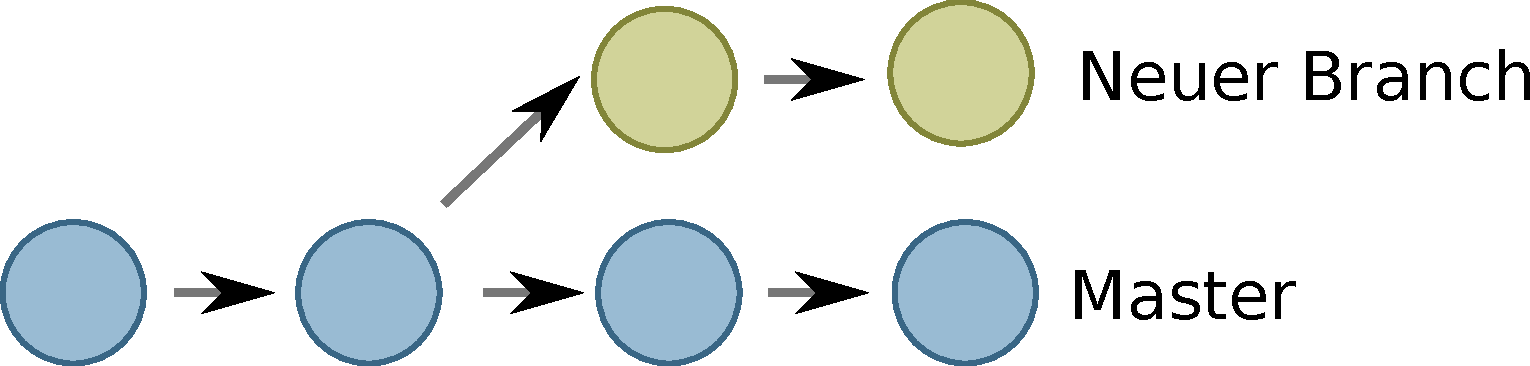
\includegraphics[width=7cm]{bilder/branch.pdf}
\end{center} 
%    \caption{}
%    \label{fig:awesome_image}
\end{figure}

Will man jedoch einen neuen Branch erstellen, um beispielsweise ein neues Feature erst einmal für sich zu programmieren, so benutzt man
\begin{verbatim}
git checkout -b neuer_branch
\end{verbatim}
Wobei \qmarks{neuer\_ branch} der Name des neuen Branches ist, den man erstellen will.

Um zum Master-Branch zurückzuwechseln, verwendet man \qmarks{git checkout master}.

Das Löschen eines Branches funktioniert mit
\begin{verbatim}
git branch -d neuer_branch
\end{verbatim}

Der Branch ist jedoch noch nicht entfernt verfügbar, sondern nur auf der lokalen Maschine.
Um den Branch anderen verfügbar zu machen, muss man ihn erst hochladen:
\begin{verbatim}
git push origin <branch>
\end{verbatim}

Um Änderungen zu aktualisieren, verwendet man hier ebenfalls \qmarks{git pull}.

Will man den aktuellen Branch mit einem anderen zusammenführen, so verwendet man den
\begin{verbatim}
git merge <branch>
\end{verbatim}
Befehl.

Git versucht in beiden Fällen die Änderungen automatisch zusammenzuführen.
Ist dies nicht möglich, so muss man die Änderung selbst durchführen.
Git meldet in diesem Fall Konflikte.
Sind diese Konflikte aufgelöst, so kann man sie wieder mit
\begin{verbatim}
git add <dateiname> 
\end{verbatim}
stagen.

Mit 
\begin{verbatim}
git diff <quell_branch> <ziel_branch>
\end{verbatim}
lassen sich die Unterschiede näher betrachten.

\subsubsection{Zurücksetzen}
\marginpar{Kada}

\begin{figure}[htb]
\begin{center}
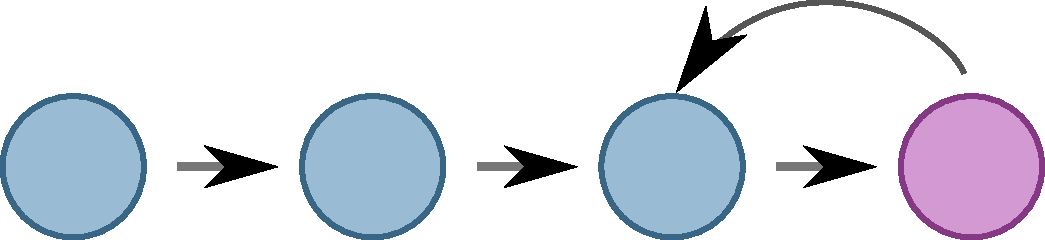
\includegraphics[width=7cm]{bilder/back.pdf}
\end{center} 
%    \caption{}
%    \label{fig:awesome_image}
\end{figure}
Für den den Fall, dass man lokale Änderungen wieder rückgängig machen möchte, kann man mit
\begin{verbatim}
git checkout --<filename>
\end{verbatim}
den Stand auf HEAD zurücksetzen lassen.

Sind die Änderungen bereits im Stage, so muss man sich eine Kopie aus dem entfernten Repository holen.
Die geschieht mit:
\begin{verbatim}
git fetch origin
git reset --hard origin/master
\end{verbatim}

\subsubsection{Forward}
\marginpar{Kada}

\begin{figure}[htb]
\begin{center}
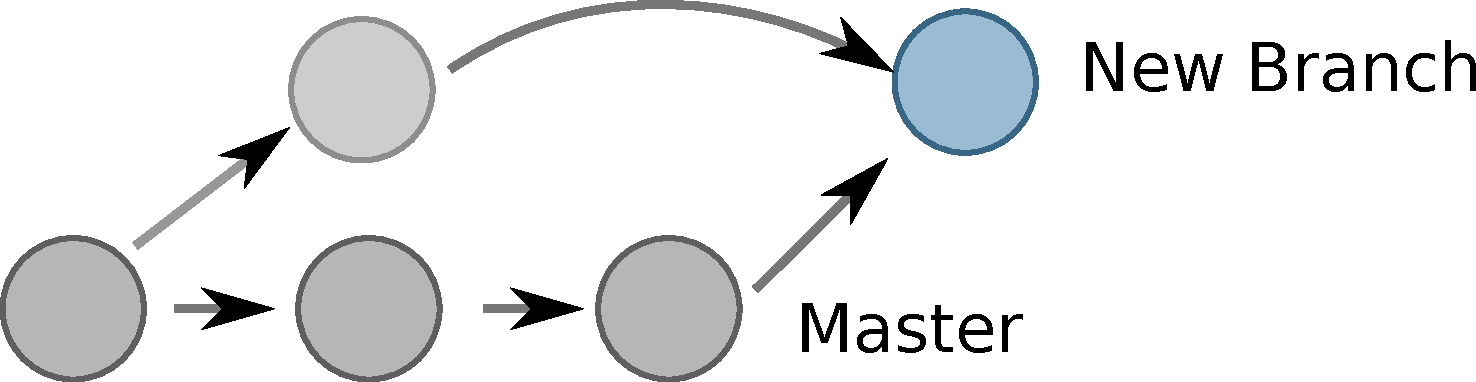
\includegraphics[width=7cm]{bilder/merge.pdf}
\end{center} 
%    \caption{}
%    \label{fig:awesome_image}
\end{figure}
\newpage

\section{Programmiersprache und Hilfsmittel}
\marginpar{Jan}

In diesem Abschnitt werden die programmiertechnischen Hilfsmittel beschrieben und erläutert.
Vor Beginn des einjährigen Projektes stand die Wahl der Programmiersprache zur Debatte.
Zur Auswahl standen C++ und Python, welche beide Vor- und Nachteile besaßen.
Größter Vorteil von Python ist die Kompaktheit, mit der Projekte konstruiert werden können.
Bei C++ stehen jedoch leistungsstarke Bibliotheken zur Verfügung, die neben Vorkenntnissen der Teilnehmer letztendlich den Ausschlag gaben.
% Anmerkung Marcel: War der eigentliche Grund nicht eher die Kenntnisse über die Sprachen? Python fast nicht bekannt und C++ mindestens bei der Hälfte der PG öfter benutzt. (evtl. waren da auch noch Einwände wegen Geschwindigkeit und C++-Python-Bindings?)

Zunächst wird kurz auf die Programmiersprache C++ und die benutze Entwicklungsumgebung, den Qt-Creator, eingegangen.
Zum Ende dieses Abschnittes wird die Bibliothek \textit{SeqAn} vorgestellt, welche zahlreiche Funktionen für die Behandlung von Datenstrukturen aus dem Bereich der Bioinformatik zur Verfügung stellt.
\subsection{C++}
\marginpar{Jan}
Die Programmiersprache C++ wurde von Bjarne Stroustrup entwickelt und erschien 1985 in der ersten Version.
Wie der Name schon andeutet, ist C++ eine Erweiterung der Programmiersprache C um verschiedene Aspekte, wie beispielsweise Klassen \citep{Stroustrup1996}.
Außerdem besteht eine Abwärtskompatibilität zu C, wodurch sich C-Code direkt ausführen lässt.
Nachteilig wirkt sich dadurch aber aus, dass sich viele Designnachteile auch in C++ wiederfinden.
Dazu gehört beispielsweise die Trennung in Headerdateien, welche vom sogenannten Präprozessor geladen werden, und dem eigentlichen Code.
Gemeinsames Designziel beider Sprachen ist aber die Effizienz, welche zum großen Teil durch die Speicherverwaltung erreicht wird.
Es wird kein \textit{Garbage-Collector} eingesetzt, wodurch der Programmierer mehr Kontrolle (aber auch Verantwortung) über das Programm erhält.

Dies steht im Gegensatz zu Java, wo der Aspekt der Plattformunabhängigkeit stärker wiegt als die Effizienz.
Die Unabhängigkeit ist bei C++ nicht (direkt) gegeben, da der Compiler für jedes System den systemspezifischen Maschinencode erzeugt.
Durch den Einsatz des Qt-Creators, der im nächsten Abschnitt beschreiben wird, haben wir eine einfache Möglichkeit, um die Unabhängigkeit über Umwege zu erreichen.

\subsection{Qt-Creator}
\marginpar{Jan}
Als Entwicklungsumgebung setzt unsere Projektgruppe den Qt-Creator ein.
Dieser wurde ursprünglich vom Qt-Projekt für die Entwicklung von plattformunabhängigen grafischen Oberflächen mit der Qt-Bibliothek entwickelt.
Es lassen sich jedoch auch allgemeine C++-Projekte damit entwickeln.

Die Plattformunabhängigkeit ist ein entscheidender Faktor, da alle drei großen Betriebssysteme, Windows, Mac OS und Linux, von den Teilnehmern des Projekts eingesetzt werden.
Wir ersparen uns durch die Nutzung außerdem Portierungsarbeiten, da die Qt-Bibliothek die Programmierung von Multithreading und grafischen Oberflächen vereinfacht.
Auch die Festlegung auf ein Zielsystem entfällt.

\subsection{SeqAn}
\marginpar{Benjamin}

SeqAn ist eine C++-Bibliothek zur Verarbeitung von biologischen Daten. Sie geht
auf ein Forschungsprojekt an der FU Berlin zurück und
stellt effiziente Algorithmen und Datenstrukturen zur Verfügung, die auf
Sequenzen arbeiten. Die Bibliothek ist in C++ implementiert und auf Effizienz
und Erweiterbarkeit optimiert, was durch die rigorose Verwendung von
Template-Metaprogrammierung erreicht wird. Dies stellt auch gleichzeitig den
größten Nachteil von SeqAn dar, da einiges an Einarbeitung erforderlich ist, um
mit dieser Programmierweise umgehen zu können.

Für die Projektgruppe hat sich SeqAn aus mehreren Gründen gegen andere
Bibliotheken durchgesetzt.

\begin{itemize}
	\item Unterstützung aller gängigen und von der Projektgruppe benötigten
          Dateiformate.
    \item Geschwindigkeit und Speicherverbrauch haben eine hohe Priorität.
	\item Sehr große Auswahl an Algorithmen mit dem sehr schnell
          Readmapper-Prototypen entwickelt werden können.
	\item Funktioniert auf vielen verschiedenen Plattformen, insbesondere
          auch unter Windows, was das Testen erleichtert.
\end{itemize}

Unser Readmapper benutzt SeqAn derzeit zur Ein- und Ausgabe von FASTA-,
FASTQ- und VCF-Dateien, zur Auswertung von Kommandozeilenoptionen und zur generellen
Behandlung von DNA-Strings. Hierbei haben sich die verschiedenen unterstützten
Alphabete wie DNA, DNA mit 'N' und IUPAC (siehe Abschnitt~\ref{sec:data:iupac}) als nützlich erwiesen.
Unsere Mapping- und Alignierverfahren nutzen derzeit die in der Bibliothek bereitgestellten Algorithmen nicht als Grundlage, da sie zu stark von den verbreiteten Verfahren, die in SeqAn implementiert sind, abweichen.

\chapter{Biologische Grundlagen}
\label{sec:bio}
\marginpar{Jens}
In diesem Kapitel sollen die für unsere Projektgruppe relevanten biologischen Grundlagen erläutert werden. Die Informationen wurden (wenn nicht anders angegeben) dem Buch \textit{Molekulare Genetik} von Rolf \citet{Knippers2006} entnommen. Dieses Kapitel behandelt dabei die folgenden Themen:
Zunächst werden wir uns (in Abschnitt \ref{sec:bio:dna}) den Aufbau der DNA (dem Träger der Erbinformation) ansehen. Anschließend wird erklärt, was Chromosomen sind (Abschnitt \ref{sec:bio:chromo}) und wie sich Pro- und Eukaryoten unterscheiden (Abschnitt \ref{sec:bio:proeukaryoten}). In Abschnitt \ref{sec:bio:zell} geht es darum, wie die DNA bei der Zellteilung verdoppelt und auf die beiden Tochterzellen aufgeteilt wird. Wir kommen anschließend (in Abschnitt \ref{sec:bio:pbsyn}) zur Protein-Biosynthese, also dem Vorgang, bei dem die auf der DNA gespeicherte Information in Proteine übersetzt wird. Abschnitt \ref{sec:bio:erb} behandelt die Vererbung und soll einige Grundbegriffe der Vererbungslehre erklären. Für unsere Projektgruppe sind vor allem Mutationen des Genoms bzw. der DNA interessant. Welche Arten von Mutationen es gibt, wird in Abschnitt \ref{sec:bio:muta} näher erläutert. Das Ende dieses Kapitels befasst sich mit den verschiedenen Methoden die Basen-Sequenz eines gegebenen DNA-Stücks zu bestimmen.  

\section{DNA}
\label{sec:bio:dna}
\marginpar{Jens}
Die Desoxyribonukleinsäure, kurz DNA\footnote{Die deutsche Abkürzung DNS wird nur noch sehr selten verwendet und ist laut Duden veraltet.} (engl. desoxyribonucleic acid), kommt in allen Lebewesen vor (d.h. zum Beispiel auch  Bakterien) und ist der Träger der Erbinformation. Die DNA enthält somit die Informationen, die die Nachkommen von ihren  Eltern geerbt haben und die für den Bau von Proteinen benötigt werden. Proteine können die verschiedensten Aufgaben  in unserem Körper übernehmen. In Abschnitt \ref{sec:bio:pbsyn:proteine} werden wir genaueres über Proteine erfahren.

DNA-Moleküle bestehen aus einen Doppelstrang von \emph{Nukleotiden}, die miteinander verbunden sind. Diese Nukleotide setzen sich wiederum aus  drei Bausteinen zusammen: Einem Zucker-Molekül (der Desoxyribose), das mit einem Phosphatrest sowie einer von vier möglichen Nukleobasen chemisch verbunden ist. Die Nukleotide können zu einem Strang zusammengesetzt werden, indem das Zuckermolekül des einen Nukleotids mit dem Phosphatrest des nächsten verbunden wird. Die  Zucker-Phosphat-Ketten eines DNA-Moleküls befinden sich im äußeren Bereich des Doppelstrangs und bilden somit das Rückgrat der DNA. Zwischen den beiden Zucker-Phosphat-Ketten sind jeweils zwei Nukleobasen über Wasserstoffbrückenbindungen miteinander verbunden\footnote{Streng genommen besteht ein DNA-Doppelstrang somit aus zwei Molekülen, da nur zwischen Zucker und Phosphatrest sowie zwischen Zucker und Nukleobase chemische Bindungen vorliegen, nicht aber zwischen den Nukleobasen.}.  

\begin{figure}[htbp]
\begin{center}
\begin{minipage}[h]{0.3\textwidth}
\begin{tabular}{rl}
Desoxyribose & \includegraphicstotab[height=12pt]{bilder/DNA_Schema_Desoxyribose} \\
Phosphatrest & \includegraphicstotab[height=12pt]{bilder/DNA_Schema_Phosphatrest} \\
Adenin (\textbf{A})& \includegraphicstotab[height=12pt]{bilder/DNA_Schema_Adenin} \\
Cytosin (\textbf{C}) & \includegraphicstotab[height=12pt]{bilder/DNA_Schema_Cytosin} \\
Guanin (\textbf{G}) & \includegraphicstotab[height=12pt]{bilder/DNA_Schema_Guanin} \\
Thymin (\textbf{T}) & \includegraphicstotab[height=12pt]{bilder/DNA_Schema_Thymin} \\
\end{tabular}
\end{minipage}
\begin{minipage}[h]{0.3\textwidth}
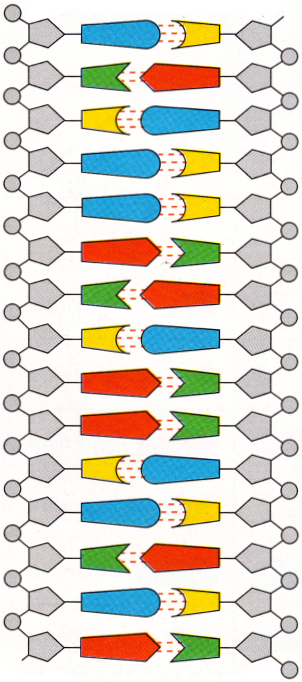
\includegraphics[height=200pt]{bilder/DNA_Schema} %
\end{minipage} %
\end{center} %
\caption{Schematischer Aufbau der DNA. (aus \textit{Lindner Biologie} \citep{Linder}, S. 345/346)}
\label{fig:bio:dna:schema}
\end{figure}

Die Reihenfolge in der diese Nukleobasen (oder einfach kurz Basen) vorkommen, stellen die auf der DNA gespeicherte Information dar. Wie bereits  erwähnt gibt es vier verschiedene Basen, nämlich Adenin, Cytosin, Guanin und Thymin, die jeweils mit ihrem  Anfangsbuchstaben (d.h. A, C, G, T) abgekürzt werden. Eine wichtige Eigenschaft des DNA-Doppelstranges ist die  Komplementarität: Adenin bindet stets an Thymin und Guanin immer an Cytosin. Kennt man also einen Einzelstrang eines DNA-Moleküls, so kann man den fehlenden DNA-Strang rekonstruieren. Adenin und Thymin sind über zwei Wasserstoffbrückenbindungen miteinander verbunden, Cytosin und Guanin mit dreien. Aufgrund ihres chemischen Aufbaus werden Adenin und Guanin als \emph{Purin}-Basen bezeichnet: Sie bestehen aus zwei Kohlenstoff-Stickstoff-Ringen und sind damit ein wenig länger als die \emph{Pyrimidin}-Basen Cytosin und Thymin, die nur aus einem solchen Ring bestehen.

\begin{figure}[htbp]
\begin{center}
\begin{tikzpicture}
	\pgfmathsetmacro{\normDist}{1.15}
	\tikzstyle{bond}=[very thick]
	\tikzstyle{chem}=[black, font=\bfseries\Large]
	\tikzstyle{num}=[blue, font=\bfseries\normalsize]
	
	\node[chem] (C1) at (2*\normDist, 2*\normDist)	{C};
	\node[chem] (H1a) at (2*\normDist, 3*\normDist)	{\color{white}H\color{black}OH};
	\node[chem] (H1b) at (2*\normDist, 1*\normDist)	{H};	
	
	\node[chem] (C2) at (\normDist, 0)	{C};
	\node[chem] (H2a) at (\normDist, -\normDist)	{H};
	\node[chem] (H2b) at (\normDist, \normDist)	{H};	
	
	\node[chem] (C3) at (-\normDist, 0)	{C};
	\node[chem] (H3a) at (-\normDist, -\normDist)	{\color{white}H\color{black}OH};
	\node[chem] (H3b) at (-\normDist, \normDist)	{H};
	
	\node[chem] (C4) at (-2*\normDist, 2*\normDist)	{C};
	\node[chem] (H4) at (-2*\normDist, 1*\normDist)	{H};	
	
	\node[chem] (C5) at (-2*\normDist, 3*\normDist)	{C};
	\node[chem] (H5a) at (-1*\normDist, 3*\normDist)	{H};	
	\node[chem] (H5b) at (-3*\normDist, 3*\normDist)	{H};	
	\node[chem] (H5c) at (-2*\normDist, 4*\normDist)	{\color{white}H\color{black}OH};	
	
	\node[chem] (O) at (0, 2.5*\normDist)	{O};	

	\draw (C1) -- (H1a);
	\draw (C1) -- (H1b);

	\draw (C2) -- (H2a);
	\draw (C2) -- (H2b);
	
	\draw (C3) -- (H3a);
	\draw (C3) -- (H3b);
	
	\draw (C4) -- (H4);
	
	\draw (C5) -- (H5a);
	\draw (C5) -- (H5b);
	\draw (C5) -- (H5c);
	
	\draw[bond] (C1) -- (C2);
	\draw[bond] (C2) -- (C3);
	\draw[bond] (C3) -- (C4);
	\draw[bond] (C4) -- (C5);
	\draw[bond] (C4) -- (O);
	\draw[bond] (O) -- (C1);
	
	\node[num] at (C1.south east) {1'};
	\node[num] at (C2.south east) {2'};
	\node[num] at (C3.south west) {3'};
	\node[num] at (C4.south west) {4'};
	\node[num] at (C5.south west) {5'};
\end{tikzpicture}
\end{center}
\caption{Chemischer Aufbau der Desoxyribose}
\label{fig:bio:dna:desoxyribose}
\end{figure}

Werfen wir einen genaueren Blick auf das Zuckermolekül der DNA: Die \emph{Desoxyribose}, die der DNA ihren Namen gibt, ist ein Zucker-Molekül, das aus fünf Kohlenstoff-Atomen besteht. Diese C-Atome werden wie in Abbildung \ref{fig:bio:dna:desoxyribose} gezeigt von 1‘ bis 5‘ durchnummeriert. Das erste Kohlenstoff-Atom (1‘) ist mit der Nukleobase (A, C, G oder T) verbunden, wobei beim Verbinden Wasser ($\text{H}_2\text{O}$) abgespalten wird. Beim zweiten C-Atom fällt auf, dass hier die Hydroxy-Gruppe fehlt (-H statt -OH); daher kommt die Vorsilbe "`Desoxy"' im Namen des Zuckermolekül. Am 5‘-Ende des Zuckermoleküls hängt die Phosphatgruppe des Nukleotids. Die Phosphatgruppe eines anderen Nukleotids kann mit dem dritten C-Atom des Zucker-Moleküls verbunden werden, sodass sich Ketten aus Phosphatresten und Zucker-Molekülen bilden. 
%#Formulierung
Hier zeigt sich eine weitere wichtige Eigenschaft der DNA: Die beiden Stränge besitzen jeweils eine Richtung. Man kann die Reihenfolge der Nukleobasen in 3‘-5‘-Richtung lesen oder in 5‘-3‘-Richtung. Analysiert man die Struktur der DNA genauer, stellt man fest, dass die beiden DNA-Stränge eines DNA-Moleküls antiparallel zueinander stehen. Ein Strang liegt in 3‘-5‘-Richtung, der andere in 5‘-3‘-Richtung. 

DNA-Moleküle liegen (wie in Abbildung \ref{fig:bio:dna:doppelhelix} gezeigt) als rechtsläufige Doppelhelix vor. Dabei besteht jede Windung aus etwa 10 Basenpaaren und ist 3,4 nm lang. Die Doppelhelix ist nicht exakt symmetrisch, sondern besteht aus einer großen und einer kleinen Furche. Der Durchmesser eines DNA-Doppelstrangs beträgt ca. 2 nm.

\begin{figure}[htbp]
\begin{center}
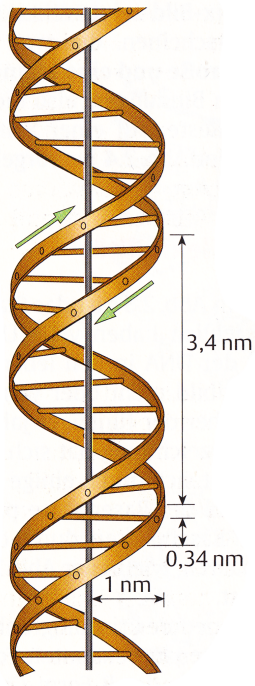
\includegraphics[height=7cm]{bilder/DNA_Helix}
\end{center}
\caption[DNA-Doppelhelix. (aus \citep{Knippers2006}, S. 11)]{DNA-Doppelhelix. Die kleine und große Furche sind deutlich zu erkennen. (aus \citet{Knippers2006}, S. 11)}
\label{fig:bio:dna:doppelhelix}
\end{figure}

\section{Chromosomen}
\label{sec:bio:chromo}
\marginpar{Jens}
DNA-Moleküle können teilweise sehr lang werden, beispielsweise besteht das größte DNA-Molekül des Menschen aus etwa 263 Millionen Basenpaaren. Aus diesem Grund wird die DNA-Doppelhelix um bestimmte Proteine, sogenannte Nukleosomen, herum gewickelt. Durch weitere Proteine wird die DNA weiter zusammengefaltet, wie diese Faltungen jedoch genau aussehen und welche Proteine daran beteiligt sind, ist noch Gegenstand der Forschung \citep{Hansen2012}. 

Der Komplex aus DNA und Proteinen wird als Chromosom bezeichnet. Chromosomen können in drei verschiedenen Formen vorliegen. Kurz vor einer Zellteilung besteht jedes Chromosom aus zwei Chromatinfäden (d.h. zwei DNA-Doppelsträngen), die jeweils dieselbe Information tragen und am \emph{Centromer} miteinander verbunden sind. In schematischen Darstellungen von Chromosomen (wie zum Beispiel Abbildung \ref{fig:bio:chromo:chromosom}) wird fast immer diese Form gezeigt. Während der Zellteilung werden die beiden Chromatinfäden eines Chromosoms auf die beiden Tochterzellen aufgeteilt, sodass das Chromosom nach einer Zellteilung nur noch aus einem Chromatinfaden besteht. Die Chromatinfäden sind während der Zellteilung stark komprimiert und von daher unter einem Lichtmikroskop sichtbar. Zwischen den Zellteilungen liegen die Chromosomen als freies Chromatin vor. Nur in diesem Zustand kann die auf der DNA gespeicherte Information gelesen oder kopiert werden. Unter einem Lichtmikroskop sind die freien, unkomprimierten Chromatinfäden nicht sichtbar.

\begin{figure}[htbp]
\begin{center}
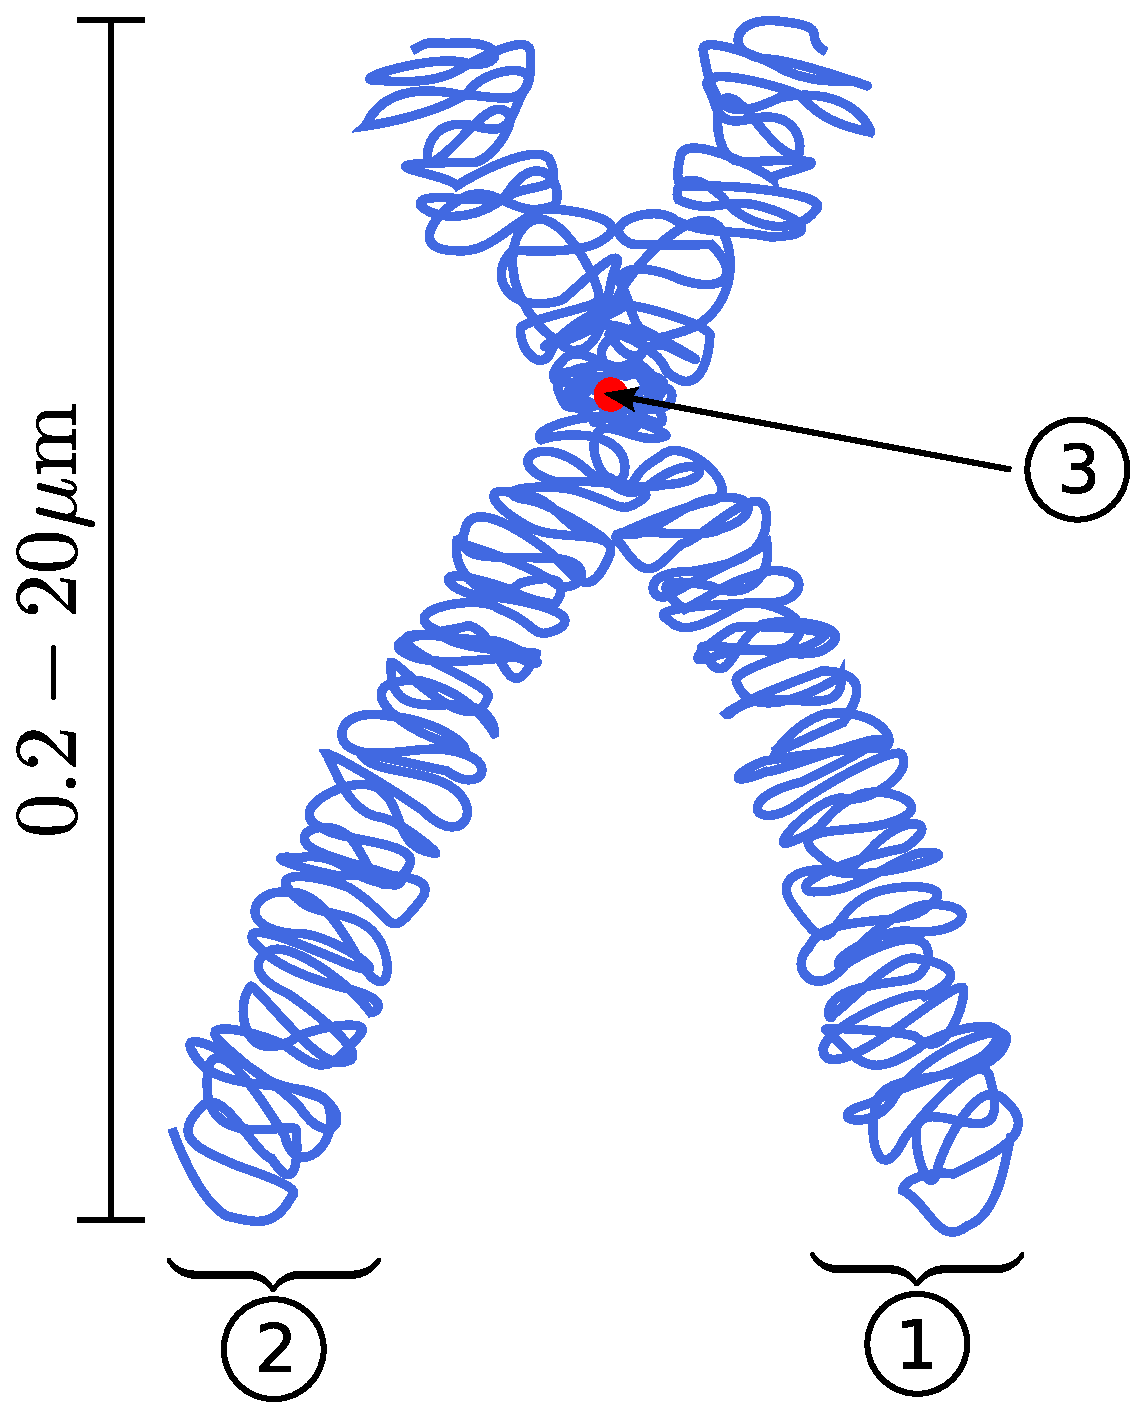
\includegraphics[height=6cm]{bilder/Chromosom}
\end{center}
\caption[Schematische Abbildung eines Chromosoms. (aus \protect\url{http://commons.wikimedia.org/wiki/File:Chromosome.svg})] {Schematische Abbildung eines Chromosoms mit zwei Chromatiden. (1) und (2) die beiden Chromatiden, (3) Centromer. (aus \protect\url{http://commons.wikimedia.org/wiki/File:Chromosome.svg}).}
\label{fig:bio:chromo:chromosom}
\end{figure}

Menschliche Zellen enthalten bis auf wenige Ausnahmen\footnote{Ausnahmen bilden zum einen die Geschlechtszellen, d.h. Spermien bzw. Eizellen (siehe Abschnitt \ref{sec:bio:erb}), sowie Zellen, bei denen sich die Chromosomenzahl durch Krankheiten verändert hat (siehe Abschnitt \ref{sec:bio:muta}).} stets 46 Chromosomen, bzw. 23 Chromosomenpaare. Von jedem Paar haben wir ein Chromosom vom Vater geerbt und eines von der Mutter. Die Informationen, die auf den Chromosomen eines Paares stehen, sind ähnlich, aber nicht zwingend gleich. Das 23. Chromosomenpaar bestimmt das Geschlecht eines Menschen: Frauen haben zwei X-Chromosomen, Männer ein X- und ein Y-Chromosom. Dementsprechend werden diese beiden Chromosomen auch als Geschlechtschromosomen oder kurz Gonosomen bezeichnet. Insgesamt besteht das menschliche Genom (also die Vereinigung aller Chromosomen einer Zelle) aus drei Milliarden Basenpaaren oder kürzer aufgeschrieben 3 Gbp. Die Vorsilbe \emph{G} steht dabei für Giga also $10^9$; \emph{bp} ist die Abkürzung für Basenpaar. Dementsprechend gibt es auch die Einheiten \emph{Mbp} und \emph{kbp} für Millionen bzw. Tausend Basenpaare. Da es für jedes Basenpaar vier Möglichkeiten (A, C, G und T) gibt, beträgt der Informationsgehalt des menschlichen Genoms sechs Milliarden Bit bzw. 750 MB. An dieser Stelle soll nochmal erwähnt werden, dass jede Zelle eines Lebewesens denselben DNA-Code enthält, d.h. jede menschliche Zelle enthält die erwähnten drei Milliarden Basenpaare. 

\begin{figure}[htbp]
\begin{center}
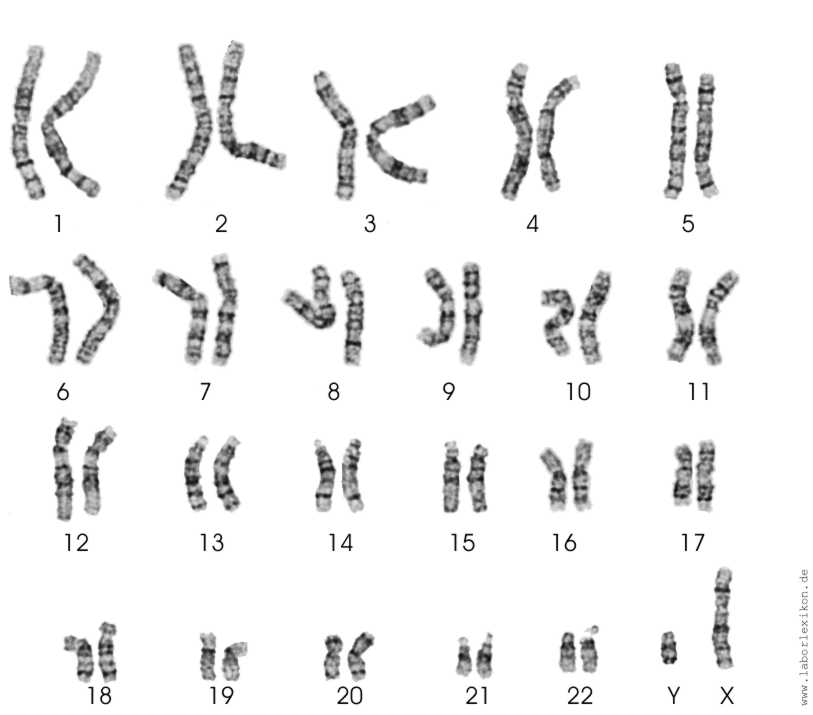
\includegraphics[width=0.8\textwidth]{bilder/Karyogramm}
\end{center}
\caption{Karyogramm des Menschen. (aus \protect\url{http://www.laborlexikon.de/images/Karyogramm-813.JPG})}
\label{fig:bio:chromo:karyogramm}
\end{figure}

\section{Prokaryoten und Eukaryoten}
\label{sec:bio:proeukaryoten}
\marginpar{Jens}

An einigen Stellen ist es wichtig zwischen Pro- und Eukaryoten zu unterscheiden. Eukaryoten sind alle höheren Lebensformen, das heißt Menschen, Tiere, Pflanzen und Pilze. Zu Prokaryoten gehören Bakterien und die Archaebakterien, die auch als Urbakterien bezeichnet werden. Eukaryotische Zellen besitzen die im vorherigen Abschnitt erwähnten Chromosomen, die sich im Zellkern befinden. Prokaryotische Zellen besitzen dagegen keinen Zellkern, ihre DNA ist somit nicht durch eine Membran von den restlichen Zellorganellen abgegrenzt. Des Weiteren enthalten Prokaryoten in der Regel nur ein DNA-Molekül, das ringförmig, also in sich geschlossen ist. 

Da wir uns vor allem mit dem menschlichen Genom beschäftigen, sind für uns hauptsächlich Eukaryoten von Interesse. Trotzdem wird an einigen Stellen erklärt, welche Unterschiede zu Prokaryoten bestehen.

\paragraph{Aufbau einer eukaryotischen Zelle}

Jede Zelle ist von einer Zellmembran umgeben, die die Zelle von der Umgebung abgrenzt. Im Innern der Zellen befinden sich verschiedene, sogenannte Organellen, die bestimmte Funktionen in der Zelle übernehmen. Zu diesen gehört unter anderen der Zellkern, in dem sich die DNA befindet. Das endoplasmatische Retikulum ist mit seinen Ribosomen an der Protein-Biosynthese beteiligt, also an der Übersetzung eines DNA-Abschnitts in ein Protein. In Abschnitt \ref{sec:bio:pbsyn} werden wir mehr dazu erfahren. Der Raum, der zwischen der Zellmembran und den einzelnen Organellen liegt, wird als Zytoplasma bezeichnet. Zellen enthalten noch weitere Organellen, eine Beschreibung dieser würde hier aber zu weit führen. Die Mitochondrien sollen trotzdem kurz erwähnt werden:

\begin{figure}[htbp]
\begin{center}
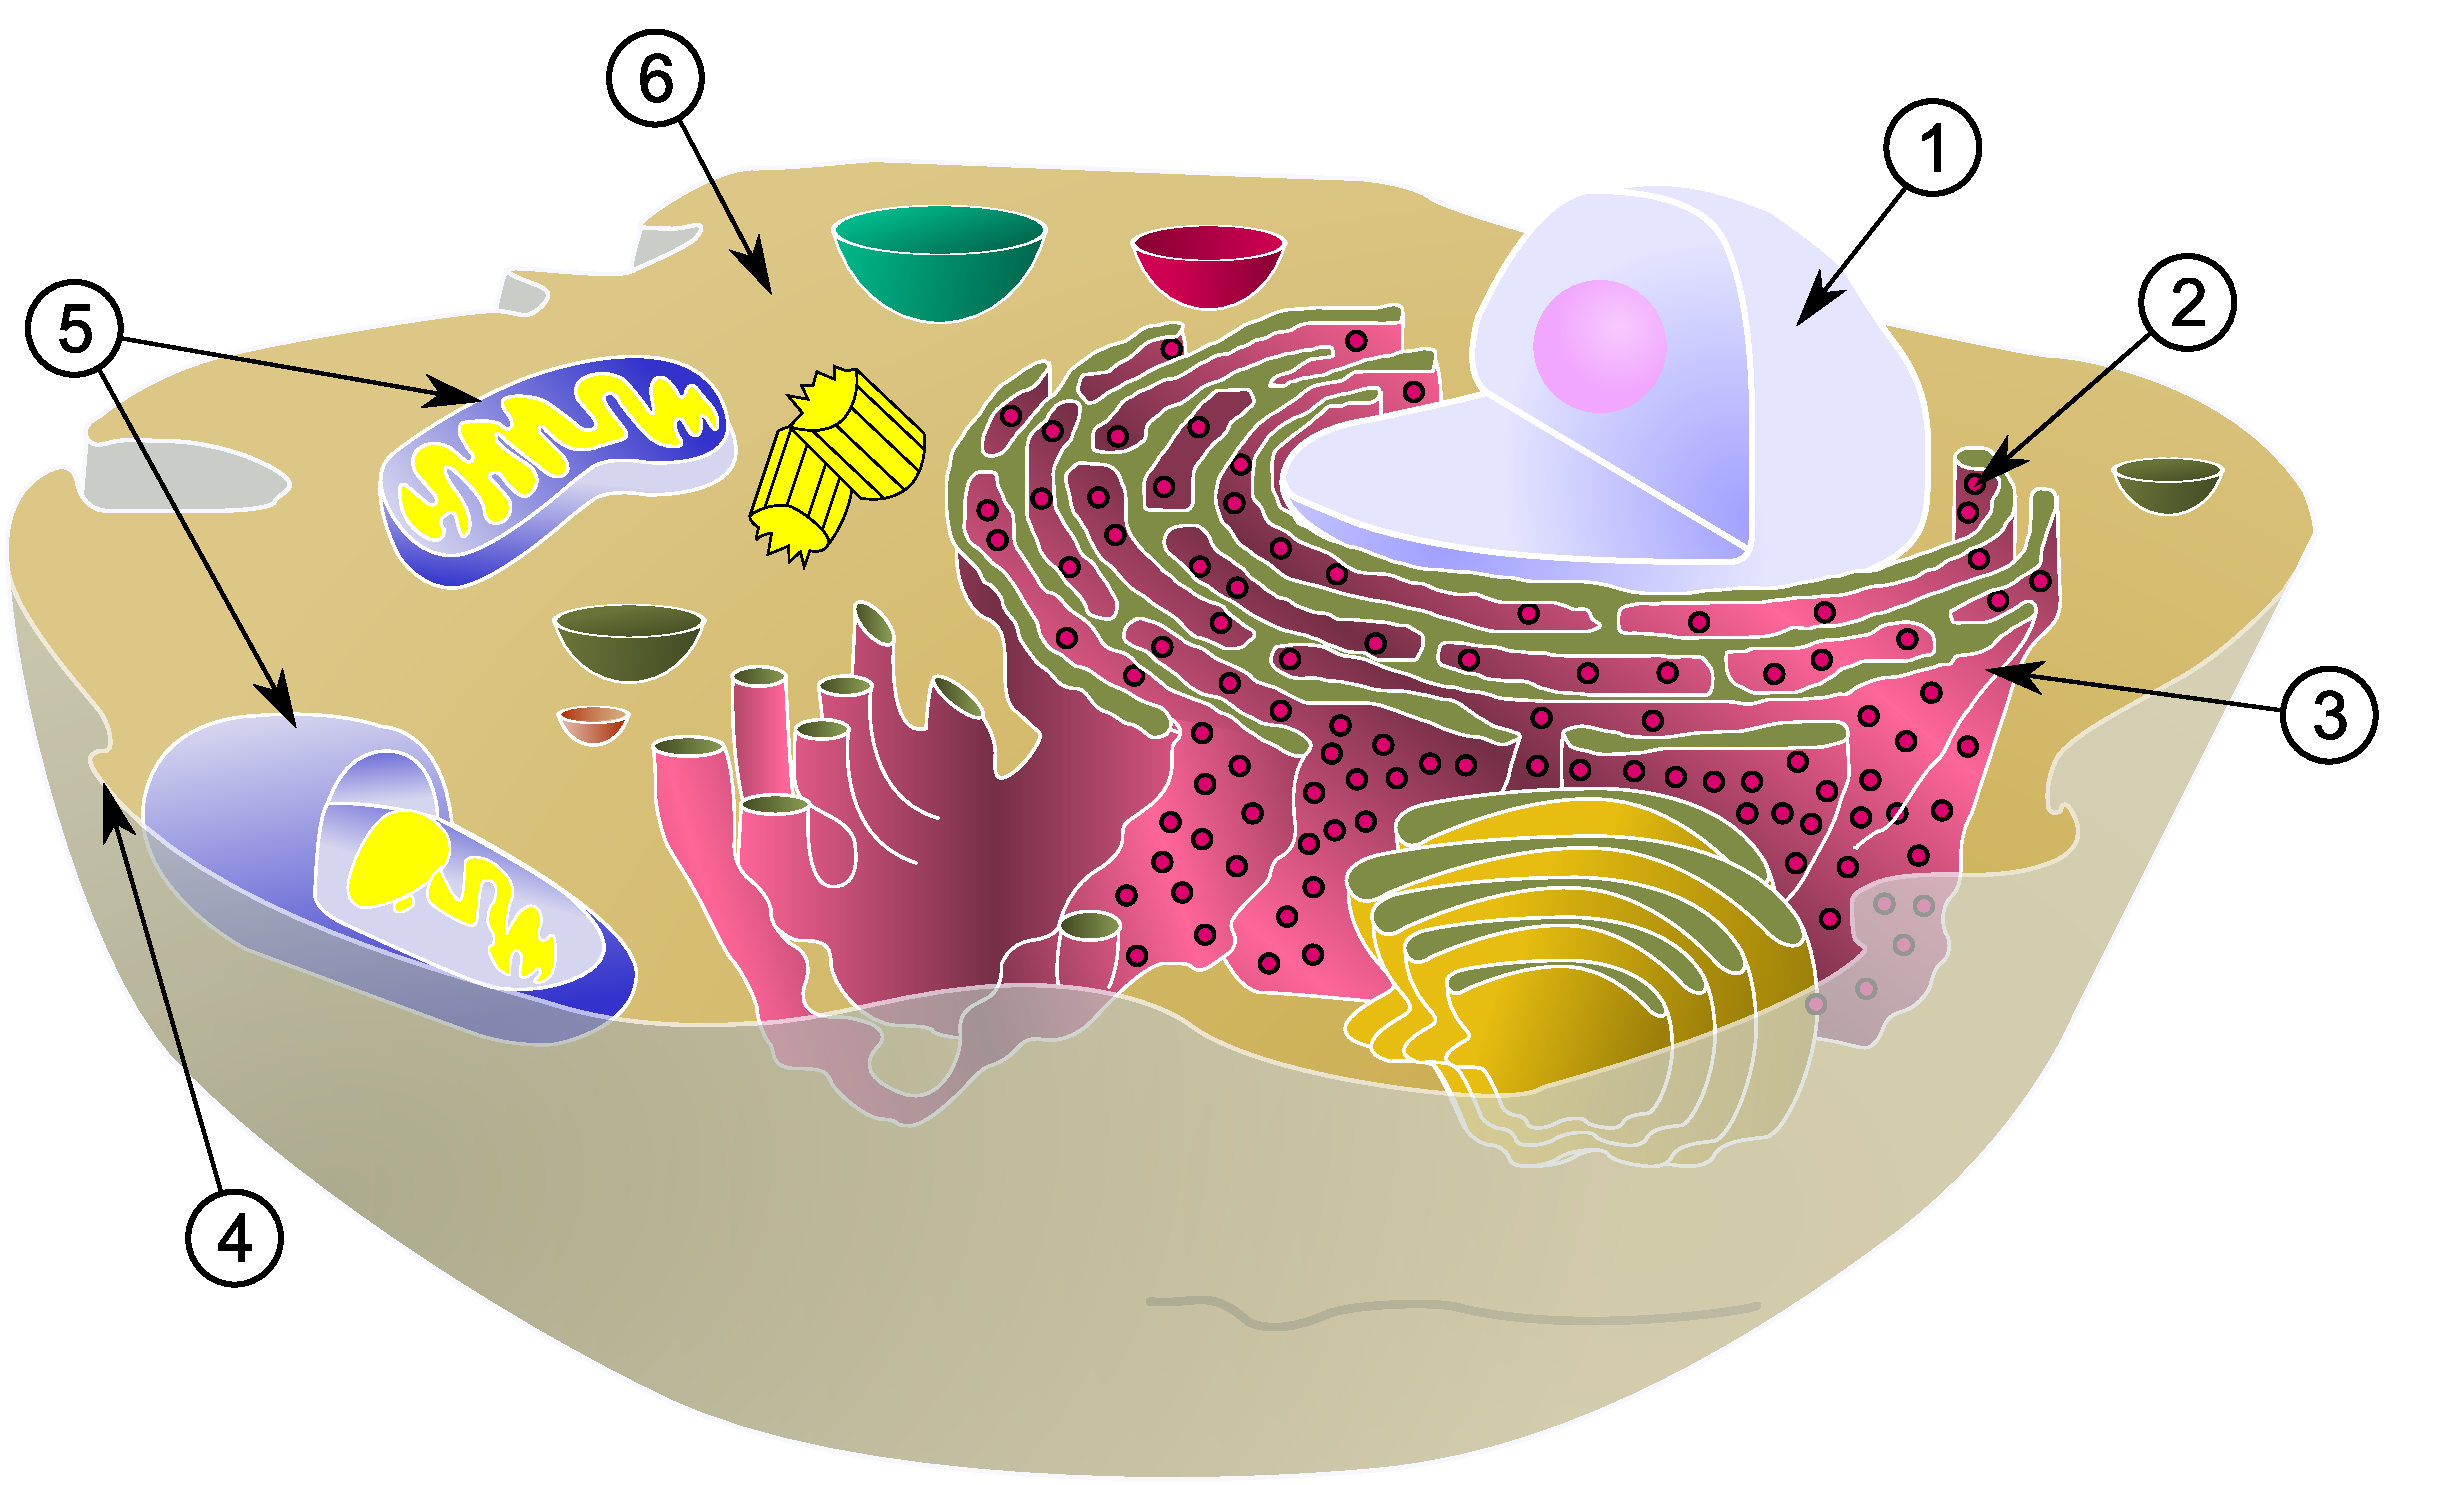
\includegraphics[width=0.95\textwidth]{bilder/Zelle}
\end{center}
\caption[Typische eukaryotische Tierzelle. (aus \protect\url{http://commons.wikimedia.org/wiki/File:Biological_cell.svg})] {Typische eukaryotische Tierzelle. (1) Zellkern, (2) Ribosom, (3) Endoplasmatisches Retikulum, (4) Zellmembran, (5) Mitochondrien, (6) Zytoplasma. (aus \protect\url{http://commons.wikimedia.org/wiki/File:Biological_cell.svg})}
\label{fig:bio:zelle}
\end{figure}

\paragraph{Mitochondrien}

Mitochondrien sind im Prinzip die \textit{Energiekraftwerke} unserer Zellen. Sie stellen Adenosintriphosphat (kurz ATP) her, dass bei sehr vielen Prozessen in unserem Körper als Energieträger genutzt. Wird eine Phosphatgruppe von ATP abgespalten, entsteht Adenosindiphosphat (kurz ADP) und Energie wird frei. Die freiwerdende Energie wird beispielsweise in Muskelzellen als mechanische Arbeit umgesetzt. Auch die für die Herstellung organischer Moleküle benötigte Energie wird durch ATP bereitgestellt. In den Mitochondrien werden ADP und der Phosphatrest wieder zu ATP verbunden. Die dafür nötige Energie liefert zum Beispiel Glucose (Traubenzucker), das direkt oder auch indirekt über die Nahrung aufgenommen wird.

Das in diesem Bericht die Mitochondrien erwähnt werden, hat aber einen anderen Grund: Bisher wurde immer behauptet, dass sich die gesamte DNA einer Zelle im Zellkern befindet. Das ist nicht ganz richtig: Mitochondrien enthalten ebenfalls einen eigenen, kurzen DNA-Ring. Beim Menschen hat dieser DNA-Ring eine Länge von 16.569 Basenpaaren \citep{Mitomap} und enthält zahlreiche überlebenswichtige Gene.

\section{Zellteilung}
\label{sec:bio:zell}
\marginpar{Jens}

Wie bereits erwähnt, enthalten alle Zellen dieselbe DNA-Information. Teilt sich eine Zelle, so muss ihre DNA zunächst verdoppelt werden. Dieser Vorgang wird DNA-Replikation genannt. Anschließend wird bei der Mitose die replizierte DNA auf beide Tochterzellen gleichmäßig aufgeteilt, sodass sich die Zelle teilen kann. Wir schauen uns zunächst die DNA-Replikation an:

\subsection{DNA-Replikation}
\label{sec:bio:zell:repli}
\marginpar{Jens}

Bei der DNA-Replikation, also der Verdopplung der DNA sind eine ganze Reihe an Proteinen beteiligt. Zunächst entwindet die \emph{Topoisomerase} die DNA-Doppelhelix, sodass sie durch die \emph{Helicase} in die zwei Einzelstränge gespalten werden kann. Die eigentliche Replikation wird nun von der \emph{DNA-Polymerase} durchgeführt. Diese liest den DNA-Strang in 3'-5'-Richtung. Dementsprechend wird der neu gebildete DNA-Strang stets am 3'-Ende verlängert.
%
Als Ausgangsmaterial verwendet die DNA-Polymerase \emph{Desoxyribonukleosidtriphosphate} (dNTPs). Diese bestehen aus einem Zuckermolekül (der Desoxyribose), einer der vier Nukleobasen (also Adenin, Cytosin, Guanin oder Thymin) sowie einer Triphosphat-Gruppe. Je nach dem welche Base in dem Molekül verbaut ist, wird dNTP auch als dATP, dCTP, dGTP bzw. dTTP bezeichnet. Bei der DNA-Synthese werden die (zum Original-Strang komplementären) dNTPs unter Abspaltung von Diphosphat miteinander verbunden, sodass sich wieder ein DNA-Doppelstrang mit komplementären Basenpaaren bildet.

Aufgrund der Antiparallelität der DNA (die beiden Stränge eines DNA-Moleküls laufen in entgegengesetzte Richtungen) findet nur beim 3'-5'-Strang eine kontinuierliche Synthese statt. Die Helicase spaltet den DNA-Doppelstrang immer weiter auf, sodass die die DNA-Polymerase beliebig lange weiterarbeiten kann. Der Strang, bei dem die Synthese kontinuierlich stattfindet, wird als Leitstrang bezeichnet. Im Gegensatz dazu findet beim Folgestrang, der in 5'-3'-Richtung verläuft, eine diskontinuierliche Synthese statt. Die DNA-Polymerase arbeitet hier ebenfalls in 3'-5'-Richtung und entfernt sich somit immer weiter von der Helicase. Irgendwann trifft die DNA-Polymerase auf ein bereits repliziertes DNA-Stück, sodass sich die DNA-Polymerase von der DNA löst. Der Bereich zwischen Helicase und bereits verdoppelter DNA wird nun von einer weiteren DNA-Polymerase repliziert, wobei sich diese wiederum von der Helicase entfernt. Es entstehen sogenannte \emph{Okazaki-Fragmente}. Diese werden durch ein weiteres Protein, der \emph{Ligase}, miteinander verbunden, sodass wieder ein ununterbrochener DNA-Doppelstrang vorliegt. 

\begin{figure}[htbp]
\begin{center}
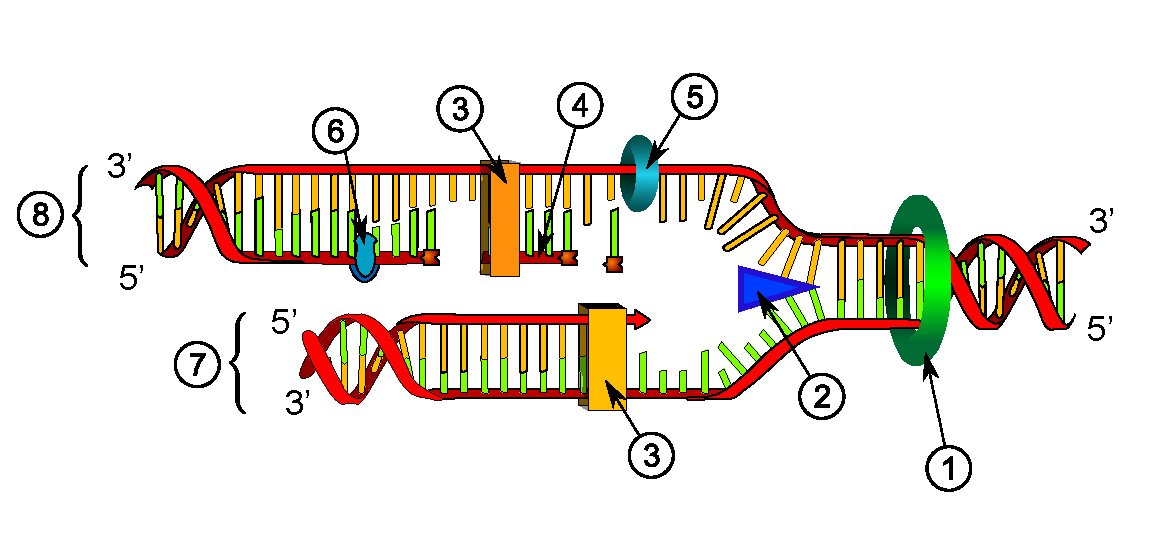
\includegraphics[width=\textwidth]{bilder/DNA_Replikation}
\end{center}
\caption[DNA-Replikation. (aus \protect\url{http://de.wikipedia.org/wiki/Datei:DNA_replication_de.svg})] {DNA-Replikation. (1) Topoisomerase, (2) Helicase, (3) Polymerase, (4) Okazaki-Fragment, (5) Primase, (6) Ligase, (7) Leitstrang (kontinuierliche Synthese), (8) Folgestrang. (aus \protect\url{http://de.wikipedia.org/wiki/Datei:DNA_replication_de.svg})}
\label{fig:bio:zell:repli}
\end{figure}

Aufgrund der Komplementarität der DNA sind die beiden hergestellten Doppelstränge exakte Kopien voneinander. Die neu synthetisierte DNA in 5'-3'-Richtung am Leitstrang entspricht dem originalen 5'-3'-Strang des Folgestranges. Analog dazu gleichen sich auch der alte und neue Strang in 3'-5'-Richtung.

Nach der DNA-Replikation bestehen die Chromosomen aus zwei Chromatiden, die am Centromer miteinander verbunden sind. Die DNA-Doppelstränge in den beiden Chromatiden sind exakte Kopien voneinander. Da die Chromosomen eines Chromosomenpaares ähnliche Informationen enthalten, kann es also sein, dass direkt nach der DNA-Replikation bestimmte Code-Sequenzen in der Zelle in vierfacher Ausführung vorkommen.

\subsection{Mitose}
\label{sec:bio:zell:mitose}
\marginpar{Jens}

Nach der DNA-Replikation findet die eigentliche Zellteilung statt. Hierbei muss die DNA gleichmäßig auf beide Tochterzellen aufgeteilt werden. Dieser Vorgang wird Kernteilung oder in Fachsprache Mitose genannt und besteht aus mehreren Phasen.

In der \emph{Prophase} kondensieren die Chromosomen, sodass sie unter einem Lichtmikroskop sichtbar werden. Sie haben jetzt die kompakte, charakteristische Form mit zwei Chromatiden. Während der \emph{Prometaphase} löst sich die Kernhülle auf. Außerdem wird von den gegenüberliegenden Seiten der Zelle ein Spindelapparat ausgebaut. Die Spindeln heften sich in der \emph{Metaphase} an die Centromere der Chromosomen. In der \emph{Anaphase} werden die beiden Chromatiden der Chromosomen durch den Spindelapparat auseinander gezogen, sodass sich auf beiden Seiten der Zelle 46 Chromosomen mit jeweils einem Chromatid befinden. In der \emph{Telophase} bilden sich dann zwei neue Kernhüllen -- auf jeder Seite der Zelle eine. Gleichzeitig dekondensieren die Chromosomen, d.h. sie breiten sich wieder aus und werden damit unter dem Lichtmikroskop unsichtbar. Die Teilung des Zellkerns ist damit abgeschlossen. 

\begin{figure}[htb]
\begin{center}
\begin{tikzpicture}
	\pgfmathsetmacro{\dst}{3}
	\tikzstyle{textnode}=[font=\bfseries\large];
	\tikzstyle{arr}=[-latex, very thick, shorten >=1ex, shorten <=1ex, bend angle=10, bend left];
	\node (inter) at (-2*\dst, 0)
		{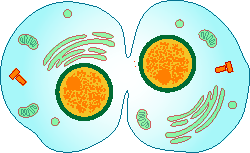
\includegraphics[height=2.8cm]{bilder/Mitose_Interphase}};
	\node (pro) at (-\dst, 1.5*\dst)
		{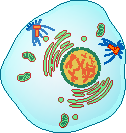
\includegraphics[height=2.8cm]{bilder/Mitose_Prophase}};
	\node (prometa) at (\dst, 1.5*\dst)
		{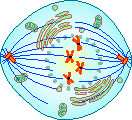
\includegraphics[height=2.8cm]{bilder/Mitose_Prometaphase}};
	\node (meta) at (2*\dst, 0)
		{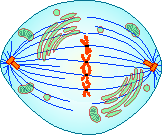
\includegraphics[height=2.8cm]{bilder/Mitose_Metaphase}};
	\node (ana) at (\dst, -1.5*\dst)
		{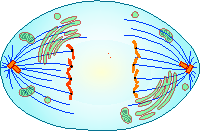
\includegraphics[height=2.8cm]{bilder/Mitose_Anaphase}};
	\node (telo) at (-\dst, -1.5*\dst)
		{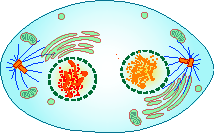
\includegraphics[height=2.8cm]{bilder/Mitose_Telophase}};
		
	\draw[arr] (inter) to (pro);
	\draw[arr] (pro) to (prometa);
	\draw[arr] (prometa) to (meta);
	\draw[arr] (meta) to (ana);
	\draw[arr] (ana) to (telo);
	\draw[arr] (telo) to (inter);
	
	\node[textnode, below=0cm of ana] {Anaphase};
	\node[textnode, below=0cm of telo] {Telophase};
	\node[textnode, above=0.2cm of inter, left] {Interphase};
	\node[textnode, above=0.2cm of meta, right] {Metaphase};
	\node[textnode, above=0cm of prometa] {Prometaphase};
	\node[textnode, above=0cm of pro] {Prophase};
\end{tikzpicture}
\end{center}
\caption{Mitose. (aus \protect\url{http://de.wikipedia.org/wiki/Mitose})}
\label{fig:bio:zell:mitose}
\end{figure}

In der \emph{Interphase}, die in der Regel nicht mehr zur Mitose gezählt wird, teilt sich die Zelle, sodass jede Tochterzelle genau einen Zellkern mit dem vollen Chromosomensatz enthält. Während der Interphase findet auch die Proteinbiosynthese (siehe Abschnitt \ref{sec:bio:pbsyn}) statt, bei der die auf der DNA speicherten Informationen genutzt werden, um Proteine herzustellen. Die Interphase ist also quasi der \textit{normale} Zustand einer Zelle. Vor einer erneuten Zellteilung wird die DNA repliziert. Auch dieser Vorgang gehört zur Interphase.

\subsection{Künstliche DNA-Replikation - PCR}
\label{sec:bio:zell:pcr}
\marginpar{Jens}

Die DNA-Replikation, die vor jeder Zellteilung stattfindet, kann auch künstlich im Reagenzglas durchgeführt werden. Mit Hilfe der Polymerase-Ketten-Reaktion (PCR, engl. Polymerase Chain Reaction) können bereits geringste DNA-Mengen vervielfältigt werden. Zum Erstellen eines genetischen Fingerabdrucks (zum Beispiel bei Mordfällen) werden hinreichend große DNA-Mengen benötigt. Findet man am Tatort beispielsweise eine Hautzelle des Täters, kann die darin enthaltende DNA mit Hilfe der PCR vervielfacht werden. Ohne dieses Verfahren wäre es nicht ohne weiteres möglich, von einer so geringen DNA-Menge einen genetischen Fingerabdruck zu erstellen. Weitere Anwendungen sind Vaterschaftstests oder der Nachweis von Erbkrankheiten. Auch für die Sequenzierung (siehe Abschnitt \ref{sec:bio:seq}), also das Bestimmen der Nukleotid-Abfolge eines DNA-Moleküls, werden hinreichend große DNA-Mengen benötigt. Die PCR ist somit die Grundlage für zahlreiche Anwendungsfälle, bei denen man DNA in hinreichend großer Menge benötigt. 

Die PCR funktioniert dabei folgendermaßen: Zunächst wird die DNA auf 94$^\circ$C erhitzt, wodurch der DNA-Doppelstrang in zwei Einzelstränge gespalten wird (Denaturierung). Bei 70$^\circ$C können sich nun Primer an die DNA lagern. Primer sind kurze DNA-Sequenzen und werden von der DNA-Polymerase als Startpunkte benötigt. Die Wahl der guter Primer ist wichtig, aber auch sehr schwierig: Optimal wäre es, wenn sich die Primer nur an die 3'-Enden der DNA heften, sodass die Polymerase die gesamte DNA vervielfältigen kann. Würden sich die Primer an die Mitte oder gar an das 5'-Ende der DNA lagern, wird ein großer Teil der DNA nicht vermehrt, da die DNA-Polymerase nur in 3'-5'-Richtung arbeitet. Zudem sollte sich nur ein Primer an die jeden DNA-Strang lagern, da sonst bei der Replikation nicht miteinander verbundene Fragmente entstehen.

Nachdem sich die Primer an die DNA gelagert haben, replizieren DNA-Polymerasen die DNA-Stränge. Aus dem ursprünglichen DNA-Doppelstrang entstehen so zwei Kopien. Der beschriebene Zyklus kann beliebig häufig wiederholt werden, wobei natürlich hinreichend viele freie Nukleotide als Ausgangsstoff für die Polymerase vorhanden sein müssen.

Das Erhitzen und Abkühlen übernehmen spezielle Geräte (sogenannte Thermocycler). Sie wiederholen den beschrieben Zyklus der PCR beliebig oft. Da sich bei jeden Schritt die DNA-Menge verdoppelt, steigt die Anzahl der DNA-Kopien exponentiell an: Bereits nach 20 Zyklen liegen theoretisch eine Millionen Kopien vor.

Ein Problem existiert allerdings noch: Bei 94$^\circ$ wird nicht nur die DNA denaturiert, sondern es zersetzen sich auch gewöhnliche DNA-Polymerasen irreversibel. Früher (als die PCR-Methode 1986 eingeführt wurde) wurden tatsächlich nach jeden Zyklus neue Polymerasen zugesetzt. Eine entscheidende Verbesserung lieferte die Taq-Polymerase des Bakteriums \emph{Thermus aquaticus}. Das Bakterium gehört zu den thermophilen, also zu den wärmeliebenden Bakterien und lebt beispielsweise in heißen Quellen oder Geysiren. Seine DNA-Polymerase ist auch noch bei Temperaturen über 94$^\circ$ stabil.

\section{Protein-Biosynthese}
\label{sec:bio:pbsyn}
\marginpar{Jens}


Unter Protein-Biosynthese versteht man die Übersetzung eines DNA-Abschnitts (eines sogenannten Gens) in ein Protein. Dieser Vorgang unterteilt sich in zwei Abschnitte:

Zunächst wird bei der \emph{Transkription} ein Gen der DNA abgelesen und eine RNA-Kopie erstellt. Die Ribonukleinsäure, kurz RNA, ist ähnlich wie DNA aufgebaut, es gibt jedoch drei Unterschiede: Im Gegensatz zur DNA besteht RNA nur aus einem Einzelstrang. Des Weiteren enthält sie als Zuckermolekül -- wie ihr Name bereits vermuten lässt -- die Ribose anstatt der Desoxyribose. Statt der Base Thymin wird in der RNA Uracil verbaut. Chemisch gesehen unterscheidet sich Uracil durch eine fehlende Methyl-Gruppe von Thymin, die möglichen Basenpaarungen sind aber dieselben, d.h. Uracil verbindet sich stets mit Adenin und umgekehrt. Die transkribierte RNA wird auch als messanger-RNA oder kurz mRNA bezeichnet.

Im zweiten Schritt der Proteinbiosynthese wird die mRNA in eine Aminosäure-Sequenz übersetzt. Dieser Vorgang wird als \emph{Translation} bezeichnet. Aminosäure-Sequenzen sind die Vorstufen von Proteinen. 


\subsection{Transkription}
\label{sec:bio:pbsyn:transkription}
\marginpar{Jens}


Bei der Transkription erstellt ein bestimmter Protein-Komplex, die sogenannte  RNA-Polymerase, eine mRNA-Kopie eines DNA-Abschnitts. Dieser Vorgang kann in drei Phasen unterteilt werden:

Bei der \emph{Initiation} setzt sich eine RNA-Polymerase an den Promotor eines Gens. Der Promotor ist eine spezielle DNA-Sequenz, die Informationen darüber enthält, wann und in welchen Zelltyp ein Gen transkribiert soll. Der Promotor codiert somit selbst kein Protein, sondern reguliert die Genexpression. Diese Regulation ist sehr wichtig, da jede Zelle dieselbe DNA-Information enthält. Eine Magenzelle muss beispielsweise ganz andere Proteine herstellen als eine Nervenzelle im Gehirn.

In der zweiten Phase, der \emph{Elongation}, wird die DNA von der RNA-Polymerase in 3'-5'-Richtung abgelesen und eine komplementäre mRNA-Kopie erstellt. Die Synthese der RNA erfolgt somit in 5'-3'-Richtung. 

Nachdem das Gen abgelesen wurde, löst sich die RNA-Polymerase vom DNA-Strang. Dieser Vorgang wird das \emph{Termination} bezeichnet, es ist allerdings noch ungeklärt, wann die Termination genau stattfindet bzw. wodurch sie eingeleitet wird. 


\subsection{Proteine}
\label{sec:bio:pbsyn:proteine}
\marginpar{Jens}
Bevor wir uns der Translation widmen, bei der die mRNA in ein Protein übersetzt wird, wollen wir zunächst klären, was überhaupt Proteine sind: Proteine bestehen aus Aminosäuren, von denen 20 verschiedene in der Natur vorkommen (siehe Abbildung \ref{fig:bio:pbsyn:amino}). Aminosäuren können miteinander verbunden werden und bilden dann Aminosäure-Sequenzen, die auch als Polypeptide bezeichnet werden. Proteine können aus mehren solcher Polypeptide bestehen, wobei die Faltung der Aminosäuren-Sequenzen für die Funktion entscheidend ist.

\begin{figure}[htbp]
\begin{center}
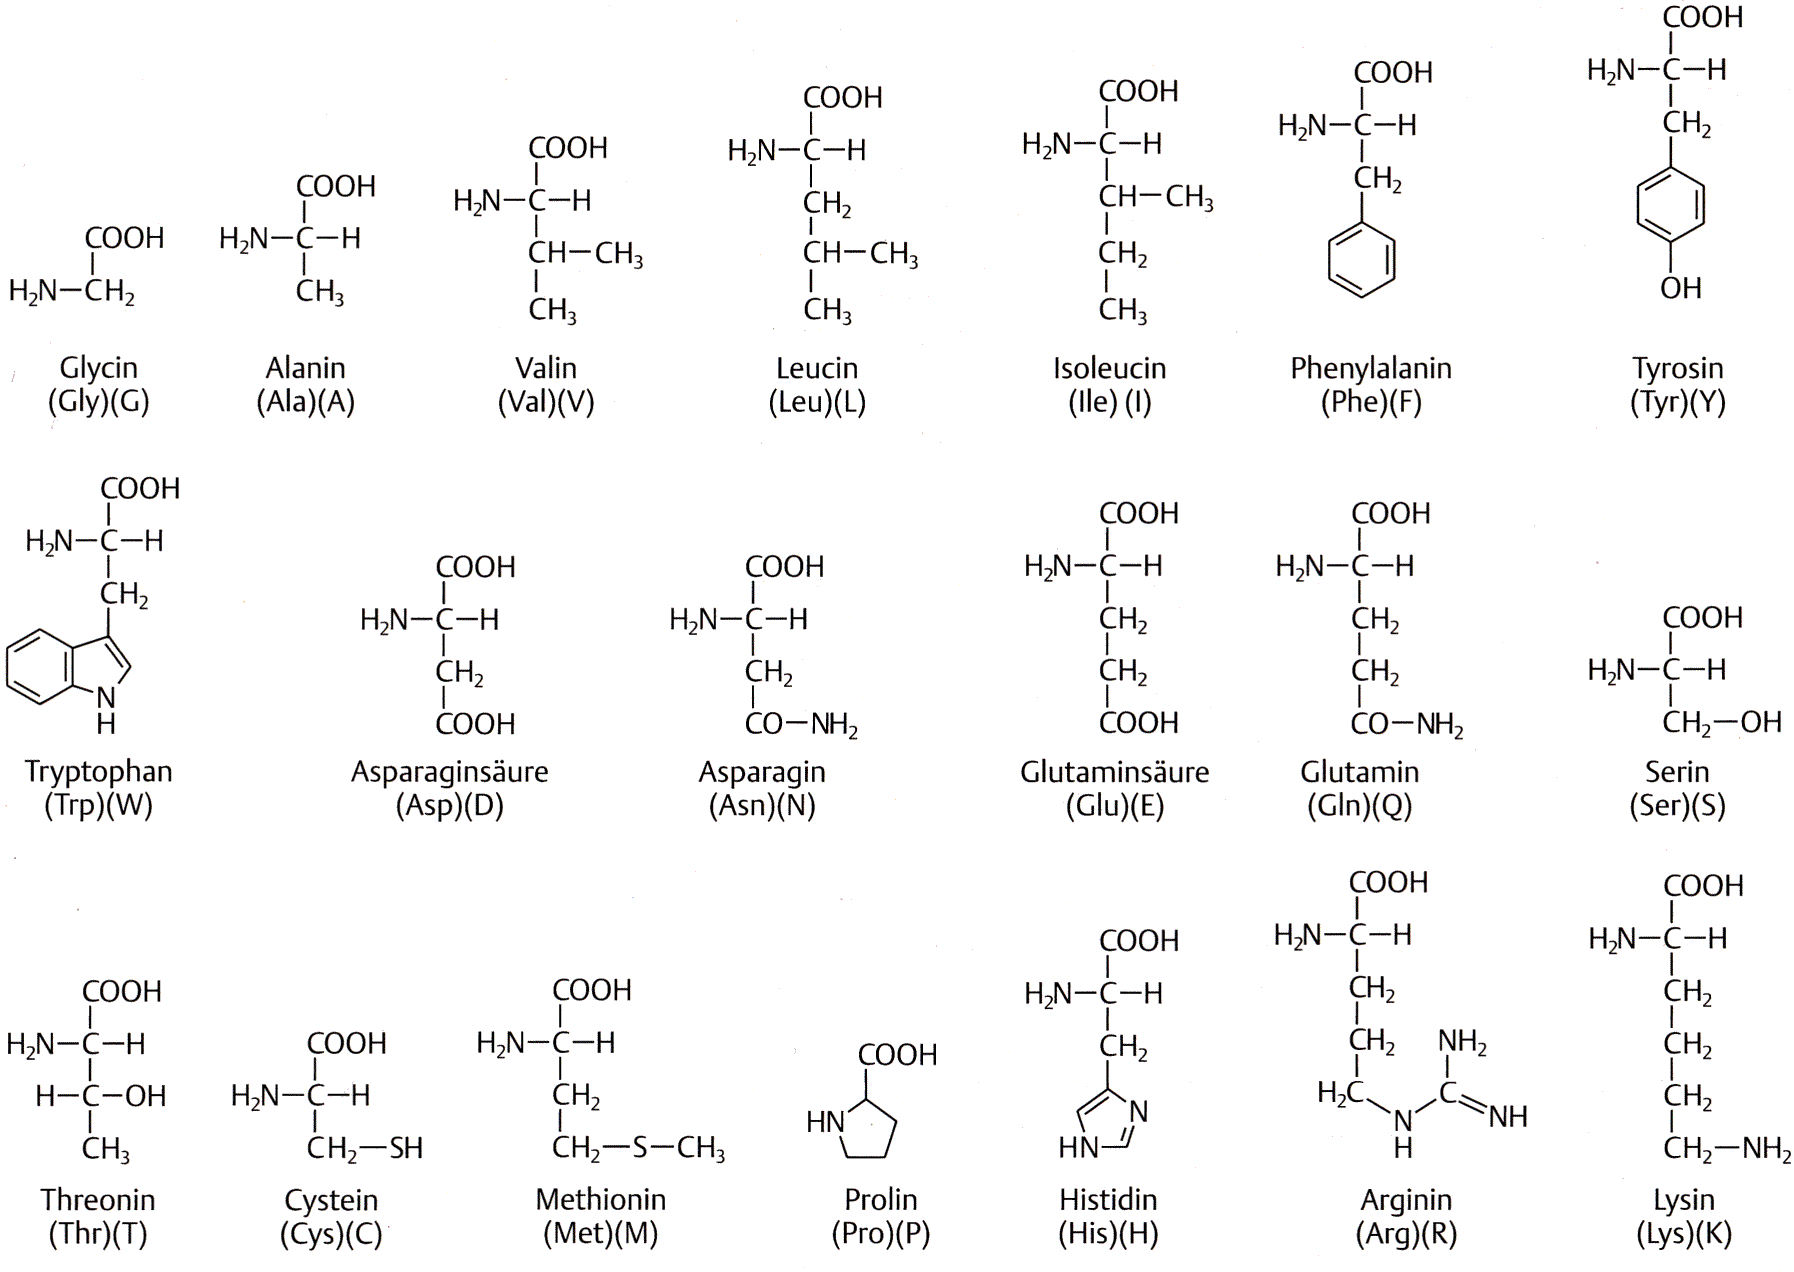
\includegraphics[width=0.8\textwidth]{bilder/Aminoacids}
\end{center}
\caption{Übersicht der 20 natürlich vorkommenden Aminosäuren. (aus \citet{Knippers2006}, S. 38)}
\label{fig:bio:pbsyn:amino}
\end{figure}

Proteine können die unterschiedlichsten Aufgaben im Organismus übernehmen: Das Protein Hämoglobin sorgt beispielsweise in unserem Blut dafür, dass Sauerstoff von den Lungenbläschen zu den Zellen transportiert wird. Proteine, die als Katalysator für chemische Reaktionen dienen, werden auch Enzyme genannt. Als Beispiel könnte man Lactase nennen, ein Enzym, dass Milchzucker (Lactose) in Galactose und Glucose (Traubenzucker) spaltet. Es gibt noch viele weitere Funktionen, die Proteine erfüllen können, beispielsweise als Ionen-Kanal in der Zellmembran.

Die Aminosäuren aus denen Proteine bestehen werden häufig mit drei Buchstaben abgekürzt (z.B. Gly für Glycin, Ala für Alanin, usw.). Darüber hinaus gibt es einen Ein-Buchstaben-Code, die verwendeten Buchstaben überschneiden sich aber mit den Abkürzungen für die Nukleobasen in DNA und RNA. So wird beispielsweise die Aminosäure Glycin ebenso mit G abgekürzt wie auch die Base Guanin.




\subsection{Translation}
\label{sec:bio:pbsyn:translation}
\marginpar{Jens}

Unter Translation versteht man die Übersetzung der mRNA in ein Protein. Die Translation der Eukaryoten unterscheidet sich von der Translation der Prokaryoten. Bei Prokaryoten (d.h. Bakterien und Archaebakterien) findet die Translation noch während der Transkription statt. Bei Eukaryoten ist die Translation räumlich von der Transkription getrennt. Außerdem findet bei Eukaryoten eine Nachverarbeitung der mRNA statt. Dieser Vorgang wird Prozessierung genannt und in Abschnitt \ref{sec:bio:pbsyn:prozess} genauer erklärt. Nach der Prozessierung verlässt die reife mRNA durch eine Kernpore den Zellkern. Die eigentliche Translation läuft dann ähnlich wie bei Prokaryoten ab und soll nun genauer erklärt werden.

Wie bereits erwähnt, codiert ein mRNA-Strang eine Aminosäure-Sequenz. Es gibt jedoch 20 verschiedene Aminosäuren, aber nur vier verschiedene Basen (A, C, G und U) in der mRNA. Aus diesem Grund bilden immer drei Basen ein sogenanntes Codon und codieren eine Aminosäure. In der Code-Sonne (siehe Abbildung \ref{fig:bio:pbsyn:codesonne}) können wir ablesen, welche Basentripletts welche Aminosäure codieren.


\begin{figure}[htb]
\begin{center}
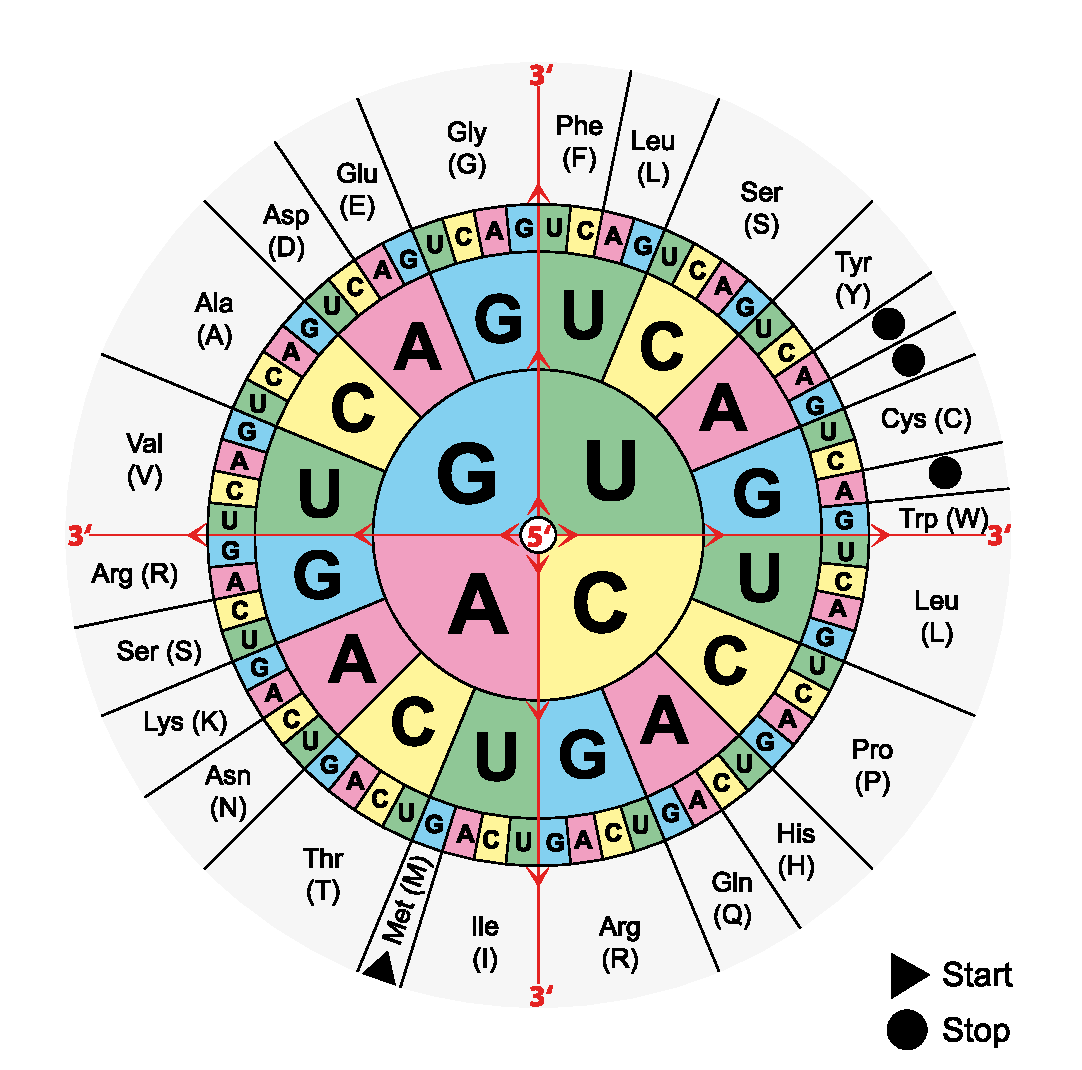
\includegraphics[width=0.7\textwidth]{bilder/Genetischer_Code}
\end{center}
\caption[Genetischer Code. (aus \protect\url{http://commons.wikimedia.org/wiki/File:Aminoacids_table.svg})]{Genetischer Code. Die Basentripletts der mRNA in 5'-3'-Richtung werden (von innen nach außen gelesen) in die gezeigten Aminosäuren übersetzt. (aus \protect\url{http://commons.wikimedia.org/wiki/File:Aminoacids_table.svg})}

\label{fig:bio:pbsyn:codesonne}
\end{figure}

Die Translation findet in 5'-3'-Richtung statt, dementsprechend wird die Code-Sonne von innen nach außen gelesen. Die in der Code-Sonne gezeigte Übersetzung von Codons in Aminosäuren wird auch als genetischer Code bezeichnet.

Die Translation übernehmen die Ribosomen einer Zelle. Sie verbinden sich mit dem mRNA-Strang und lesen ihn solange, bis sie auf das Startcodon AUG treffen. Erst jetzt wird mit der eigentlichen Translation begonnen. Transfer-RNA-Moleküle (kurz tRNA) transportieren je eine Aminosäuren zum Ribosomen. Dazu besitzt die tRNA ein zum entsprechenden Codon komplementäres Anticodon, wobei für jede Aminosäure mindestens eine tRNA existiert. tRNA ist eine besondere Form der RNA: Sie besitzt teilweise Doppelstrangstrukturen und Schleifen, sowie spezielle modifizierte Basen. Im Ribosom verbindet sich das Codon der mRNA mit dem Anticodon einer passenden tRNA. Das Ribosom fügt die von der tRNA transportierte Aminosäure an die aktuelle Aminosäure-Sequenz an. Dieser Vorgang wird so lange durchgeführt, bis das Ribosom auf eines der drei möglichen Stopp-Codons trifft (UAA, UAG und UGA). Hier endet die Translation und das fertige Polypeptid löst sich vom Ribosom. Typischerweise bestehen Proteine aus 100 bis 800 Aminosäuren, es gibt aber auch weitaus größere Proteine.  

\subsection{Prozessierung}
\label{sec:bio:pbsyn:prozess}
\marginpar{Jens}

Bei Eukaryoten findet zwischen Transkription und Translation eine Nachverarbeitung der mRNA statt. Bei diesem Vorgang, den man auch als Prozessierung bezeichnet, wird die sogenannte \emph{prä-mRNA} in \emph{reife mRNA} umgewandelt. Dabei passiert folgendes:

%Bei Eukaryoten findet im Zellkern eine Nachverarbeitung der gerade transkribierten mRNA statt. Vor dieser Nachverarbeitung wird die mRNA auch \emph{prä-mRNA} genannt und nach dieser \emph{reife mRNA}. Bei dieser Nachverarbeitung, die auch Prozessierung genannt wird, passiert folgendes:

Im Gegensatz zu Prokaryoten (bei denen die Translation noch während der Transkription stattfindet) muss die mRNA bei Eukaryoten zwischen Transkription und Translation einen weiten Weg zurücklegen. Zellen enthalten Enzyme, die versuchen jegliche mRNA abzubauen. Um die prä-mRNA davor zu schützen wird ein zusätzliches, modifiziertes Guanin-Nukleotid am 5'-Ende angebracht. Dieser Vorgang wird als \emph{Capping} bezeichnet. Auch die \emph{Polyadenylierung}, bei der das 3'-Ende der mRNA mit Adenin-Nukleotiden verlängert wird, dient der Verhinderung des vorzeitigen Abbaus. Für uns sind aber vor allem das Splicing und RNA-Editing interessant, bei der die codierenden Bereiche der prä-mRNA nachträglich verändert werden.

\paragraph{RNA-Editing}
Beim RNA-Editing werden einzelne Basen der mRNA verändert, sodass zum Beispiel andere Aminosäuren im Protein verbaut werden. Dadurch unterscheidet sich die reife mRNA von der komplementären DNA-Vorlage. Als Beispiel für RNA-Editing sei das Apolipoprotein B genannt. Dieses kommt in zwei verschiedenen Formen in unserem Körper vor: In Leberzellen in der langen Form mit 4536 Aminosäuren, in Dünndarmzellen in der kurzen Form mit 2153 Aminosäuren. Beide Formen entstehen aus derselben prä-mRNA und damit aus demselben DNA-Abschnitt. Die Ursache für die zwei verschiedenen Formen ist das erwähnte RNA-Editing. In den Dünndarmzellen wird an einer bestimmten Stelle in der prä-mRNA Cytosin in Uracil umgewandelt. Dadurch entsteht ein Stopp-Codon, sodass eine entsprechend kürzere Aminosäure-Sequenz gebildet wird. 

RNA-Editing kommt bei Eukaryoten sehr häufig vor. Teilweise werden hierbei auch spezielle Basen (wie zum Beispiel Inosin) verbaut. Solche speziellen Basen kommen zum Beispiel an vielen Stellen der tRNA vor.

\paragraph{Splicing}
Unter Splicing versteht man der Herausschneiden bestimmter Bereiche der prä-mRNA. Die prä-mRNA besteht aus Exons und Introns. Die Introns werden beim Spleißen herausgeschnitten. Die übrigen Abschnitte codieren Proteine und werden Exons genannt.

Beim \emph{alternativen Splicing} kann eine prä-mRNA auf verschiedene Weisen gespleißt werden. Beispielsweise kann es vorkommen, dass in manchen Zellen bestimmte Exons übersprungen oder andere Exons eingebaut werden. Eine weitere Möglichkeit sind alternative Spleißstellen. Hierbei wird nur ein Teil eines Exons übersprungen. Abbildung \ref{fig:bio:pbysn:splicing} veranschaulicht die verschiedenen Möglichkeiten des alternativen Splicings. Ein Gen (also ein DNA-Abschnitt) kann somit wie beim RNA-Editing verschiedene Proteine codieren. 

\begin{figure}[htbp]
\begin{center}
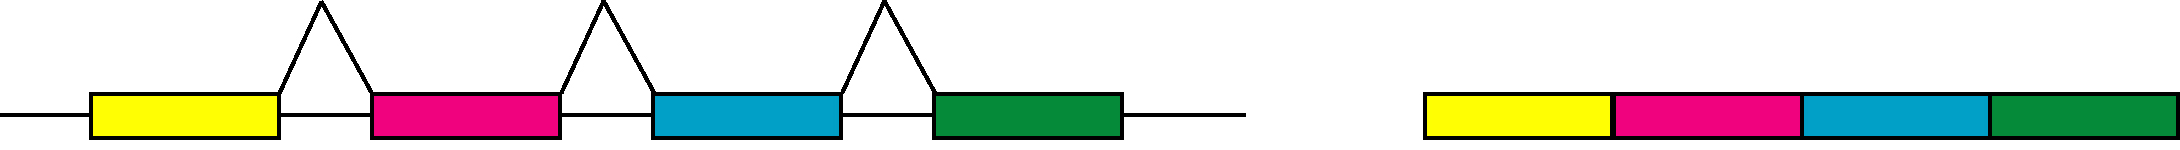
\includegraphics[width=0.7\textwidth]{bilder/Splicing_1} \\
Gewöhnliches Splicing \\
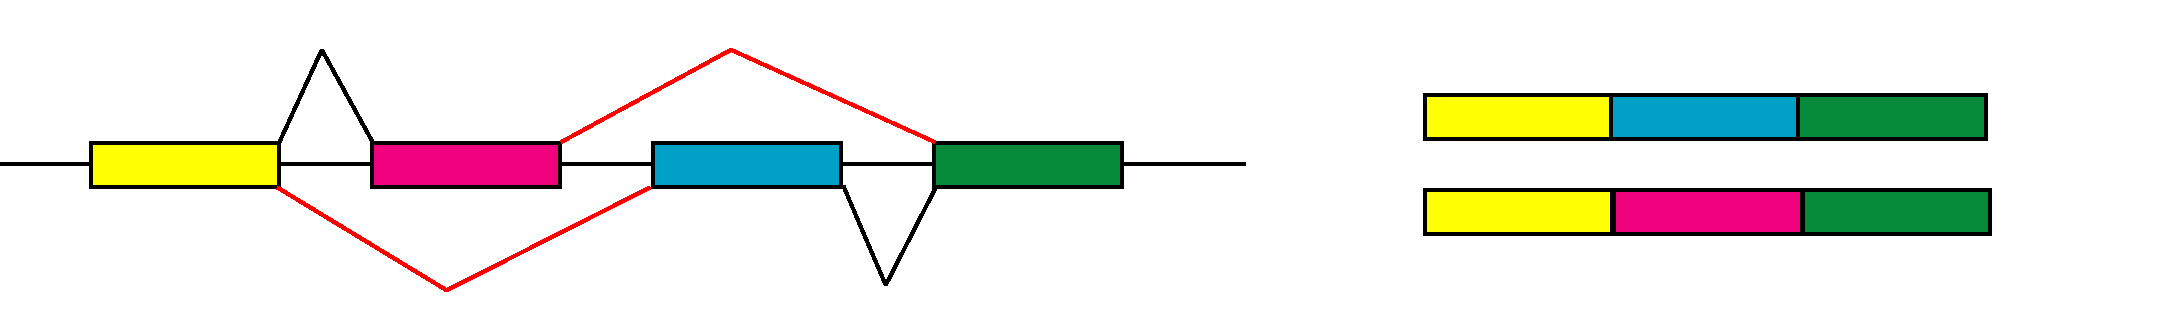
\includegraphics[width=0.7\textwidth]{bilder/Splicing_4} \\
Überspringen von Exons \\
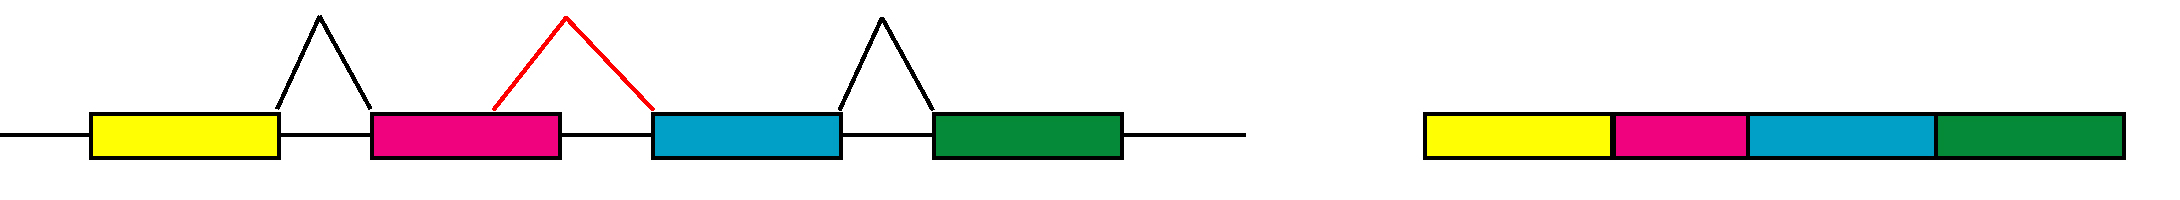
\includegraphics[width=0.7\textwidth]{bilder/Splicing_5} \\
Alternative 5'-Spleißstelle \\
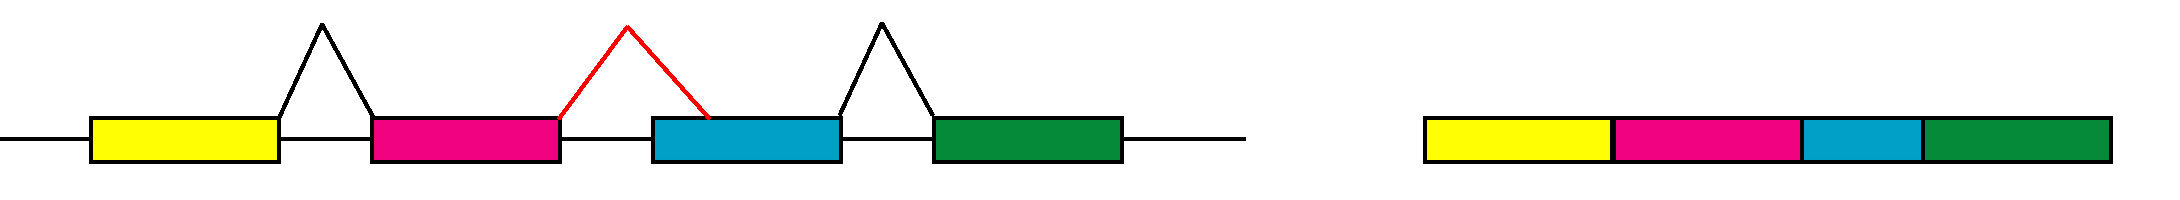
\includegraphics[width=0.7\textwidth]{bilder/Splicing_6} \\
Alternative 3'-Spleißstelle
\end{center}
\caption[Alternatives Splicing (aus \protect\url{http://commons.wikimedia.org/wiki/File:Alternative_splicing.jpg})]{Verschiedene Möglichkeiten beim alternativen Splicing. (aus \protect\url{http://commons.wikimedia.org/wiki/File:Alternative_splicing.jpg})}
\label{fig:bio:pbysn:splicing}
\end{figure}

\section{Vererbung}
\label{sec:bio:erb}
\marginpar{Jens}

Die auf der DNA enthaltene Information wird an die Nachkommen weitervererbt. Dabei ergibt sich jedoch folgendes Problem: Würden Vater und Mutter jeweils ihre 46 Chromosomen weitervererben, so hätte das Kind 92 Chromosomen. Mit jeder weiteren Generation würde sich die Chromosomenzahl erneut verdoppeln. Aus diesem Grund besitzen Eizellen und Spermien nur einen haploiden Chromosomensatz, der aus 23 Chromosomen besteht, und zwar von jedem Chromosomenpaar genau eines. Alle anderen Zellen unseres Körper sind diploid und besitzen somit 46 Chromosomen. Die Halbierung der Chromosomenzahl findet bei der Meiose statt und soll hier nur kurz erläutert werden soll:
\newpage

\subsection{Meiose}
\label{sec:bio:erb:meiose}
\marginpar{Jens}

Zu Beginn der Meiose findet eine Replikation der DNA statt, sodass die Chromosomen der Zelle aus zwei Chromatiden bestehen. Während der ersten Reifeteilung baut sich ähnlich wie bei der Mitose ein Spindelapparat aus. Im Unterschied zur Mitose werden aber nicht die Schwester-Chromatiden voneinander getrennt, sondern die homologen Chromosomen (d.h. die beiden Chromosomen eines Chromosomenpaares). Nachdem sich die Zelle geteilt hat, liegen zwei Zellen mit haploiden Chromosomensatz vor, deren Chromosomen aber immer noch aus zwei Chromatiden bestehen. Bei der zweiten Reifeteilung werden nun analog zur Mitose die Chromatiden voneinander getrennt, sodass letztendlich vier haploide Zellen mit 1-Chromatid-Chromosomen vorliegen.

Während der ersten Reifeteilung kann ein Crossing-Over stattfinden. Dabei werden DNA-Sequenzen zwischen den homologen Chromosomen ausgetauscht. Die Chromosomen eines Kindes sind somit keine exakten Kopien der Chromosomen der Großeltern. Durch das Crossing-Over erhöht sich die genetische Vielfalt, was für das Überleben einer Art sehr vorteilhaft sein kann.

\subsection{Grundbegriffe der Vererbungslehre}
\marginpar{Jens}

Der Begriff Gen wurde bisher schon mehrfach benutzt, allerdings noch nicht genau definiert. Eine eindeutige Definition ist schwierig zu formulieren, fest steht aber, dass es sich bei einem Gen um einen Abschnitt auf DNA handelt. Im Laufe der Geschichte gab es viele Versuche, den Begriff Gen festzulegen. Nach der Entdeckung der DNA-Struktur (1953) wurde ein Gen als ein Abschnitt auf der DNA gesehen, der die Information zur Herstellung eines Proteins trägt. Jedoch insbesondere bei Eukaryoten codiert ein und derselbe DNA-Abschnitt häufig verschiedene Proteine. Wir haben dies bereits beim RNA-Editing und beim alternativen Spleißen kennen gelernt (siehe Abschnitt \ref{sec:bio:pbsyn:prozess}). Darüber hinaus gibt es DNA-Abschnitte, die zur Herstellung der Transfer-RNA oder anderer besonderer RNA dienen (siehe Abschnitt \ref{sec:bio:pbsyn:translation}). Aus diesem Grund, wird heutzutage ein Gen als ein DNA-Abschnitt definiert, der die Information zur Herstellung einer biologisch aktiven RNA enthält. Dabei kann es sich um mRNA handeln, die später in ein Protein übersetzt wird, aber auch um andere RNA-Typen, wie zum Beispiel die erwähnte tRNA. 

Gene können in zwei oder mehr unterschiedlichen Ausbildungsformen vorliegen, die als \emph{Allele} bezeichnet werden. Unter \emph{Genotyp} verstehen wir die Gesamtheit der Gene eines Individuums, unter \emph{Phänotyp} sein äußeres Erscheinungsbild. \emph{Dominante} Allele wirken bei der Ausbildung des Phänotyps bestimmend und unterdrücken \emph{rezessive} Allele in ihrer Wirkung. 

Ein Beispiel soll die gerade genannten Begriffe verdeutlichen. Beim Menschen gibt es vier verschiedene Blutgruppen, die sich anhand der gebildeten Blutgruppensubstanz unterschieden. Bei Blutgruppe A wird die Substanz A gebildet, bei Blutgruppe B die Substanz B, bei AB beide Substanzen, bei 0 keine von beiden. Ursache für die verschiedenen Blutgruppen sind drei Allele eines Gens. Das Allel $i^A$ codiert die Blutgruppensubstanz A, $i^B$ die Substanz B. Beim Allel $i$ wird keine Blutgruppensubstanz gebildet. Die Allele $i^A$ und $i^B$ wirken dominant. Wenn sie vorliegen, wird immer die jeweilige Substanz gebildet. Das rezessive Allel $i$ kommt nur zur Wirkung, wenn kein dominantes Allel vorhanden ist. Da jedes Gen in zweifacher Ausführung vorkommt (nämlich auf den beiden homologen Chromosomen eines Paares), besitzen wir immer zwei Allele. Eines haben wir von der Mutter geerbt, das andere vom Vater. Nun können wir den verschiedenen Phänotypen (also den Blutgruppen) die  möglichen Genotypen zuordnen. Bei Blutgruppe 0 müssen beide Allele vom Typ $i$ sein. Der Genotyp ist also $ii$. Bei Blutgruppe AB werden beide Blutgruppensubstanzen gebildet, als Genotyp kommt also nur $i^Ai^B$ in Frage. Bei Blutgruppe A und B gibt es jeweils zwei Möglichkeiten, nämlich $i^Ai$ und $i^Ai^A$ (bzw. $i^Bi$ und $i^Bi^B$).

Liegen auf den homologen Chromosomen dieselben Allele vor, so nennen wir dies reinerbig oder \emph{homozygot}. Sind die Allele unterschiedlich, so liegt das Gen mischerbig oder \emph{heterozygot} vor.

\section{Mutationen}
\label{sec:bio:muta}
\marginpar{Jens}

Mutationen sind eine dauerhafte Veränderung des Erbgutes. Man unterscheidet drei verschiedene Arten von Mutationen:

Bei einer \textbf{Genom-Mutation} liegt eine Veränderung der Chromosomenzahl vor. Menschen mit einer Genom-Mutationen haben also mehr oder auch weniger als 46 Chromosomen. Eine mögliche Ursache sind Fehler bei der Meiose (oder auch bei Mitose, wenn nur einzelne Zellen des Organismus betroffen sind). Ein bekanntes Beispiel ist die Trisomie 21, besser bekannt als Down-Syndrom. Das 21. Chromosomenpaar liegt hier dreifach vor, was sich bei den Betroffenen unter anderem in einer geistigen Behinderung äußert.

Unter \textbf{Chromosomen-Mutationen} versteht man die strukturelle Veränderung eines Chromosoms. Beispielsweise können durch ungleiches Crossing-Over bei der Meiose Teile von Chromosomen verloren gehen. Als Beispiel könnte man das Katzenschrei-Syndrom nennen, bei dem ein kleiner Teil des 5. Chromosoms fehlt.

Für unsere Projektgruppe sind aber vor allem die \textbf{Gen-Mutationen} relevant:

\subsection{Gen-Mutationen}
\label{sec:bio:muta:gen}
\marginpar{Jan}

Eine Gen-Mutation bezeichnet eine Veränderung einer Basenpaarsequenz innerhalb eines Gens. Unterschieden wird zwischen Punktmutationen, an denen sich ein einzelnes Nukleotid verändert (Substitution), und Rasterverschiebungen, welche durch sogenannte \textbf{Indels} ausgelöst werden. Dieses Wort vereint die Veränderungen von Basenpaaren durch Einfügen (\textbf{In}sertion) oder Entfernen (\textbf{Del}etion) \citep{Knippers2006}. Schwerwiegend werden diese Änderungen, wenn durch die veränderte Sequenz andere Proteine kodiert werden. Bei der bereits genannten \textbf{Leseraster-Mutation} entsteht durch Einfügen oder Löschen von 1 oder 2 Basenpaaren\footnote{Da eine Aminosäure durch jeweils drei Nukleotide kodiert wird, kommt es auch bei Einfügen und Löschen von 4 und 5 (7 oder 8 usw.) Basenpaaren zu Verschiebungen.}. Es verändert sich die Kodierung aller weiteren Aminosäuren, sodass es zu schwerwiegenden Folgen kommen kann.

Weiterhin wird zwischen drei Arten von Mutationen unterschieden, die verschiedene Funktionsstörungen mit sich bringen können:

\paragraph{Stille/Neutrale Mutation} Diese Art bezeichnet den Austausch eines Basenpaars, welches nicht zu einer Kodierung einer anderen Aminosäure führt. Bereits in Abbildung \ref{fig:bio:pbsyn:codesonne} ist zu sehen, dass für viele Aminosäuren nicht nur eine mögliche Kodierung existiert. Besonders bei einer Veränderung des letzten Basenpaars eines Tripletts stehen die Chancen gut, dass keine andere Aminosäure kodiert wird.

\paragraph{Missense-Mutation} Der englischen Bezeichnung entsprechend führt diese Art der Mutation zu einer Sinnveränderung. Durch eine Punktmutation erfolgt die Kodierung einer anderen Aminosäure. Nach \citet{Rump2009} ist zwischen zwei Arten zu unterscheiden. Bei dem \textit{konservativen Aminosäureaustausch} wird eine chemisch ähnliche Aminosäure kodiert, wodurch es nicht zwangsläufig zu Einschränkungen der Proteinfunktion kommt. Jedoch kann der \textit{nicht-konservative Austausch} zu einem Funktionseinschränkung oder gar einem Funktionsverlust führen. Beispiel für eine Erbkrankheit, die durch diese Mutation ausgelöst wird, ist die \textit{Sichelzellanämie}~\citep{Rump2009}.

\paragraph{Nonsense-Mutation} führen zur Erzeugung eines \textit{Stop-Codons} und somit zum Abbruch der Synthese. Schwerwiegende Folgen sind oftmals der Funktionsverlust des Proteins und Erbkrankheiten wie beispielsweise der \textit{Muskeldystrophie} \citep{Rump2009}.

Die Zelle, in der die Mutation auftritt, ist entscheidend für die Folgen des Organismus. Liegt eine Mutation in einer Keimzelle vor, hat dies oft keine direkten Konsequenzen für den betroffenen Organismus. Die Veränderungen werden dann erst bei Nachkommen sichtbar. Tritt eine Mutation jedoch in einer Körperzelle auf, kann dies wie bereits beschreiben zu Funktionsverlusten und im schlimmsten Fall zum Tod der Zelle führen.
\subsection{Single Nukleotide Polymorphism}
\label{sec:bio:muta:snp}
\marginpar{Jan}

Als SNP (ausgesprochen: \textit{snip}) bezeichnet man die Variation einzelner Basenpaare in einer DNA. Sie sind dabei die häufigste Art der Genvarianten und treten durchschnittlich an jedem 1000. Basenpaar auf \citep{Knippers2006}. Dabei existieren \textit{Hotspots}, Regionen, an denen SNPs häufiger auftreten. 
\begin{figure}[H]
	\begin{center}
		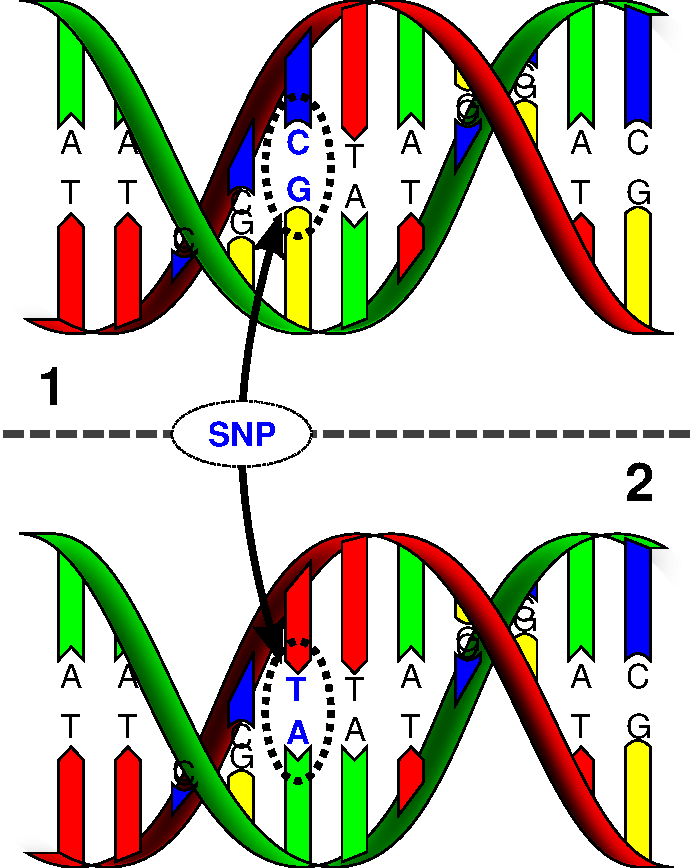
\includegraphics[width=0.4\textwidth]{bilder/DNA_SNP}
	\end{center}
	\caption[Visualisierung eines SNP. (aus \protect\url{http://commons.wikimedia.org/wiki/File:Dna-SNP.svg})]{Visualisierung eines SNP. (aus \protect\url{http://commons.wikimedia.org/wiki/File:Dna-SNP.svg})}
	\label{fig:bio:muta:snp}
\end{figure}
Im Mai 2014 waren in der \textit{dnSNP}, einer Datenbank des amerikanischen \textit{National Center for Biotechnologie Information} \citet{NCBI2014} 62.387.983 SNPs verzeichnet\footnote{Im Jahr 1999 waren erst 7000 SNPs öffentlich bekannt \citep{Brookes1999}}. Auf Grund dieser Vielzahl sind diese Varianten Ursache für die Unterschiede zwischen verschiedenen Menschen, bei beispielsweise Haut- und Haarfarbe oder Körpergröße und -form. Auch sind sie für die Empfänglichkeit von Krankheiten verantwortlich.

Da die Veränderungsrate bei $10^{-8}$ Änderungen pro Nucelotid und Generation liegt, sind einzelne Allele sind sehr stabil \citep{Brookes1999} \citep{Li1996}. 

Um die DNA eines Organismus überhaupt erstmal untersuchen zu können, muss diese sequenziert werden. Die Grundideen und verschiedene Arten der Sequenzierung werden im folgenden Abschnitt beschrieben.
\section{Sequenzierung}
\label{sec:bio:seq}
\marginpar{Jan}

Die Sequenzierung bezeichnet eine Methode zur Bestimmung der Nukleotid-Abfolge der untersuchten DNA. Seit 1977 wurden dabei verschiedene Methoden entwickelt, welche sich in Funktionsweise und Leistung deutlich unterscheiden. Die ersten entwickelten Verfahren waren dabei die chemische Methode von \textsc{Maxam} und \textsc{Gilbert} und die deutlich überlegendere Kettenabbruchmethode von \citet{Sanger1977}, welche nachfolgend vorgestellt wird. Alle weiteren Methoden, die zeitlich später entwickelt wurden, werden auch als \textbf{Next-Generation Sequencing} bezeichnet, von denen einige weitere im Verlauf dieses Kapitels vorgestellt werden.
\subsection{Kettenabbruchmethode}
\label{sec:bio:seq:kette}
\marginpar{Jan}

Die Kettenabruchmethode (auch als \textit{Dideoxy-Methode} bezeichnet) sequenziert eine eingebrachte DNA mittels Synthese durch eine Polymerase \citep{Jansohn2011}. 

Zur Vorbereitung muss die zu untersuchende DNA in hoher Stückzahl verfügbar sein. Die Klonierung erfolgt beispielsweise mit der in Abschnitt \ref{sec:bio:zell:pcr} vorgestellten Technik \textit{PCR}. Die Polymerase verlängert nun einen eingebrachten Primer, dessen Sequenz bekannt ist, so dass ein Komplement entsteht. In jedem Zyklus wird ein markiertes Nukleotid, ein sogenanntes \textit{Didesoxyribonukleosid-Triphosphat} (ddNTP), eingebracht. Diese besitzen am 3' Ende keine Hydroxygruppe. Da sich dort normalerweise die Verbindung zum nächsten Nukleotid befindet, kommt es beim Einbau eines ddNTP zum Abbruch der Kette und die Synthese terminiert.
\begin{figure}[htb]
	\begin{center}
		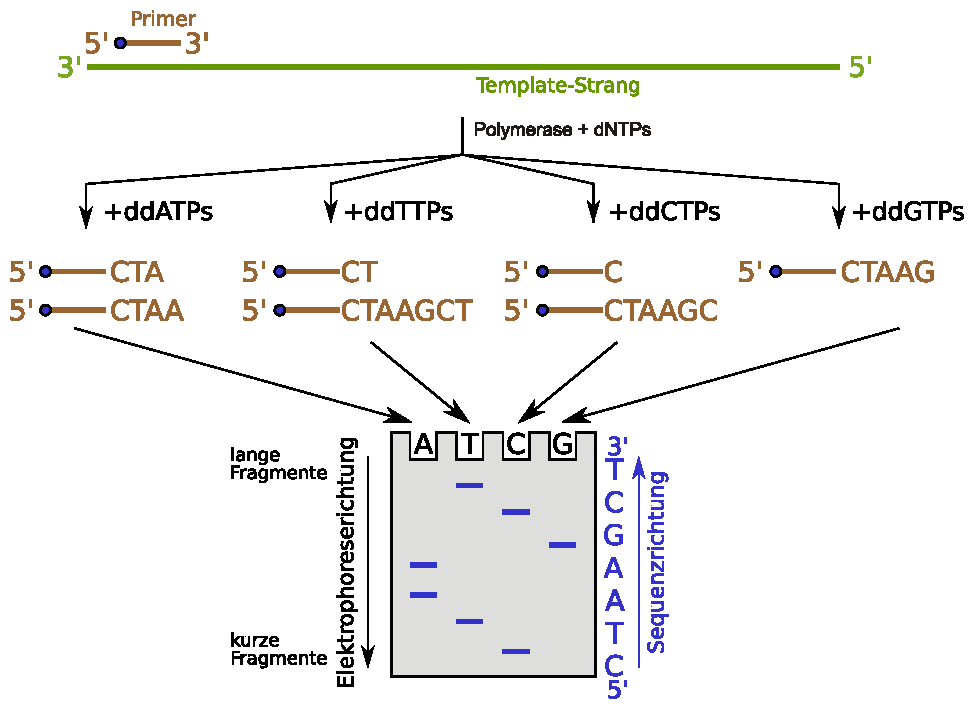
\includegraphics[width=0.6\textwidth]{bilder/Sequenzierung_Kettenabbruch}
	\end{center}
	\caption[Visualisierung der Kettenabbruchmethode nach Sanger. (aus \protect\url{http://commons.wikimedia.org/wiki/File:Didesoxy-Methode.svg})]{Visualisierung der Kettenabbruchmethode nach Sanger. (aus \protect\url{http://commons.wikimedia.org/wiki/File:Didesoxy-Methode.svg})}
	\label{fig:bio:seq:kette}
\end{figure}
Dadurch entsteht eine Vielzahl von DNA-Fragmenten mit unterschiedlichen Längen. Das Ablesen der Kodierung erfolgt in einer \textit{Elektrophorese}. Kurze Fragmente wandern, wie in Abbildung \ref{fig:bio:seq:kette} illustriert, am weitesten. Durch die Markierungen des jeweils letzten Nukleotids jedes Fragments lässt sich der genetische Code schrittweise erweitern. 

In der Vergangenheit nutzte man eine radioaktive Markierung der Nukleotide. Um das Gefahrenrisiko zu senken, wurden verschiedene fluoreszierende Markierungen verwendet %was sich vorteilhaft auf die Nutzung auswirkte?. 
Die entstehenden Reads besitzen eine Länge von bis zu 1000 Basenpaaren, dessen Sequenzierung Kosten in Höhe von $\$0{,}50$ pro Tauschend Basenpaaren verursachten. Auch wurde eine hohe Genauigkeit von bis zu $99{,}9 \%$ erzielt \citep{Shendure2008}. Leider ist die Kettenabbruchmethode aufwendig und kostet viel Zeit. Daher wurden neue Sequenziertechniken entwickelt, welche nachfolgend vorgestellt werden.
\newline
\subsection{Cyclic reversible termination (CRT)}
\label{sec:bio:seq:crt}
\marginpar{Jan}

Die Sequenziermethode \emph{CRT} (Cyclic reversible termination) nutzt ebenfalls einen Abbruch der Kette zur Nukleotidbestimmung aus. Im Gegensatz zur Methode von Sanger ist dieser Abbruch aber reversibel und benötigt keine Klonierung in hoher Anzahl. In jedem Zyklus wird versucht, genau ein farblich markiertes Nukleotid an den komplementären Strang der zu untersuchenden DNA zu binden. Der angesprochene \textit{reversible Terminator} unterbricht die Bindung von weiteren Molekülen. Nachdem die Fluoreszenz gemessen wurde und damit das gebundene Nukleotid identifiziert wurde, muss der fluoreszierende Terminator von der DNA gespalten werden, bevor der nächste Zyklus beginnt.

Wahlmöglichkeiten gibt es bei der Art der Markierung. Die erste Möglichkeit besteht darin, gleichzeitig alle vier verschiedenen Nukleotide hinzuzufügen, wobei jedes eine andere Fluorophore zur Identifikation erhält. Die andere Möglichkeit sieht für jedes Molekül denselben Farbstoff vor. In jedem Zyklus muss dabei darauf geachtet werden, dass ein anderes dNTP hinzugefügt wird, um die korrekte Sequenz ermitteln zu können. 

Die entstehenden Reads hatten bei Verwendung der ersten Maschinen dieser Plattform eine Länge von ca. 30 Basenpaaren, die neuen Modelle erreichen Längen von über 100 Basenpaaren \citep{Metzker2010}.
\subsection{Sequenzierung durch Hybridisierung}
\marginpar{Jan}

Diese Art der Sequenzierung nutzt den Umstand aus, dass sich passende DNA-Einzelstränge unter geeigneten Bedingungen zu einem komplementären Doppelstrang zusammensetzen. Zur Vorbereitung wird eine Vielzahl von DNA-Sonden, sogenannten \textit{Oligonukleotiden} mit einer bekannten Folge von 4 - 8 Nukleotiden, an einer festen Oberfläche befestigt \citep{Gresham2008}. Möglich ist auch die Nutzung von industriell gefertigten DNA-Chips. Die zu untersuchenden DNA-Abschnitte werden farblich markiert und hinzugefügt. Durch Untersuchung der Markierungen an den Positionen der Oligonukleotide kann entschieden werden, ob eine Bindung stattfand. Fällt das Ergebnis positiv aus, kann die Sequenz dieses Reads durch Komplementierung der Basenabfolge des jeweiligen Oligonukleotids bestimmt werden.
\subsection{Pyrosequezierung}
\label{sec:bio:seq:pyro}
\marginpar{Jan}

Das Grundvorgehen der Pyrosequenzierung ist die Beobachtung einer DNA-Replikation. Zur Vorbereitung werden die folgenden vier Enzyme zugegeben: DNA-Polymerase, ATP-Sulfurylase, Luciferase, Apyrase \citep{Ahmadian2006}. \\
Die eigentliche Sequenzierung läuft nun zyklenweise ab. Die Polymerase sucht ein freies Nukelotid, welches an den komplementären DNA-Strang andocken kann. Iterativ werden jeweils die Desoxyribonukleosidtriphosphate dATP, dCTP, dGTP, dTTP hinzugefügt. Kann ein Nukleotid andocken, wird durch die Polymerase \textit{Pyrophosphat} freigesetzt, welches dann durch ein weiteres Enzym, der ATP-Sulfurylase, zu \textit{Adenosintriphosphat (ATP)} umgewandelt wird. Die Luciferase, welche ursprünglich aus Glühwürmchen extrahiert wurde, katalysiert das ATP zu einem Lichtblitz \citep{Ahmadian2006}. Somit ist klar: Tritt ein Lichtblitz auf, konnte die Polymerase das aktuelle Nukleotid binden und bildet ein weiteres Glied der Sequenz. 
\begin{figure}[H]
	\begin{center}
		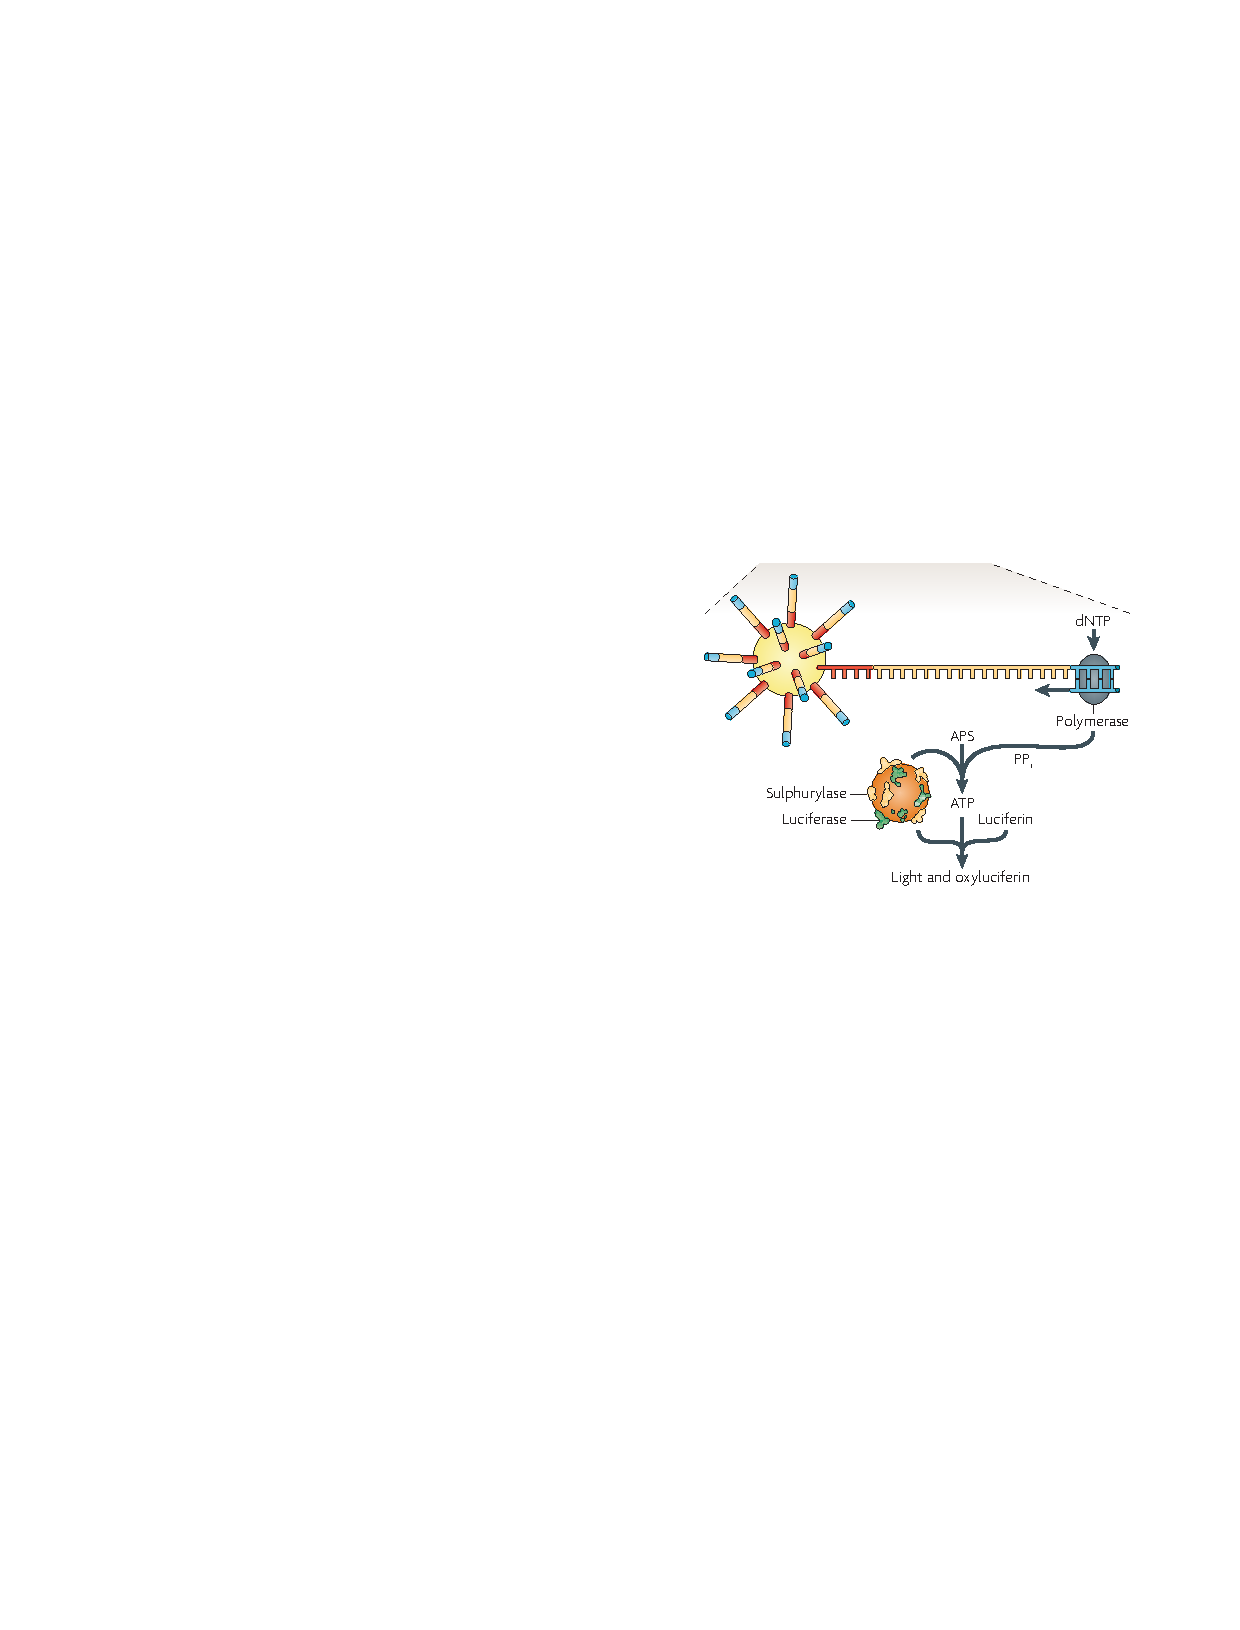
\includegraphics[width=0.6\textwidth]{bilder/Sequenzierung_Pyro_Schema}
	\end{center}
	\caption{Darstellung der Pyrosequenzierung (aus \citet{Metzker2010})}
	\label{fig:bio:seq:pyro:schema}
\end{figure}
Nach mehreren Zyklen und der Zugabe der verschiedenen dNTPs lässt sich der gesamte Read konstruieren. Die gesamte Beobachtung der Sequenzierung muss dabei in Echtzeit erfolgen, damit die Lichtblitze den richtigen dNTPs zugeordnet werden können \citep{Shendure2008}. Außerdem ist wichtig, dass auch die Intensität des Lichtblitzes gemessen wird, welche proportional zur Anzahl der eingebauten Nukleotide steigt. Für die Sequenz bedeutet dies, falls ein Lichtblitz mit doppelter Intensität auftritt, kommt das entsprechende Nukleotid zweimal vor. 
\begin{figure}[H]
	\begin{center}
		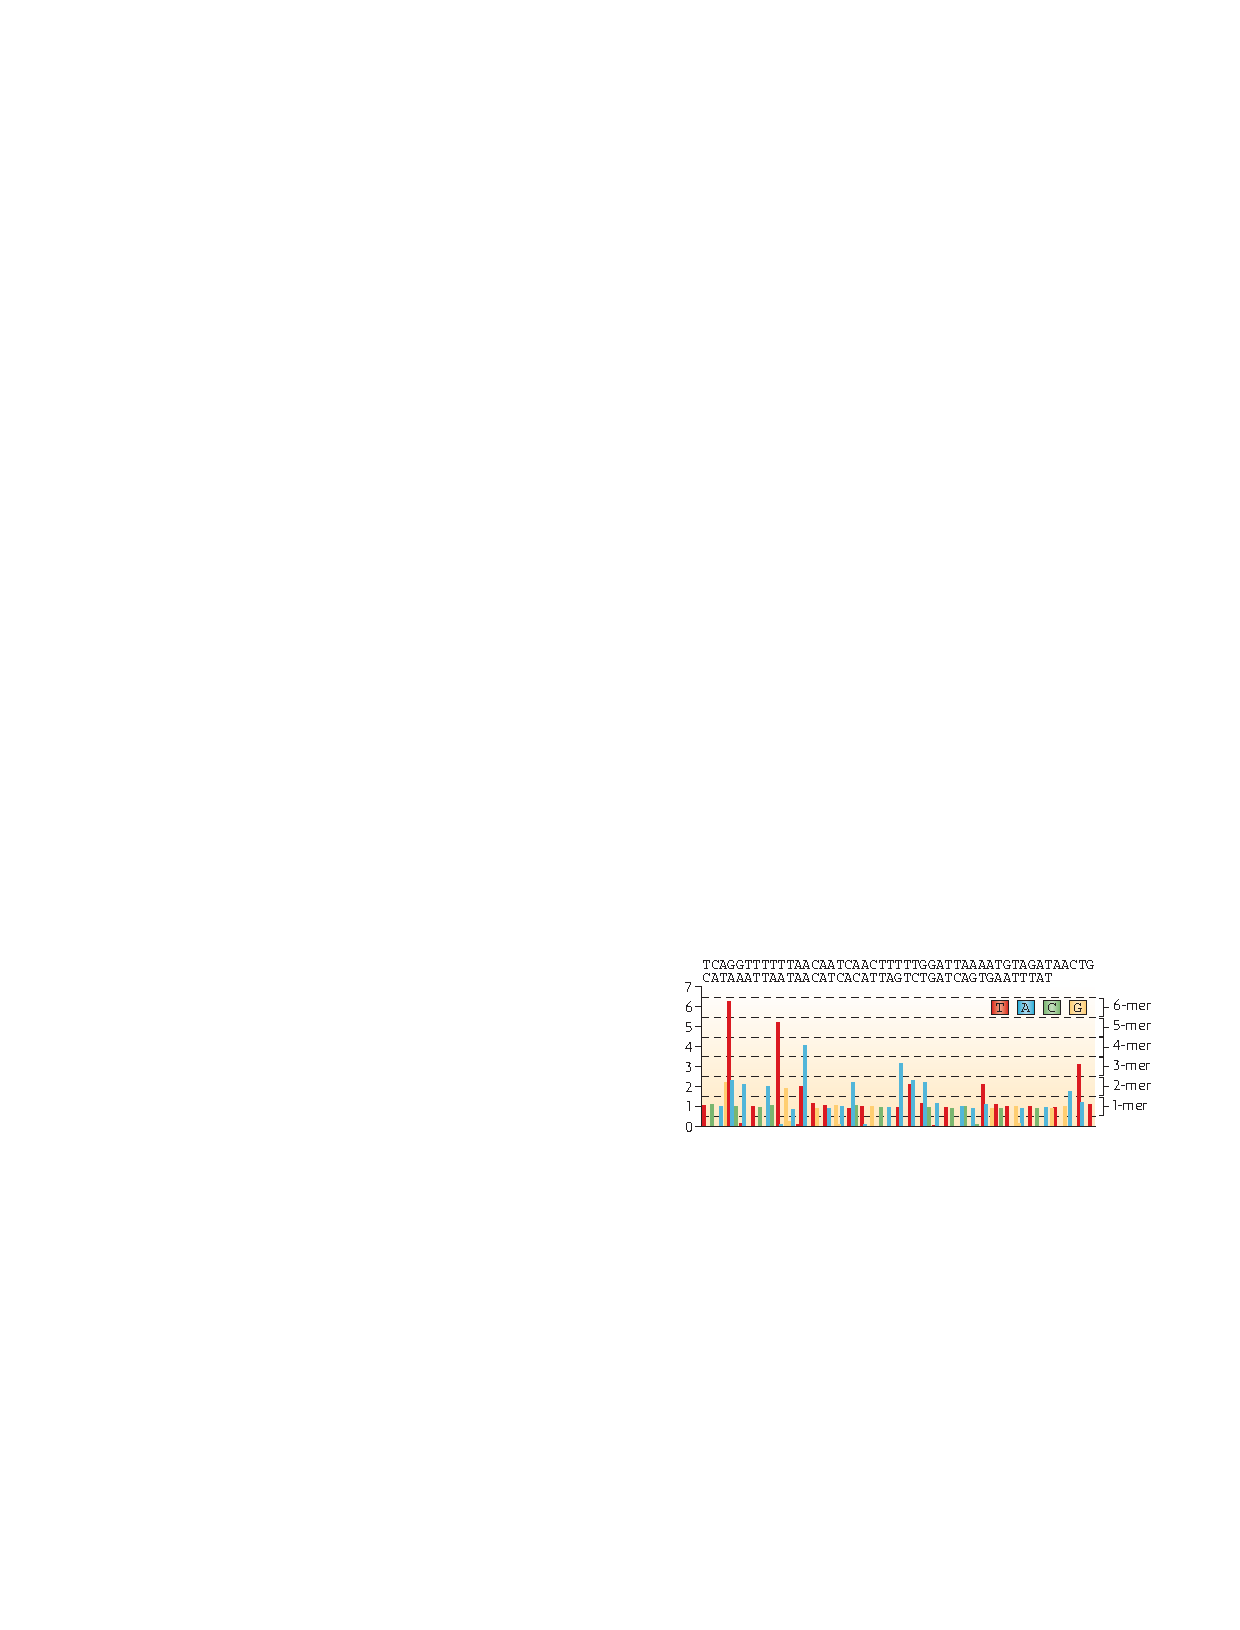
\includegraphics[width=0.8\textwidth]{bilder/Sequenzierung_Pyro_Diagramm}
	\end{center}
	\caption{Intensität der Lichtblitze (aus \citet{Metzker2010})}
	\label{fig:bio:seq:pyro:diagram}
\end{figure}
Ein großer Vorteil der Pyrosequenzierung ist die hochparallele Generierung von hunderttausenden Reads mit einer Länge von bis zu 400 Basenpaaren. Auch ist es möglich, dass verschiedene Proben gleichzeitig analysiert werden können, was sich kostensenkend auswirkt \citep{Siqueira2012}. Durch die langen Reads ist eine zuverlässige Erkennung von SNPs möglich, jedoch ist die Fehlerrate bei der Erkennung von Indels hoch, da \textit{Homopolymere}, also Wiederholungsfolgen derselben Base, nur anhand der verschiedenen Intensität der Lichtblitze erkannt werden können \citep{Shendure2008}.
\subsection{Echtzeit-Sequenzierung}
\label{sec:bio:seq:realtime}
\marginpar{Jan}

Bei der Echtzeit-Sequenzierung kann die ermittelte DNA-Sequenz direkt durch Beobachtung der Polymerase abgelesen werden. Im Gegensatz zur Pyrosequenzierung, welche ebenfalls in Echtzeit beobachtet werden muss, muss bei diesem Ansatz die DNA-Synthese nicht gestoppt werden. Einzelne Polymerasen werden an der Oberfläche eines Detektors angebracht, der Nukleotide erkennen kann, die um ein fluoreszierendes Phosphat erweitert wurden\citep{Eid2009}. Diese werden in hoher Anzahl hinzugegeben. In jedem Zyklus wird versucht, eines der Nukleotide einzubinden. Ist der Versuch erfolgreich, löst sich das farblich markierte Pyrophosphat und löst einen messbaren Puls aus. Der Detektor misst diesen und setzt daraus die Sequenz zusammen.
\begin{figure}[H]
	\begin{center}
		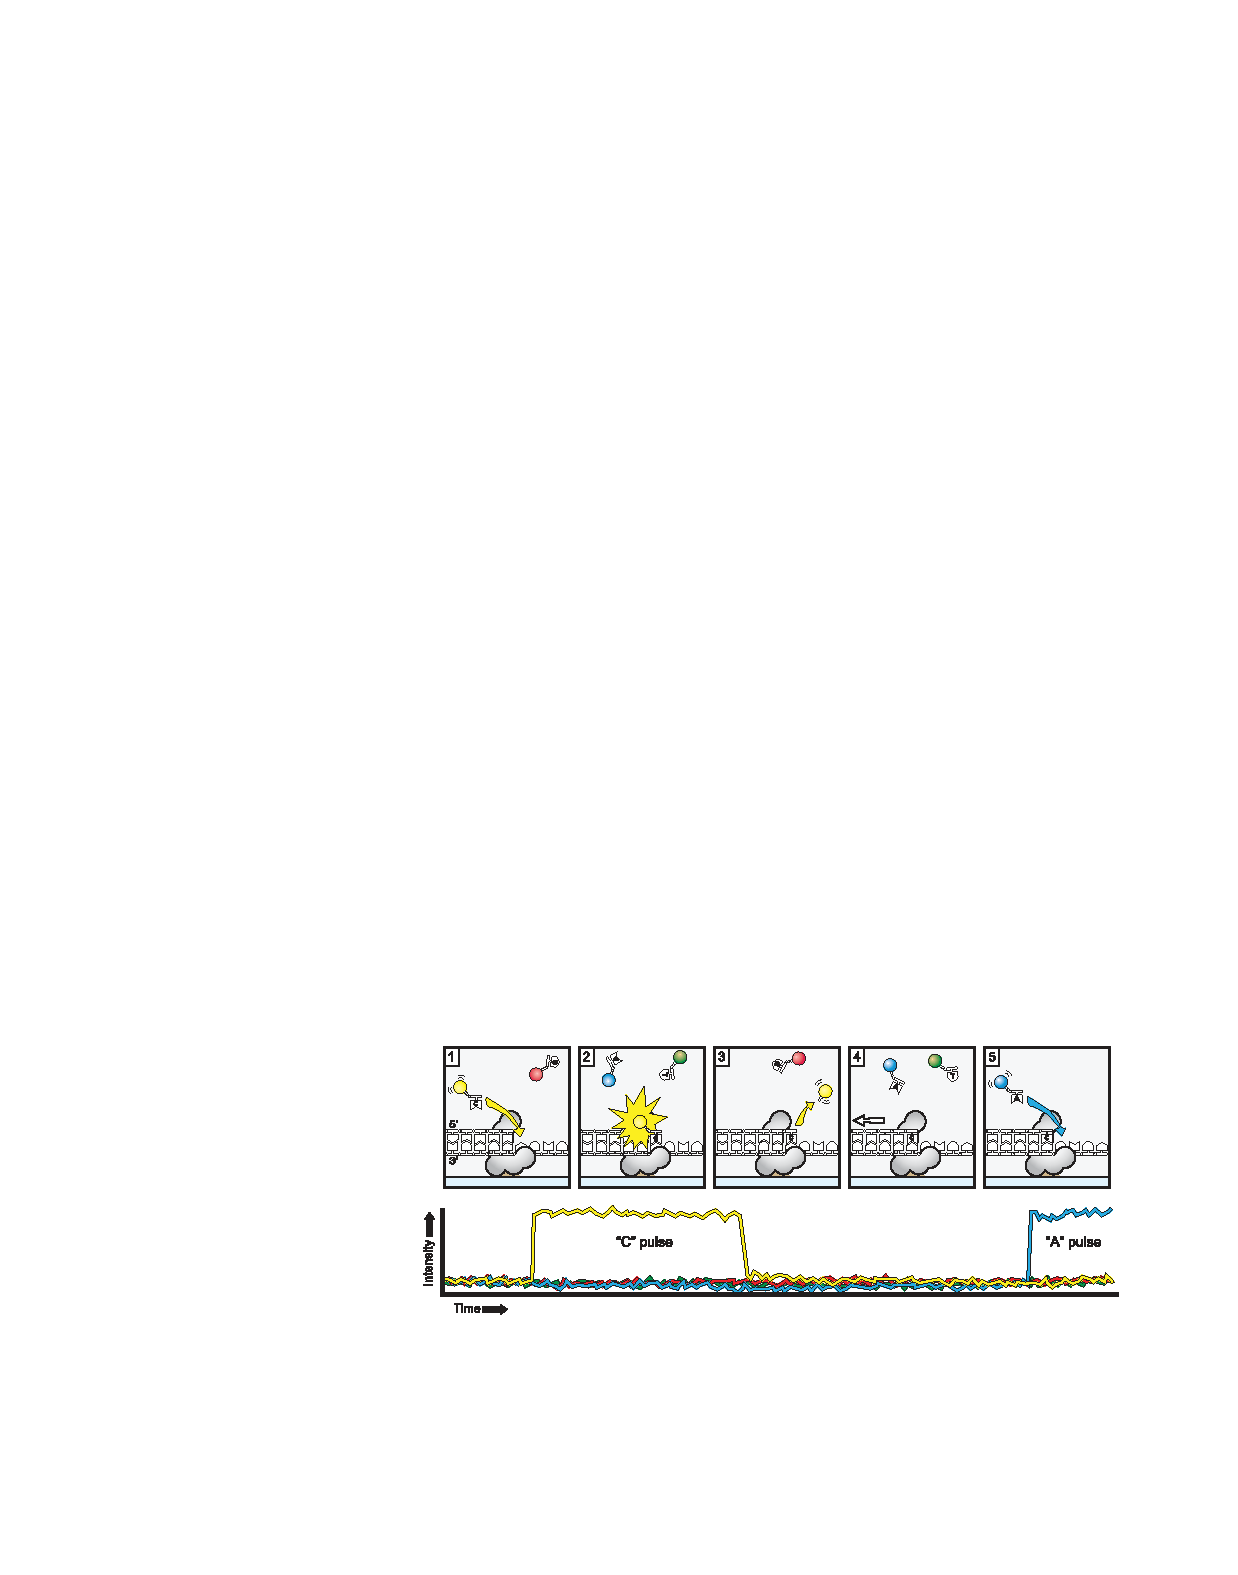
\includegraphics[width=\textwidth]{bilder/Sequenzierung_Realtime}
	\end{center}
	\caption{Darstellung der Echtzeitsequenzierung (aus \citet{Eid2009})}
	\label{fig:bio:seq:realtime}
\end{figure}
	Vorteilhaft wirken sich hohe Readlängen von bis zu 1000 Basenpaaren und die hohe Geschwindigkeit der Sequenzierung aus, welche nur von der Synthesegeschwindigkeit\footnote{Diese Geschwindigkeiten liegen zwischen $0.7$ und $1.5$ Basen pro Sekunde \citep{Eid2009}.} der verwendeten Polymerase abhängig ist \citep{Metzker2010}. Die Genauigkeit eines einzelnen Sequenzierungsdurchgangs ist relativ ungenau ($\sim 83\%$). Durch mehrfache Wiederholung der Sequenzierung desselben Reads lässt sich diese Genauigkeit auf über $99\%$ erhöhen \citep{Eid2009}.

\chapter{Statistiken}
\label{sec:stats}
\marginpar{Jens}

In diesem Kapitel werden einige Statistiken über die Verteilung der bekannten Varianten des Humangenoms vorgestellt. Warum wir diese Statistiken erstellt haben, soll der folgende Abschnitt klären:

\section{Motivation}
\label{sec:stats:motivation}
\marginpar{Jens}
Die Aufgabe unserer Projektgruppe ist es, einen Readmapper zu implementieren, der nach Möglichkeit bekannte Varianten direkt unterstützt. Beispielsweise könnte an einer bestimmten Position im Referenzgenom die Base Adenin stehen. Es ist aber bekannt, dass an dieser Position auch häufig Thymin vorkommt. Ein Read, der zu jenem Bereich im Referenzgenom passt, enthält möglicherweise an besagten Stelle diese Variante (also Thymin statt Adenin). Beim Readmapping sollte dieser Basenunterschied zwischen Referenzgenom und Read jedoch nicht als Fehler gewertet, da es sich hierbei um eine häufige Variante handelt. Diese Variantentoleranz wird von vielen Readmappern nicht unterstützt. Da die Anzahl der bekannten Varianten jedoch stetig zunimmt, wäre eine direkte Unterstützung der Varianten beim Readmapping sehr wünschenswert.

Als Grundlage für viele Readmapper werden $q$-Gramme verwendet. Im Allgemeinen ist ein $q$-Gramm ein Teilstring eines Textes bestehend aus $q$ Fragmenten. Fragmente können die Buchstaben eines Textes sein, aber auch Silben oder ganze Wörter, sofern es sich sprachliche Texte handelt. In unserem Fall stellt das Referenzgenom zusammen mit den Reads den Text dar. Die Fragmente sind die vier möglichen Basen (A, C, G und T). Um Reads im Referenzgenom zu finden, wird das Referenzgenom und die Reads in ihre $q$-Gramme zerlegt. Kommen in einem Abschnitt des Referenzgenoms viele $q$-Gramme vor, die auch in einem bestimmten Read vorhanden sind, so ist die Wahrscheinlichkeit hoch, dass dieser Read zu jener Stelle im Referenzgenom passt. Durch die Verwendung der $q$-Gramme erhalten wir eine gewisse Fehlertoleranz: Enthält ein Read einen Sequenzierfehler, so ist nur ein Teil seiner $q$-Gramme davon betroffen. Das heißt, wir können den Read immer noch im Referenzgenom wiederfinden. 

An dieser Stelle ist es hilfreich, eine Vorstellung über die Größenordnungen zu bekommen: Das Humangenom besteht wie bereit erwähnt aus 3 Milliarden Basenpaaren. Reads der zweiten Sequenzier-Generationen haben in der Regel eine Länge von 101 Basenpaaren. Als $q$-Gramm-Länge werden meist Werte zwischen 8 und 24 verwendet. Hier müssen Experimente zeigen, bei welcher $q$-Gramm-Länge die besten Ergebnisse erzielt werden. Bei dem sehr schnellen Readmapper PEANUT (ParallEl AligNment UTility)
) \citep{Koester2014} haben die $q$-Gramme beispielsweise eine feste Länge von 16 Basen. Bei sehr langen $q$-Grammen leidet die Fehlertoleranz, da von einem Fehler bereits sehr viele $q$-Gramme betroffen sind. Sind die $q$-Gramme zu kurz, wird der Read möglicherweise an eine falsche Stelle gemappt, da die $q$-Gramme den Read nicht ausreichend repräsentieren. Zur Zeit (2014) sind etwa 60 Millionen Varianten bekannt.

Damit die Suche hinreichend schnell ist, wird mit den $q$-Grammen des Textes ein Suchindex aufgebaut. Wie dieser genau funktioniert, hängt von dem verwendeten Algorithmus ab und ist an dieser Stelle erstmal nicht wichtig. In Kapitel \ref{sec:lsh} erklären wir detailliert den in unserer Implementierung verwenden Suchindex. 

Wie kann man nun mit Hilfe der $q$-Gramme eine Variantentoleranz erzielen? Die einfachste Möglichkeit ist, die Varianten hinten an der Referenzgenom anzuhängen. Bei SNPs (Veränderung einer Base, vgl. Abschnitt \ref{sec:bio:muta:gen}) kann aber geschickter vorgegangen werden: Liegt an einer Position in einem $q$-Gramm eine Variante vor, so fügt man beide Möglichkeiten zum Such-Index hinzu. Dieses Vorgehen ist jedoch problematisch, wenn viele Varianten in einen $q$-Gramm vorkommen, da man alle Kombinationen zum Suchindex hinzufügen müsste. Im Extremfall gäbe es an allen $q$ Positionen des $q$-Gramms eine Variante, sodass sich $2^q$ Kombinationen ergeben würden. 

Hier stellt sich die Frage, wie die Varianten verteilt sind. Kommen die Varianten gleichverteilt vor? Oder gibt es Abschnitte mit sehr vielen Varianten? Im ersten Fall käme eine Variante nur alle 50 Basenpaare. Im letzteren Fall hätten wir das Problem der kombinatorischen Explosion. Um diese Fragen zu beantworten haben wir verschiedene Statistiken zur Verteilung der Varianten erstellt.

\section{Durchführung}
\label{sec:stats:durchfuhrung}
\marginpar{Jens}

Als Datengrundlage dienen die von der NCBI (National Center for Biotechnology Information) veröffentlichten Varianten des Humangenoms\footnote{
\url{ftp://ftp.ncbi.nih.gov/snp/organisms/human_9606_b141_GRCh37p13/VCF/}
}. Die zur Zeit bekannten Varianten sind das Ergebnis des 1000-Genome-Projekts\footnote{
\url{http://www.1000genomes.org/}
}, bei dem die DNA von über 1000 Menschen sequenziert wurde. Für unsere Statistiken haben wir auf zwei Varianten-Dateien zurückgegriffen. Die eine Datei 
(\glqq 00-All.vcf\grqq )
enthält alle bekannten Varianten, die andere Datei 
(\glqq common\_all.vcf\grqq )
nur jene, die bei mindestens 1\% der Individuen vorkommen. Die Menge dieser Varianten wird im folgenden als \emph{häufige Varianten} bezeichnet.
\newpage

\section{Ergebnisse und Auswertung} 
\label{sec:stats:res}
\marginpar{Jens}

Im Laufe unserer Projektgruppe haben wir viele verschiedene Statistiken erstellt. Die wichtigen und aussagekräftigsten sollen im Folgenden vorgestellt und analysiert werden: 

\subsection{Allgemeine Statistiken}
\label{sec:stats:res:allg}
\marginpar{Jens}

Zunächst ein paar allgemeine Informationen über die beiden Varianten-Dateien: Bisher sind etwa 63 Millionen Varianten bekannt, 85\% davon sind SNPs, die restlichen 15\% sind Indels. Circa die Hälfte dieser Varianten (28 Millionen) kommen bei mindestens 1\% der Individuen vor. Bei diesen häufigen Varianten handelt es sich hauptsächlich um SNPs (95\%). Nur 5\% der häufigen Varianten sind Insertionen oder Deletionen. 

\subsection{Anzahl der SNPs in einem $q$-Gram}
\label{sec:stats:res:variantsq16}
\marginpar{Jens}

Im Abschnitt \ref{sec:stats:motivation} kam bereit die Frage auf, wie die Varianten verteilt sind. Insbesondere ist interessant, ob es $q$-Gramme gibt, bei denen an vielen oder fast allen Stellen SNPs vorkommen. Das Diagramm in Abbildung \ref{fig:stats:variantsq16} zeigt, wie häufig $x$ SNPs in einem $q$-Gramm der Länge 16 vorkommen. Die konstante Länge von 16 wurde gewählt, da sich diese bei PEANUT-Algorithmus etabliert hat.

\begin{figure}[h]
\pgfplotsset{footnotesize,width=12cm,compat=1.8}
%\pgfplotsset{footnotesize,samples=10}
\begin{center}
\begin{tikzpicture}
\begin{semilogyaxis}[%restrict y to domain=0:5e10,
xmin=0,xmax=16,
xlabel=Anzahl der SNPs,
ylabel=Häufigkeit,
title={Anzahl von SNPs in 16-Grammen},
legend pos=outer north east,
scaled ticks=false,
ymajorgrids=true,
xmajorgrids=true,
legend columns=-1,
legend entries={Alle Varianten, Häufige Varianten},
legend to name=leg:variantsq16
]
\addplot[mark=x, thick, color=red, smooth] table[x=n,y=all] {data/variants_Q16_snp.dat};
\addplot[mark=*, thick, color=blue, smooth] table[x=n,y=common] {data/variants_Q16_snp.dat};
\end{semilogyaxis}
\end{tikzpicture}
\ref*{leg:variantsq16}
\end{center}
\caption{Anzahl von SNPs in $q$-Grammen der Länge 16.}
\label{fig:stats:variantsq16}
\end{figure}

Berücksichtigt man alle Varianten (rote Kurve), so stellt man fest, dass es etwa 5000 $q$-Gramme gibt, bei denen an allen Stellen eine Variante vorkommt. Obwohl die Datei mit den häufigen Varianten nur halb so viele Varianten enthält, sind extreme Variantenhäufungen hier deutlich seltener (siehe blaue Kurve). 16-Gramme mit 11 oder mehr Varianten kommen beispielsweise gar nicht mehr vor.

Man kann also davon ausgehen, dass das Risiko der kombinatorischen Explosion bei ausschließlicher Verwendung der häufigen Varianten deutlich geringer ist als bei Verwendung aller Varianten. 

Das Diagramm \ref{fig:stats:variantsq16} zeigt jedoch nicht wie viele Varianten pro Position vorkommen. Dies ist aber durchaus relevant. Existiert an jeder Position eines 16-Gramms genau eine Variante, so gäbe es bei einem 16-Gramm mit 16 SNPs $2^{16} = 65536$ Kombinationen, die zum Suchindex hinzugefügt werden müssten. Das ist bereits eine große Menge von $q$-Grammen, aber angesichts der Tatsache, dass das Humangenom ohne Varianten circa 3 Milliarden $q$-Gramme enthält, könnte man mit diesen 65535 zusätzlichen $q$-Grammen durchaus noch zurechtkommen. Kann jedoch an jeder Position des 16-Gramms jede Base stehen (d.h. wir haben drei Varianten pro Basenpaar), dann gibt es $4^{16} \approx 4,3 \cdot 10^9$ Kombinationen. Damit würden sich die Menge der $q$-Gramme im Suchindex mehr als verdoppeln\footnote{Dieser Fall ist etwas künstlich, da man an solch eine Position jeden Read mappen könnte.}.

Um genauere Aussagen zu treffen, wäre es daher sinnvoll die tatsächliche Anzahl der Kombinationen zu zählen. %Darüber hinaus wäre es interessant, andere $q$-Grammlängen zu betrachten. 

\subsection{Kombinatorische Explosion}
\label{sec:stats:res:explosion}
\marginpar{Jens}

Um einen $q$-Gramm-basierten Suchindex variantentolerant zu machen, könnte man alle $q$-Gramme betrachten, die sich aus Kombinationen der verschiedenen bekannten SNPs ergeben. Dabei stellt sich die Frage, wie viele $q$-Gramme dann dem Suchindex hinzugefügt werden müssten. In Diagramm \ref{fig:stats:explosion} ist genau dies dargestellt: Die $y$-Achse zeigt die Anzahl der $q$-Gramme in Abhängigkeit von der $q$-Grammlänge auf der $x$-Achse. 

\begin{figure}[h]
\pgfplotsset{footnotesize,width=12cm,compat=1.8}
%\pgfplotsset{footnotesize,samples=10}
\begin{center}
\begin{tikzpicture}
\begin{axis}[restrict y to domain=0:5e10,
xmin=0,xmax=32,
ymin=1e9,ymax=1e10,
xlabel=$q$-Grammlänge,
ylabel=Anzahl der Kombinationen,
title={Kombinatorische Explosion (SNPs)},
legend pos=outer north east,
scaled ticks=false,
ytick={1e9,2e9,3e9,4e9,5e9,6e9,7e9,8e9,9e9,10e9},
xtick={0,2,...,32},
minor x tick num=1,
ymajorgrids=true,
xmajorgrids=true,
legend columns=-1,
legend entries={Kein Limit, Limit = 65536, Limit = 16, Nur häufige Varianten (kein Limit)},
legend to name=leg:explosion
]
\addplot[thick, color=red, smooth] table[x=q,y=nolimit] {data/combinations_snp_all.dat};
\addplot[thick, color=blue, smooth] table[x=q,y=65536] {data/combinations_snp_all.dat};
\addplot[thick, color=green, smooth] table[x=q,y=16] {data/combinations_snp_all.dat};
\addplot[thick, color=black, smooth] table[x=q,y=nolimit] {data/combinations_snp_common.dat};
%\legend{Kein Limit, Limit = 65536, Limit = 16, Nur häufige Varianten (kein Limit)};
\end{axis}
\end{tikzpicture}
\ref*{leg:explosion}
\end{center}
\caption{Anzahl der $q$-Gramme, die zum Suchindex hinzugefügt werden müssen, wenn alle SNP-Kombinationen berücksichtigt werden.}
\label{fig:stats:explosion}
\end{figure}

Ohne weitere Beschränkungen (rote Kurve) kommt es zur der bereits oben befürchteten kombinatorischen Explosion: Bei $q=10$ müssten etwa 5 Milliarden $q$-Gramme hinzugefügt werden, also 66\% mehr als ohne Variantenberücksichtigung. Bei $q=11$ hat sich die $q$-Grammlänge bereits verdreifacht. Bei $q=16$ lägen wir bei 2,17 Billionen $q$-Grammen, also circa Faktor 700 mehr. Diese extrem hohen Zahlen werden dadurch verursacht, dass an einigen Stellen sehr viele Varianten vorkommen. Es gibt $16$-Gramme im Referenzgenom bei denen an allen Stellen mindestens zwei SNPs vorkommen. Damit erzeugt solch ein $16$-Gramm über $3^{16} \approx 43 \cdot 10^6$ Varianten. An solch eine Stelle könnte man äußerst viele Reads mappen, indem einfach die passenden Varianten gewählt werden. Es macht also eigentlich keinen Sinn, jede dieser Kombinationen zum Suchindex hinzuzufügen.

Aus diesem Grund kamen wir auf die Idee, die Anzahl der Kombinationen pro $q$-Gramm im Genom zu beschränken. Die blaue Kurve zeigt das Ergebnis bei einer Beschränkung (Limit) von 65536 Kombinationen. Gibt es $q$-Gramme mit mehr Kombinationen, würde man nur 65536 von diesen zum Suchindex hinzufügen. Obwohl dieser Wert relativ groß ist, kann dadurch die kombinatorische Explosion vermieden werden. Welche Kombinationen dabei verwendet werden, ist an dieser Stelle nicht wichtig, aber durchaus eine interessante Frage. Bei $q=16$ erhalten wir etwa 6 Milliarden $q$-Gramme, also doppelt so viel wie ohne Berücksichtigung der Varianten. Dieser Wert ist gut beherrschbar. Reduziert man das Limit weiter auf 16, ergeben sich etwa 4 Milliarden $q$-Gramme, also nochmal deutlich weniger.

Besonders interessant ist die schwarze Kurve, bei der nur die häufigen Varianten berücksichtigt wurden. Bei $16$-Grammen erhalten wird gerade einmal 3,5 Milliarden Kombinationen, obwohl es keine Beschränkung der Anzahl der Kombinationen in einem $q$-Gramm gibt. 
Wenn also nur die häufigen Varianten berücksichtigt werden, kann auf die Implementierung eines Limit verzichtet werden, da sich die Gesamtanzahl der $q$-Gramme im Suchindex nicht wesentlich erhöht. Trotzdem könnte eine Beschränkung der Kombinationsanzahl sinnvoll sein: Treten viele Varianten in einen $q$-Gramm auf, so können deutlich mehr Reads an diese Position gemappt werden als an Stellen des Humangenoms an denen keine Varianten vorkommen. Das heißt variantenreiche Stellen werden beim Readmapping bevorzugt, wenn starke Variantenhäufungen vorkommen.

\subsection{Länge von Sequenzen mit vielen Varianten}
\label{sec:stats:res:nogapseq}
\marginpar{Jens}

Bisher haben wir uns nur mit der Verteilung von SNPs beschäftigt. Im folgenden betrachten wir die Verteilung aller Varianten, also SNPs und Indels. Das Diagramm in Abbildung \ref{fig:stats:nogapseq} zeigt die Häufigkeit von Sequenzen bestimmter Länge, bei denen an allen Positionen Varianten vorkommen. Auf der x-Achse ist die Länge der Variantensequenz aufgetragen und auf der y-Achse die Häufigkeit in der jeweiligen Varianten-Datei. Bei der Berechnung des Diagramms wurden ab einer Länge von 12 Basenpaaren mehrere Werte auf der x-Achse zusammengefasst, um eine Glättung der Kurve zu erzielen. Dem entsprechend können auch Häufigkeiten kleiner als 1 auftreten. Beispielsweise hat die rote Kurve im Bereich von 90 bis 100 Basenpaaren einen y-Wert von etwa 0,5. Dementsprechend gibt es $0{,}5 \cdot (100 - 90) = 5$ Sequenzen mit einer Länge zwischen 90 und 100 Basenpaaren, bei denen an allen Positionen Varianten vorkommen können. Bei den beiden roten Kurven wurden als Datengrundlage alle Varianten verwendet, bei den beiden blauen Kurven nur die häufigen Varianten. Bei den gestrichelten Kurven darf zwischen den Varianten eine Lücke von maximal vier variantenlosen Positionen des Referenzgenoms vorkommen, ohne dass dies als neue Variantensequenz gezählt wird. Die x-Achse zeigt dabei nicht die Länge der Variantensequenz, sondern die Anzahl der Positionen, an denen Varianten vorkommen können.

\begin{figure}[h]
\pgfplotsset{footnotesize,width=12cm,compat=1.8}
%\pgfplotsset{footnotesize,samples=10}
\begin{center}
\begin{tikzpicture}
\begin{loglogaxis}[%restrict y to domain=1e-10:1e10, log origin y=infty,
xmin=1,xmax=300,
ymin=1e-1,ymax=1e9,
xlabel=Anzahl der Varianten,
ylabel=Häufigkeit,
title={Länge von Sequenzen mit vielen Varianten},
legend pos=outer north east,
scaled ticks=false,
%ytick={1e9,2e9,3e9,4e9,5e9,6e9,7e9,8e9,9e9,10e9},
%xtick={0,2,...,32},
%minor x tick num=1,
ymajorgrids=true,
xmajorgrids=true,
%xminorgirds=true,
legend columns=2,
legend entries={Alle Varianten (keine Lücke), Alle Varianten (4er Lücke), Häufige Varianten (keine Lücke), Häufige Varianten (4er Lücke)},
legend to name=leg:nogapseq
]
\addplot[thick, color=red, smooth] table[x=data,y=gap0] {data/nogapseq_both_all.dat};
\addplot[thick, color=red, smooth, densely dashed] table[x=data,y=gap4] {data/nogapseq_both_all.dat};
\addplot[thick, color=blue, smooth] table[x=data,y=gap0] {data/nogapseq_both_common.dat};
\addplot[thick, color=blue, smooth, densely dashed] table[x=data,y=gap4] {data/nogapseq_both_common.dat};
\end{loglogaxis}
\end{tikzpicture}
\ref*{leg:nogapseq}
\end{center}
\caption{Länge von Sequenzen mit Varianten an allen Positionen. Bei den gestrichelten Kurven dürfen zwischen zwei Varianten vier variantenlose Positionen stehen, ohne dass dies als neue Sequenz gewertet wird.}
\label{fig:stats:nogapseq}
\end{figure}

Wie auch im vorherigen Abschnitt fällt auf, dass starke Variantenhäufungen nur bei Verwendung aller bekannten Varianten vorkommen. Unter den häufigen Varianten besteht die längste lückenlose Variantensequenz gerade mal aus acht Basenpaaren. Im Gegensatz dazu gibt es bei Berücksichtigung aller Varianten noch Fälle mit 100 und mehr aufeinander folgenden Positionen, bei denen überall bekannte Varianten existieren. Selbst wenn man eine Lücke von bis zu vier variantenlosen Positionen zulässt, erhöht sich die Variantenanzahl der längsten Variantensequenz unter den häufigen Varianten gerade einmal auf 15. 

Das Diagramm zeigt nur Variantensequenzen mit einer Länge von maximal 300 Positionen. Ein Blick auf die Rohdaten zeigt aber, dass es sogar eine lückenlose Variantensequenz mit einer Länge zwischen 334 und 368 Positionen im Referenzgenom gibt. Lässt man eine Lücke von vier variantenlosen Positionen zu, ergibt sich sogar noch ein Eintrag bei über 5000 Varianten. 

Wir können also festhalten, dass es Stellen im Humangenom gibt, die bei den einzelnen Individuen sehr unterschiedlich aussehen. Unter den häufigen Varianten, die bei mindestens 1\% der Menschen existieren, kommen solche starken Variantenhäufungen nicht vor. Wir hatten bereits erwähnt, dass beim Zuordnen eines Reads zu einer ungefähren Position im Humangenom die Verwendung der häufigen Varianten sinnvoll ist. 

Auch bei der Berechnung des exakten Alignments (siehe Kapitel \ref{sec:align}) eines Reads an das Humangenom macht es Sinn, nur die häufigen Varianten zu verwenden. Denn an einer sehr variantenreichen Stelle würde das Alignment sonst vermutlich Variantenkombinationen verwenden, die bei keinem Individuum vorkommen. Alternativ könnte man auch dynamisch entscheiden, welche Varianten-Datei verwendet wird. Liegt an jener Stelle eine starke Variantenhäufung vor, so verwendet man nur die häufigen Varianten für das Alignment. Liegen nur wenige Varianten an jener Stelle vor, kann man auch gefahrlos auf alle Varianten zurückgreifen.

\subsection{Variantenhäufungen}
\label{sec:stats:res:manyvariants}
\marginpar{Jens}

Für interessierte Leser, die selbst weiter nachforschen wollen, zeigt die Tabelle \ref{tab:stats:manyvariants} die Chromosomen und Positionen von Stellen im Humangenom, bei denen viele Varianten vorkommen. \glqq Viele\grqq\ wurde dabei so definiert, dass in einem Fenster mit einer Breite von 2000 Basenpaaren mindestens 1000 Varianten vorkommen müssen. Die innerhalb der Projektgruppe geäußerte Vermutung, dass die Variantenhäufungen möglicherweise nur am Anfang oder am Ende eines Chromosoms vorkommen, kann die Tabelle eindeutig widerlegen.

\begin{table}[hp]
\begin{center}
\begin{tabular}{|r|r|r|r|}
\hline
\textbf{Chromosom} & \textbf{Position} & \textbf{Längen} & \textbf{Varianten} \\
\hline
1 & 43297968 & 3383 & 1560 \\
1 & 121483203 & 2854 & 1154 \\
1 & 207511977 & 22815 & 17703 \\
1 & 207669174 & 11066 & 7732 \\
1 & 207792710 & 3570 & 1678 \\
1 & 207804914 & 4556 & 2392 \\
2 & 127413243 & 30798 & 21454 \\
2 & 127443578 & 2000 & 1000 \\
2 & 127443580 & 5055 & 2767 \\
6 & 10532526 & 54184 & 37545 \\
6 & 32628205 & 2816 & 1159 \\
6 & 32630860 & 4510 & 2493 \\
6 & 58775341 & 4660 & 2434 \\
7 & 61967275 & 4090 & 2088 \\
16 & 46388873 & 5233 & 3089 \\
16 & 46393109 & 2001 & 1000 \\
16 & 46393113 & 3580 & 1718 \\
16 & 46403046 & 4835 & 2506 \\
19 & 569895 & 2873 & 1183 \\
X & 2707159 & 6025 & 3452 \\
X & 2714790 & 12269 & 7971 \\
Y & 2600930 & 5929 & 3362 \\
\hline
\end{tabular}
\end{center}
\caption{Sequenzen im Humangenom mit vielen Varianten (mindestens 1000 Varianten in einem Fenster mit einer Breite von 2000 Basenpaaren).}
\label{tab:stats:manyvariants}
\end{table}

Das Balkendiagramm in Abbildung \ref{fig:stats:examplewindow} zeigt ein Beispiel für einen Bereich mit besonders vielen Varianten im sechsten Chromosom. An jeder Position des 201 Basenpaare langen Fensters können Varianten vorkommen. Dabei sind SNPs in blau und Indels in rot dargestellt. Es fällt auf, dass an vielen Positionen drei SNP-Varianten vorkommen, d.h. hier kann jede der vier Basen (A, C, G und T) stehen. Stellen, an denen es nur eine SNP-Variante gibt, sind klar in der Minderheit. Der gezeigte Bereich verdeutlicht nochmals, dass die Verwendung aller bekannten Varianten beim Readmapping an manchen Stellen im Humangenom nicht sinnvoll ist.

\begin{figure}[hp]
\pgfplotsset{footnotesize,width=14cm,height=8cm,compat=1.8}
%\pgfplotsset{footnotesize,samples=10}
\begin{center}
\begin{tikzpicture}
\begin{axis}[%restrict y to domain=1e-10:1e10, log origin y=infty,
ybar,
xmin=-.5,xmax=200.5,
ymin=0,ymax=4,
xlabel=Position,
ylabel=Anzahl der Varianten,
title={Beispiel-Fenster für eine starke Variantenhäufung},
legend pos=north west,
scaled ticks=false,
ytick={0,1,2,3,4},
xtick={0,20,...,200},
minor x tick num=9,
ymajorgrids=true,
%xmajorgrids=true,
%xminorgirds=true,
bar width=.75,%.5,
%line width=0pt,
legend columns=1,%-1,
legend entries={SNPs, Indels},
%legend to name=leg:examplewindow
]
\addplot[fill, color=blue, draw opacity=0,bar shift=-.25] table[x=pos,y=snps] {data/exampleWindow.dat};
\addplot[fill, color=red, draw opacity=0,bar shift=.25] table[x=pos,y=indels] {data/exampleWindow.dat};
\end{axis}
\end{tikzpicture}
%\ref*{leg:examplewindow}
\end{center}
\caption{Beispiel für eine sehr starke Variantenhäufung (6. Chromosom, ab Position 32.631.689).}
\label{fig:stats:examplewindow}
\end{figure}


\subsection{Länge von Insertionen und Deletionen}
\label{sec:stats:res:indellength}
\marginpar{Jens}

Bisher haben wir uns nur damit beschäftigt, wie die Varianten verteilt sind. Im folgenden wollen wir einen genaueren Blick speziell auf Indels werfen. Diagramm \ref{fig:stats:indellength} zeigt die Länge von Insertionen und Deletionen. Auf der x-Achse ist die Anzahl der hinzugefügten Basenpaare (positive Werte) bzw. der gelöschten Basenpaare (negative Werte) aufgetragen. Die y-Achse zeigt, wie häufig Indels genau dieser Länge in der jeweiligen Varianten-Datei existieren. Bei der roten Kurve wurden alle Varianten berücksichtigt, bei der blauen nur die häufigen.

\begin{figure}[h]
\pgfplotsset{footnotesize,width=12cm,compat=1.8}
%\pgfplotsset{footnotesize,samples=10}
\begin{center}
\begin{tikzpicture}
\begin{semilogyaxis}[%restrict y to domain=0:5e10,
xmin=-250,xmax=250,
ymin=.5,
xlabel=Länge (Anzahl der hinzugefügten bzw. gelöscht Basenpaare),
ylabel=Häufigkeit,
title={Länge von Insertionen und Deletionen},
legend pos=outer north east,
scaled ticks=false,
xtick={-250,-200,...,250},
minor x tick num=4,
ymajorgrids=true,
xmajorgrids=true,
legend columns=-1,
legend entries={Alle Varianten, Häufige Varianten},
legend to name=leg:indellength
]
\addplot[thick, color=red] table[x=length,y=all] {data/indel_length.dat};
\addplot[thick, color=blue] table[x=length,y=common] {data/indel_length.dat};
\end{semilogyaxis}
\end{tikzpicture}
\ref*{leg:indellength}

\end{center}

\caption{Länge von Insertionen und Deletionen}
\label{fig:stats:indellength}

\end{figure}

Unter den bekannten Varianten gibt es insgesamt 4,8 Millionen Deletionen und 4,1 Millionen Insertionen. Bei den häufigen Indels ergibt sich ein Verhältnis von 0,87 Millionen Deletionen zu 0,65 Millionen Insertionen. Das heißt bei beiden Varianten-Dateien sind Deletionen geringfügig häufiger als Insertionen. Bei circa jeder zweiten Indel-Variante wird nur ein Basenpaar hinzugefügt oder gelöscht; die meisten Indels sind also sehr kurz. Das Diagramm zeigt nur die Deletionen und Insertionen, bei der höchstens 250 Basenpaare gelöscht bzw. eingefügt werden. Die längsten Insertionen in der Varianten-Datei sind mit maximal 252 Basenpaaren tatsächlich kaum länger. Es gibt allerdings erheblich längere Deletionen von maximal 998 Basenpaaren. Insgesamt liegen etwa 2000 Deletionen außerhalb der x-Achse. Dieser Bereich wurde im Diagramm nicht dargestellt, damit der interessante, mittlere Teil deutlicher zu erkennen ist. Darüber hinaus ist der Bereich von -1000 bis -250 auch stark verrauscht, sodass man nicht viel erkennen würde.

Da es Insertionen gibt, bei denen mehr als 100 Basenpaare hinzugefügt werden, kann es vorkommen, dass ein Read ausschließlich in einer Insertion zu finden ist. Allerdings ist dies recht selten: Unter allen bekannten Indels gibt es circa 1000 solcher Fälle, unter den häufigen Varianten sogar nur sechs. Vergleicht man dies mit den bekannten Deletionen, stellt man fest, dass lange Deletionen etwa doppelt so häufig sind wie lange Insertionen. Dies gilt aber nur für die große Varianten-Datei. Unter den häufigen Varianten werden maximal 44 Basenpaare gelöscht, aber bis zu 167 Basenpaare hinzugefügt. Im Regelfall sind aber die Insertionen der häufigen Varianten kürzer als 50 Basenpaare -- es gibt lediglich 47 Ausnahmen.

\section{Fazit}
\marginpar{Jens}

Primäres Ziel der Statistiken war es, mehr über die Verteilung der Varianten herauszufinden. Wir haben festgestellt, dass teilweise extreme Variantenhäufungen auftreten. Der in Abschnitt \ref{sec:stats:res:manyvariants} gezeigte, 200 Basenpaare lange Ausschnitt des Humangenoms hatte an jeder Position mindestens eine Variante, meist aber eher zwei bis drei. Alle SNP-Kombinationen innerhalb eines $q$-Gramms zum Suchindex hinzuzufügen, ist daher nicht praktikabel. Eine Lösungsmöglichkeit wäre, nur eine beschränkte Anzahl von Kombinationen eines $q$-Gramms in den Index einzufügen. Wählt man dieses Limit hinreichend klein, steigt die Gesamtzahl der $q$-Gramme im Suchindex nur geringfügig an. Deutlich besser ist aber, nur die häufigen Varianten zu berücksichtigen, die bei mindestens 1\% der Individuen vorkommen. Obwohl diese Datei immer noch viele Varianten enthält (nämlich mit 28 Millionen etwa halb so viele wie die große Varianten-Datei), treten keine extremen Variantenhäufungen mehr auf. Eine Beschränkung der Kombinationsanzahl ist hier nicht notwendig.

In Abschnitt \ref{sec:stats:res:indellength} haben wir die Länge von Indels genauer analysiert. Es kann vorkommen, dass ein Read ausschließlich in einer Insertion zu finden ist. Berücksichtigt man aber nur die häufigen Varianten ist dieser Fall äußerst selten. Unter den bekannten Varianten gibt es sehr lange Deletionen von fast 1000 Basenpaaren. Unter den häufigen Indels werden bei Deletionen stets weniger als 50 Basenpaare gelöscht.

Zusammenfassend kann man sagen, dass sich das Erstellen der Statistiken gelohnt hat. Die gewonnenen Erkenntnisse waren in der Wissenschaft möglicherweise schon bekannt, aber unsere Projektgruppe hat durch die Statistiken einen genaueren Einblick in die Struktur der Varianten bekommen. Dadurch konnten wir entscheiden, welche Algorithmen wir wie implementieren wollen.
% Dateiformate.tex
\chapter{Dateiformate}
\label{sec:data}
\marginpar{Marcel}
Zur Speicherung der bei der DNA-Sequenzierung anfallenden Daten haben sich im Laufe der Jahre diverse De-facto-Standards~\citep{Cock2010} herausgebildet.
Die rohen Sequenzen und die daraus aufbereiteten Daten liegen dabei meist in menschenlesbaren Textdateien vor.

In diesem Kapitel sollen die von uns verwendeten Dateiformate beschrieben werden.
Hierzu zählen das \textbf{FASTA}-Format in dem das Referenzgenom vorliegt sowie das \textbf{FASTQ}-Format, welches für die Reads verwendet wird.
Weiterhin werden die zum Referenzgenom bekannten Varianten als \textbf{VCF}-Dateien bereitgestellt.
Das \textbf{SAM}- bzw. \textbf{BAM}-Format wird letztlich zur Ausgabe der Alignierungen der Reads verwendet.

\section{IUPAC-Alphabet}
\label{sec:data:iupac}
\marginpar{Jan,\\ Marcel}
Bevor die eigentlichen Dateiformate beschrieben werden, soll hier auf eine allgemein verwendete textuelle Darstellung der DNA eingegangen werden.

Die Kodierung der Nukleinbasensequenzen erfolgt grundsätzlich als String über dem Alphabet $\Sigma = \lbrace A, C, T, G \rbrace$.
Da jedoch die DNA-Sequenzierung fehlerbehaftet ist und mehr als ein einziges Referenzgenom existiert, gibt es das Bedürfnis nach einem erweitertem Alphabet.
Die \textit{International Union of Pure and Applied Chemistry}~\citep{Iupac} empfahl die Verwendung ihres Alphabets, welches gemeinhin als \textbf{IUPAC-Alphabet} bezeichnet wird.
\begin{table}[htbp]
    \begin{center}
    \begin{tabular}{|clcccc|}
        \hline
        IUPAC-Symbol & Zusammensetzung & \textbf{G} & \textbf{C} & \textbf{A} & \textbf{T} \\
        \hline
        U & \textbf{Uracil} & 0 & 0 & 0 & 0 \\
        \rowcolor{green} T & \textbf{Thymin} & 0 & 0 & 0 & 1 \\
        \rowcolor{green} A & \textbf{Adenin} & 0 & 0 & 1 & 0 \\
        W & A, T & 0 & 0 & 1 & 1 \\
        \rowcolor{green} C & \textbf{Cytosin} & 0 & 1 & 0 & 0 \\
        Y & C, T & 0 & 1 & 0 & 1 \\
        M & A, C & 0 & 1 & 1 & 0 \\
        H & C, A, T & 0 & 1 & 1 & 1 \\
        \rowcolor{green} G & \textbf{Guanin} & 1 & 0 & 0 & 0 \\
        K & G, T & 1 & 0 & 0 & 1 \\
        R & A, G & 1 & 0 & 1 & 0 \\
        D & A, G, T & 1 & 0 & 1 & 1 \\
        S & C, G & 1 & 1 & 0 & 0 \\
        B & C, G, T & 1 & 1 & 0 & 1 \\
        V & A, C, G & 1 & 1 & 1 & 0 \\
        N & A, C, G, T & 1 & 1 & 1 & 1 \\
        \hline
    \end{tabular}
    \end{center}
    \caption{IUPAC-Alphabet und Binärkodierung der Kombinationen von Nukleinbasen}
    \label{tab:data:iupac}
\end{table}
Zusätzlich zu den eindeutigen Basenzuordnungen werden, wie in Tabelle~\ref{tab:data:iupac} zu sehen, eine Reihe zusätzlicher Zeichen eingeführt, welche das mögliche Vorhandensein mehrerer Basen an einer Position beschreiben.
Durch diese Ein-Zeichen-Kodierung kann immer noch einer Position im DNA-Strang genau ein Zeichen im IUPAC-String zugeordnet werden.

Das IUPAC-Alphabet wird in allen nachfolgend beschriebenen Dateiformaten verwendet.
Neben den Zeichen $A, C, G, T$, welche die eindeutige Zuordnung der jeweiligen Basen aufzeigen, kommt dem Zeichen $N$ noch eine besondere Bedeutung zugute.
An einer Position im IUPAC-String, welche mit einem $N$ kodiert ist, kann jede beliebige der vier Basen auftreten.
Daher wird dieses Zeichen auch als Anzeiger für Lücken (engl.: gaps) im Referenzgenom sowie nicht eindeutig sequenzierte Basen in Reads verwendet.

Durch die Verwendung einer Vier-Bit-Kodierung, die ebenfalls in Tabelle~\ref{tab:data:iupac} dargestellt ist, kann das mögliche Vorhandensein einer Base an einer Position mittels einfacher Bitoperationen (bitweisem UND) überprüft werden.
Die in der Tabelle dargestellten Bitmuster werden auch von uns zur Behandlung der SNPs bei der Alignierung (siehe Abschnitt \ref{sec:align:variants:snp}) benutzt.

\section{FASTA}
\label{sec:data:fasta}
\marginpar{Marcel}
Reine DNA-Sequenzen, wie etwa das beim Read-Mapping verwendete Referenzgenom, werden üblicherweise im \textbf{FASTA}-Format gespeichert.
Es stellt ein sehr einfach gehaltenes Textformat dar, welches lediglich aus zwei Komponenten besteht.
Die erste Zeile eines FASTA-Eintrags wird mit dem ASCII-Zeichen \texttt{>} eingeleitet und dient zur Identifizierung der Sequenz.
Alle weiteren Zeilen bilden aneinandergefügt die eigentliche Sequenz.

Obwohl das FASTA-Format als De-facto-Standard gilt, existiert kein explizites, den Standard beschreibendes Dokument~\citep{Cock2010}.
Ursprünglich wurde das Format als Eingabe für das gleichnamige Programm entwickelt, welches der Suche und dem Vergleich von DNA- und Aminosäuresequenzen dient~\citep{Pearson1988}.

Der Inhalt der ersten Zeile ist nach dem \texttt{>} frei wählbar.
Es existieren jedoch verschiedene Richtlinien zu ihrer Gestaltung, die von den jeweiligen Datenanbietern vorgegeben werden.
Die nachfolgende Sequenz kann entweder eine nach dem oben beschriebenen IUPAC-Alphabet kodierte Nukleotidsequenz sein, oder sie beschreibt eine Aminosäuresequenz.
Da für unsere Zwecke nur die DNA-Sequenzen von Belang sind, wird hier nicht weiter auf die Kodierung der Aminosäuren eingegangen.
Für Basensequenzen sind die in Tabelle~\ref{tab:data:iupac} aufgeführten IUPAC-Zeichen sowohl in Groß- als auch Kleinschreibung gültige Zeichen.
Die kleingeschriebenen Zeichen sind prinzipiell mit ihren Großbuchstabenpendants identisch, werden allerdings auch zur zusätzlichen Kennzeichnung von sich wiederholenden Abschnitten (engl.: repeats) im Humangenom verwendet.
Zusätzlich zu den IUPAC-Zeichen ist noch der Bindestrich \texttt{-} als Zeichen erlaubt, welcher für eine Lücke unbestimmter Länge in der Sequenz steht.

In einer FASTA-Datei können zudem mehrere Sequenzen gespeichert sein, indem einfach die zuvor beschriebenen FASTA-Einträge aneinandergehängt werden, sodass jede Sequenz mit einer mit \texttt{>} beginnenden Zeile eingeleitet wird.
Dadurch kann etwa das gesamte menschliches Genom in einer FASTA-Datei gespeichert sein, die aus mehreren, den Chromosomen (sowie dem Mitochondrium) entsprechenden Sequenzeinträgen besteht.

\section{FASTQ}
\label{sec:data:fastq}
\marginpar{Jan,\\ Marcel}
Reads werden gemeinhin im \textbf{FASTQ}-Format gespeichert, welches das FASTA-Format um Qualitätsangaben für die korrekte Erfassung der jeweiligen Basen erweitert.
Ebenso wie FASTA ist auch FASTQ ein De-facto-Standard ohne explizite Spezifikation.
Aufgrund dessen haben \citet{Cock2010} eine ausführliche Beschreibung des Formates geliefert, welche als Spezifikationsersatz dienen soll.

Für die Angabe der Sequenzierqualität der einzelnen Basen existieren verschiedene Metriken.
Eine häufig verwendete Metrik, bezeichnet als \textbf{Sanger-} oder \textbf{Phred}-Qualitätswert, berechnet sich wie folgt \citep{Ewing1998}:
\begin{equation}
    Q = -10 \log_{10} P
\end{equation}
Dabei bezeichnet $P$ die Wahrscheinlichkeit, dass die zugehörige Base falsch erfasst wurde.
Ein Qualitätswert von $30$ repräsentiert somit eine Fehlerrate von $0.1 \%$.

Die Umrechnung der Fehlerwahrscheinlichkeiten in diese Qualitätswerte wird aus Platzgründen vollzogen.
Die Qualitätswerte lassen sich einfach durch ihre jeweilige ASCII-Repräsentation kodieren.
Ein Wert von 33 entspräche beispielsweise dem Zeichen \texttt{!}, ein Wert von 104 einem \texttt{h}.
Die kodierte Angabe wird für jede sequenzierte Base in derselben Reihenfolge in der Datei festgehalten, so dass eine zeichengenaue Zuordnung möglich ist.

Ein Eintrag in einer FASTQ-Datei besteht aus vier Komponenten.
Die erste Zeile dient, entsprechend dem FASTA-Format, als Identifikation, wird allerdings mit dem Zeichen \texttt{@} anstatt \texttt{>} eingeleitet.
Die zweite Komponente ist wie bei FASTA-Einträgen die Sequenz, welche sich über mehrere Zeilen erstrecken darf.
Als Drittes folgt eine Zeile, welche mit einem \texttt{+} eingeleitet wird und optional eine Kopie der Identifikationsdaten aus der ersten Zeile enthält.
Meist besteht diese Zeile nur aus einem \texttt{+}, da aus Speicherplatzgründen auf die redundante Kopie verzichtet wird.
Die letzte Komponente besteht aus der Konkatenation der Qualitätswerte aller Sequenzpositionen, welche nach dem oben beschriebenen Verfahren als ASCII-Zeichen kodiert sind.

Anzumerken ist noch, dass auch die Zeichen \texttt{@} und \texttt{+} bei der Kodierung der Qualitätswerte verwendet werden.
Daher kann nicht davon ausgegangen werden, dass jede Zeile, die mit einem der beiden Zeichen beginnt, eine der Identifikationszeilen ist.
Aufgrund dessen wird angeraten die Sequenz- und Qualitätsstrings ohne Zeilenumbrüche zu speichern, um ein einfaches Parsing der FASTQ-Dateien zu ermöglichen.

\section{VCF}
\label{sec:data:vcf}
\marginpar{Marcel}
Im "`Variant Call Format"' (\textbf{VCF}) können genetische Variationen in Bezug zum Referenzgenom kompakt gespeichert werden\citep{Danecek2011}.
Im Grunde besteht das Format aus einer tabulatorseparierten Textdatei, welche zeilenweise die Unterschiede der Varianten zum Referenzgenom unter Angabe der betreffenden Referenzpositionen beschreibt.

Die VCF-Dateien beginnen mit einem Dateikopf, der eine beliebige Anzahl von Zeilen umfasst, welche mit den Zeichen \texttt{\#\#} eingeleitet werden und Metainformationen beinhalten.
Weiterhin gehört noch eine mit einem einzigen \texttt{\#} beginnende Zeile zum Dateikopf, die den Tabellenkopf für die nachfolgenden Varianteneinträge enthält.

Es gibt acht zwingend erforderliche Spalten im VC-Format.
Die Spalte \emph{CHROM} gibt das zugehörige Chromosom und \emph{POS} die Position im Chromosom an, an welcher die Variante beginnt.
In der Spalte \emph{ID} kann der Variante eine eindeutige Identifikation zugewiesen werden.
\emph{REF} gibt einen Ausschnitt aus der Referenz, beginnend bei Position \emph{POS}, an, welcher durch die Varianten ersetzt wird.
In \emph{ALT} wird eine kommaseparierte Liste an alternativen Allelen angegeben, welche \emph{REF} ersetzen.
In den Spalten \emph{QUAL} und \emph{FILTER} können zum einen Wahrscheinlichkeiten bezüglich des Auftretens einer der Varianten in Phredskalierung und zum anderen Informationen über angewandte Filter abgelegt werden.
Die letzte erforderliche Spalte \emph{INFO} besteht aus einer Liste von semikolonseparierten Metainformationseinträgen, welche zuvor im Dateikopf beschrieben werden sollten.

In einer VCF-Datei können zudem noch Informationen von einzelnen Samples und der dort vorkommenden Genotypen vorhanden sein.
Hierzu existiert noch eine neunte Spalte \emph{FORMAT} und für jedes Sample je eine weitere Spalte.
Die \emph{FORMAT}-Spalte gibt hierbei die Formatierung der nachfolgenden Spalten an.
Die von uns verwendeten VCF-Dateien beinhalten keine Samples, sodass dort nur die ersten acht Spalten vorhanden sind.

Nach dem Tabellenkopf, welcher den Dateikopf abschließt, folgen zeilenweise die variantenbeschreibenden Einträge der VCF-Datei.
Jede Zeile hat hierbei ebenso viele mit Tabulatoren getrennte Spalten wie der Tabellenkopf.
In allen Spalten bis auf \emph{CHROM}, \emph{POS} und \emph{REF} kann jedoch durch Angabe eines Punktes (\texttt{.}) ein Auslassen des entsprechenden Tabelleneintrags gekennzeichnet werden.

Die für uns wichtigsten Spalten sind die positionsangebenden \emph{CHROM} und \emph{POS} sowie \emph{REF} und \emph{ALT}, welche die Arten der Varianten beschreiben.
Die Spalte \emph{CHROM} beinhaltet üblicherweise eine Zeichenkette aus $\left\{1,2,\dots,22,X,Y,M\right\}$, welche das jeweilige Chromosom angibt ($M$ stehen hierbei für das Mitochondrium).
\emph{POS} gibt die Position der Variante im Chromosom an, wobei Position 1 die erste Base des Chromosoms anzeigt.
Die Varianten müssen je Chromosom in der VCF-Datei aufsteigend nach der Position geordnet vorliegen.
Mehrere Einträge mit derselben Positionsangabe sind durchaus zulässig.
Für jedes Chromosom sollten zudem alle Varianten in einem zusammenhängendem Bereich vorkommen. % "sollten" steht auch im Standard...
Für genauere Einschränkung bezüglich zugelassener Zeichen in den Chromosomenbezeichnern oder Sonderfälle für die Positionsangaben sei hier auf die VCF-Spezifikation~\citep{vcfspec} verwiesen.

Die Varianten werden durch Angabe des in der Referenz vorkommenden Allels in \emph{REF} sowie dazu alternativen Allele in Spalte \emph{ALT} beschrieben.
Falls mehrere alternative Allele angegeben werden, sind diese durch Kommata getrennt.
Die Allele werden jeweils als Text über den IUPAC-Zeichen $\left\{A,C,G,T,N\right\}$ (ohne Beachtung der Groß- und Kleinschreibung) dargestellt.
Die Allele der \emph{ALT}-Spalte stellen hierbei eine Ersetzung des \emph{REF}-Strings im Referenzgenom dar.
Abweichende Darstellungen sind nur für die von uns nicht verwendeten strukturellen Varianten vorhanden, welche ebenfalls in vielfältiger Weise vom VC-Format unterstützt werden.
Die von uns genutzten kleineren Varianten sind wie folgt vorzufinden:
Im einfachsten Fall, bei den SNPs, bestehen die Allele jeweils nur aus den einzelnen Basen.
Im Falle der kurzen Indels stimmt jeweils das erste Zeichen aller Allele überein, bevor eine beliebigen Anzahl weiterer Zeichen die Variante darstellt.
Das übereinstimmende Zeichen befindet sich im Chromosom an der Position \textit{POS} und führt dazu, dass die Allele nicht durch leere Zeichenketten repräsentiert werden.
Einziger Sonderfall ist hierbei eine Variante an Position 1, der kein Zeichen vorangehen kann, sodass hierbei das erste nachfolgend übereinstimmende Zeichen angehangen wird.

\begin{figure}[htbp]
    \begin{center}
    \begin{footnotesize}
\begin{BVerbatim}
##fileformat=VCFv4.1
##fileDate=20110413
##source=VCFtools
##reference=file:///refs/human_NCBI36.fasta
##contig=<ID=1,length=249250621,species="Homo Sapiens">
##contig=<ID=X,length=155270560,species="Homo Sapiens">
##INFO=<ID=AA,Number=1,Type=String,Description="Ancestral Allele">
##INFO=<ID=H2,Number=0,Type=Flag,Description="HapMap2 membership">
##FORMAT=<ID=GT,Number=1,Type=String,Description="Genotype">
##FORMAT=<ID=GQ,NUmber=1,Type=Integer,Description="Genotype Quality">
##FORMAT=<ID=DP,Number=1,Type=Integer,Description="Read Depth">
##ALT=<ID=DEL,Description="Deletion">
##INFO=<ID=SVTYPE,Number=1,Type=String,Description="Type of structural variant">
##INFO=<ID=END,Number=1,Type=Integer,Description="End position of the variant">
#CHROM POS ID     REF  ALT   QUAL FILTER INFO               FORMAT SAMPLE1 SAMPLE2
1        1  .     ACG  A,AT  40   PASS   .                  GT:DP  1/1:13  2/2:29
1        2  .     C    T,CT  .    PASS   H2;AA=T            GT     0|1     2/2
1        5  rs12  A    G     67   PASS   .                  GT:DP  1|0:16  2/2:20
X      100  .     T    <DEL> .    PASS   SVTYPE=DEL;END=299 GT:GQ  1:12:.  0/0:20
\end{BVerbatim}
        \end{footnotesize}
    \end{center}
    \caption{Beispiel einer VCF-Datei (aus \citep{Danecek2011}).}
    \label{fig:data:vcf:example}
\end{figure}
\begin{table}[htbp]
    \begin{center}
    {\ttfamily\footnotesize
    \begin{tabular}{>{\rmfamily\normalsize}l|llll|l}
    Variantentyp & \multicolumn{4}{c|}{\rmfamily\normalsize VCF-Eintrag (Ausschnitt)} & {\rmfamily\normalsize Alignierung}\\
    \hline
    & POS & REF & ALT & INFO & \\
    \hline
    Referenz (\texttt{chr1:1..5})    &     &     &       &                    & AC-GTA\\
    Deletion                         &   1 & ACG & A     & .                  & A\textcolor{red}{-}-{}\textcolor{red}{-}TA\\
    Ersetzung                        &   1 & ACG & AT    & .                  & A\textcolor{red}{T}-{}\textcolor{red}{-}TA\\
    SNP                              &   2 & C   & T     & .                  & A\textcolor{red}{T}-GTA\\
    Insertion                        &   2 & C   & CT    & .                  & AC\textcolor{red}{T}GTA\\
    SNP                              &   5 & A   & G     & .                  & AC-GT\textcolor{red}{G}\\
    \hline
    Referenz (\texttt{chrX:99..301}) &     &     &       &                    & GTAC[...]ACGT\\
    Strukt. Variante (Del.)          & 100 & T   & <DEL> & SVTYPE=DEL;END=299 & GT\textcolor{red}{-{}-[...]-{}-}GT
    \end{tabular}
    }
    \end{center}
    \caption{Aufschlüsselung der Variantentypen der Einträge aus Tabelle~\ref{fig:data:vcf:example}.}
    \label{tab:data:vcf:example}
\end{table}
In Abbildung~\ref{fig:data:vcf:example} ist ein Beispiel einer VCF-Datei angegeben.
Hier ist zu sehen, dass in dem Dateikopf eine Fülle von Informationen zum Ursprung (\texttt{fileformat}, \texttt{filedate}, \texttt{source}, \texttt{reference}, \texttt{contig}) und zur Formatierung (den Spalten entsprechend \texttt{ALT}, \texttt{INFO}, \texttt{FORMAT}) der Daten angegeben werden kann.
Hierbei ist einzig der Eintrag \texttt{fileformat} nach Spezifikation zwingend erforderlich.
Allerdings empfiehlt die Spezifikation jegliche später in den Spalten der Varianteneinträge verwendete Bezeichner auch im VCF-Kopf anzugeben.

Die im Beispiel beschriebenen Varianten sind in Tabelle~\ref{tab:data:vcf:example} mit ihren entsprechenden Alignierungen am Referenzgenom aufgeschlüsselt.
Unterschiede zur Referenz sind in der Alignierung farblich hervorgehoben.
Im Beispiel finden sich also im zweiten (\texttt{C} $\rightarrow$ \texttt{T}) und dritten (\texttt{A} $\rightarrow$ \texttt{G}) VCF-Eintrag SNPs.
Eine Deletion (\texttt{ACG} $\rightarrow$ \texttt{A}) ist im ersten Eintrag, eine Insertion (\texttt{C} $\rightarrow$ \texttt{CT}) im Zweiten gegeben.
Abgesehen von einfachen SNPs oder Indels können auch noch, wie im zweiten Allel der ersten Zeile zu sehen, komplexere mehrbasige Ersetzungen gepaart mit Indels (\texttt{ACG} $\rightarrow$ \texttt{AT}) auftreten.
Die letzte Zeile zeigt eine einfache strukturelle Variante (Deletion) und soll hier nur ein kleines Beispiel zu einer der vielseitigen Notationen für strukturelle Varianten (lange Deletionen oder Insertionen, Inversionen, Tandemrepeats, etc.) aufzeigen. 

\section{SAM / BAM}
\label{sec:data:sambam}
\marginpar{Marcel}
Das "`Sequence Alignment/Mapping"'-Format (\textbf{SAM}) wird zur Ausgabe der Alignierungen verwendet.
Vergleichbar mit dem VC-Format werden auch hier Textdateien verwendet, welche nach einem Kopfbereich die einzelnen Einträge zeilenweise bereitstellen.
Die Informationen pro Eintrag sind ebenso tabellenartig angeordnet und durch Tabulatoren getrennt.

Jede Zeile im Dateikopf wird mit einem \texttt{@} eingeleitet, auf das ein Zweibuchstabenidentifikator und ein Tabulator folgt.
Den Rest der Zeile bilden tabulatorgetrennte Einträge, welche aus Schlüssel\texttt{:}Werte-Paaren bestehen.
Die Schlüssel bestehen aus zwei Buchstaben oder einem Buchstaben gefolgt von einer Ziffer und sind durch einen Doppelpunkt (\texttt{:}) vom dazugehörigen Wert getrennt.

Die Spezifikation~\citep{samspec} gibt folgende fünf Kopfeinträge vor:
\begin{itemize}
    \item Die \texttt{@HD}-Zeile gibt die SAM-Formatversion sowie eventuelle Sortierreihenfolge der Einträge an.
    \item In einer \texttt{@SQ}-Zeile werden ein eindeutiger Name und die Länge einer Referenzsequenz angegeben.
    Zusätzlich können in \texttt{@SQ} auch noch Angaben zur Spezies und des zugehörigen Referenzgenoms (Assembly Identifier) sowie eine Prüfsumme der Sequenz und eine URI (HTTP, FTP oder lokales Dateisystem) eingetragen werden.
    \item \texttt{@RG} beinhaltet Informationen zu einer Gruppe von Reads.
    Neben einer eindeutigen Kennung können noch weitere Informationen zur Herkunft der Reads, wie Institutsname, Datum, verwendete Geräte und Programme, angegeben werden.
    \item In den \texttt{@PG}-Zeilen können verwendete Programme, die zur Erzeugung der Alignierungen benutzt wurden, beschrieben werden.
    Zusätzlich zu Programmname, -version, -parametern, -beschreibung und einer eindeutigen Kennung sind Verweise auf andere \texttt{@PG}-Zeilen möglich, sodass die Reihenfolge, in der die Programme benutzt wurden, festgehalten werden kann.
    \item Zuletzt können noch mittels \texttt{@CO} beliebige Kommentarzeilen eingeleitet werden, in denen die Angabe von Schlüssel\texttt{:}Werte-Paaren nicht nötig ist.
\end{itemize}
Jegliche Zeilen im Dateikopf sind optional, außer sie werden im Falle von \texttt{@SQ}, \texttt{@RG} oder \texttt{@PG} in den Alignierungseinträgen mit ihren eindeutigen Bezeichnern referenziert.
Des Weiteren können außer den genannten fünf Typen noch beliebige, vom Benutzer definierte Einträge benutzt werden.

Die einzelnen Alignierungen der Reads werden nach dem Kopfbereich zeilenweise angegeben.
Jeder Eintrag hat folgende elf notwendige Spalten:
\begin{enumerate}
\item \texttt{QNAME}: Name des betrachteten Reads.
\item \texttt{FLAG}: Bitfeld, welches Informationen über den Status der Alignierung kompakt beschreibt. Hierzu zählen, ob der Read überhaupt gemappt werden konnte, in welche Richtung (Vorwärtsstrang oder reverses Komplement) aligniert wurde, und weitere Informationen über andere Alignierungseinträge, welche in Verbindung mit dem aktuellen Eintrag stehen.
\item \texttt{RNAME}: Name der Referenzsequenz, welche zuvor in Dateikopf in einer \texttt{@SQ}-Zeile angegeben wurde.
\item \texttt{POS}: Anfangsposition der Alignierung in der Referenzsequenz (erste Position der Referenz hat den Wert 1).
\item \texttt{MAPQ}: Phredskalierte Qualitätsangabe des Mappings.
\item \texttt{CIGAR}: Beschreibung die eigentliche Alignierung als Folge von Editieroperationen, was in Abschnitt~\ref{sec:data:cigar} genauer beschrieben wird.
\item \texttt{RNEXT}: Bei zueinandergehörenden Reads wird hier die Referenzsequenz des nächsten Reads angegeben, oder \texttt{=}, falls \texttt{RNEXT} identisch mit \texttt{RNAME} ist.
\item \texttt{PNEXT}: Analog zu \texttt{RNEXT} gibt \texttt{PNEXT} die zugehörige Position des nächsten Reads an.
\item \texttt{TLEN}: Länge des Referenzabschnittes, welcher durch alle mittels \texttt{RNEXT}, \texttt{PNEXT} angegebenen zugehörigen Reads abgedeckt wird, oder 0, falls verschiedene Referenzen angegeben wurden, bzw. keine anderen zugehörigen Reads existieren. Für den Read ganz rechts im Abschnitt wird der Wert negiert, beim Read ganz links ist der Wert positiv.
\item \texttt{SEQ}: Beinhaltet die Sequenz des Reads, dem FASTQ-Format entsprechend. Falls das reverse Komplement aligniert wurde, wird hier ebenso das reverse Komplement des Reads angegeben.
\item \texttt{QUAL}: Beinhaltet die Sequenzierqualitätswerte zu \texttt{SEQ}, dem FASTQ-Format entsprechend.
\end{enumerate}
Auch wenn die Angabe aller dieser Felder notwendig ist, können sie je nach Feld entweder durch ein \texttt{*} oder eine \texttt{0} ersetzt werden, um ein Nichtvorhandensein des entsprechenden Wertes anzuzeigen.
So können zum Beispiel auch Reads ohne Mapping abgespeichert werden, in dem \texttt{RNAME} auf \texttt{*} gesetzt wird.

Nach den elf vorgegebenen Spalten folgt eine beliebige Anzahl optionaler, auch durch den Benutzer festlegbarer Felder.
Diese werden ähnlich zu den Schlüssel\texttt{:}Werte-Paaren im Kopfbereich als Schlüssel\texttt{:}Typ\texttt{:}Wert angegeben.
Ein Schlüssel darf hierbei nur einmal pro Alignierung verwendet werden.
Im Gegensatz zum Dateikopf wird in den Feldern noch der Datentyp der Werte (Zeichenketten, Fließkomma- oder ganze Zahlen, Bit- oder Zahlenfelder, etc.) spezifiziert.
Hier können somit etwa die verwendeten Programme mit \texttt{PG:Z:Programmbezeichner} oder die Readgruppen mit \texttt{RG:Z:Readgruppenbezeichner} angegeben werden.
Das \texttt{Z} steht hierbei für den Datentyp eines Strings, welcher aus druckbaren Zeichen und dem Leerzeichen bestehen kann.
Eine Fülle von vordefinierten optionalen Feldern finden sich in der Spezifikation des SAM-Formates~\citep{samspec}.
Die Spezifikation gibt allerdings dem Benutzer auch hier wieder die Möglichkeit, eigene Felder für seine Zwecke zu definieren.

\begin{figure}[htbp]
    \begin{center}
    \begin{footnotesize}
\begin{BVerbatim}
Coor     12345678901234  5678901234567890123456789012345
ref      AGCATGTTAGATAA**GATAGCTGTGCTAGTAGGCAGTCAGCGCCAT

+r001/1        TTAGATAAAGGATA*CTG
+r002         aaaAGATAA*GGATA
+r003       gcctaAGCTAA
+r004                     ATAGCT..............TCAGC
-r003                            ttagctTAGGC
-r001/2                                        CAGCGGCAT
\end{BVerbatim}
    \end{footnotesize}
    \end{center}
    \caption{Beispiel mehrerer Alignierungen an einer Referenz (aus \citep{samspec}).}
    \label{fig:data:sam:align}
\end{figure}
\begin{figure}[htbp]
    \begin{center}
    \begin{footnotesize}
\begin{BVerbatim}
@HD VN:1.5 SO:coordinate
@SQ SN:ref LN:45
r001  163 ref  7 30 8M2I4M1D3M = 37  39 TTAGATAAAGGATACTG *
r002    0 ref  9 30 3S6M1P1I4M *  0   0 AAAAGATAAGGATA    *
r003    0 ref  9 30 5S6M       *  0   0 GCCTAAGCTAA       * SA:Z:ref,29,-,6H5M,17,0;
r004    0 ref 16 30 6M14N5M    *  0   0 ATAGCTTCAGC       *
r003 2064 ref 29 17 6H5M       *  0   0 TAGGC             * SA:Z:ref,9,+,5S6M,30,1;
r001   83 ref 37 30 9M         =  7 -39 CAGCGGCAT         * NM:i:1
\end{BVerbatim}
    \end{footnotesize}
    \end{center}
    \caption{SAM-Datei zu den Alignierungen aus Abbildung~\ref{fig:data:sam:align} (aus \citep{samspec}).}
    \label{fig:data:sam:file}
\end{figure}
In Abbildung~\ref{fig:data:sam:align} ist eine Referenzsequenz mit sechs Alignierungen, die fünf Reads zugeordnet sind, zu sehen.
Die Reads \texttt{r001/1} und \texttt{r001/2} bilden ein Readpaar.
\texttt{r001/1} wurde mit je einer Insertion und einer Deletion, \texttt{r001/2} nach Bildung seines reversen Komplements fehlerfrei aligniert.
Der Read \texttt{r002} wurden ab seinem vierten Zeichen unter Berücksichtigung einer Insertion aligniert.
Read \texttt{r003} wurde ab seiner sechsten Base an Refenzposition neun mit einem Sequenzmismatch aligniert.
Zusätzlich existiert noch eine Alignierung des reversen Komplements von \texttt{r003} ab seinem sechsten Zeichen an der Refenzposition 29.
\texttt{r004} wurde mit Auslassung von 14 Zeichen der Referenzsequenz aligniert.
Eine zu den beschriebenen Alignierungen gehörige SAM-Datei ist in Abbildung~\ref{fig:data:sam:file} dargestellt.
Die Bedeutung der CIGAR-Strings, welche in Spalte sechs zu sehen sind, werden im nachfolgenden Abschnitt~\ref{sec:data:cigar} genauer beschrieben.

Da SAM-Dateien nicht zuletzt durch die erneute Angabe der Readsequenzen und ihrer Qualitätswerte sehr groß seien können, wurde das \textbf{BAM}-Format als eine binäre und standardmäßig gzip-komprimierte Variante des SAM-Formats entwickelt.
Das BAM-Format ist neben Kompaktheit auch auf hohe Verarbeitungsgeschwindigkeiten ausgelegt, indem neben offensichtlichen Verbesserungen gegenüber dem SAM-Format, wie der Repräsentation von Daten wie Zahlenwerten in Binär- statt Textform, auch noch andere Änderungen, wie etwa eine feste Spaltenanzahl, vorgenommen wurden.
Der wohl größte Unterschied liegt allerdings bei der verwendeten \textbf{BGZF}-Komprimierung.
Das BGZF-Format ist gzip-kompatibel und nutzt konkatenierte gzip-Dateien, um ein blockbasiertes Archivformat abzubilden.
Die BGZF-Blöcke können im BAM-Format dazu verwendet werden, eine schnelle Extraktion von Alignierungen für bestimmte Abschnitte des Referenzgenoms vorzunehmen, ohne dass die komplette BAM-Datei ausgelesen werden muss.
Hierzu werden die Alignierungseinträge zunächst nach den Referenzpositionen sortiert, um danach eine externe Indexdatei erzeugen zu können, welche eine Zuordnung der Referenzabschnitte auf die BGZF-Blöcke ermöglicht.

\section{CIGAR-String}
\label{sec:data:cigar}
\marginpar{Marcel}
Die Alignierungen werden im SAM-Format als eine Reihe von Editieroperationen mittels so genannter \textbf{CIGAR}-Strings angegeben.
Ein CIGAR-Operation ist ein Ein-Zeichen-Code, welchem eine Zahl vorangestellt wird, die die Anzahl des Ausführungen der entsprechenden Operation angibt.
Ein CIGAR-String ist eine Konkatenation von CIGAR-Operationen und zeigt an, welche Editieroperationen auf einer Referenz auszuführen sind, um einen Read an ihr alignieren zu können.

\begin{table}[ht]
    \begin{center}
    \begin{tabular}{c|l}
        Operation & Beschreibung \\
        \hline
        M & Alignierungsmatch (Match oder Mismatch der Sequenz)\\
        = & Sequenzmatch\\
        X & Sequenzmismatch\\
        I & Insertion in Bezug zur Referenz\\
        D & Deletion in Bezug zur Referenz\\
        S & "`Soft Clipping"': abgeschnittene Sequenz nur im Read vorhanden\\
        H & "`Hard Clipping"': abgeschnittene Sequenz nicht im Read vorhanden\\
        N & Übersprungende Region der Referenz\\
        P & "`Padding"': Deletion in der "`padded"' Referenz\\
    \end{tabular}
    \end{center}
    \caption{CIGAR-Operationen gemäß der SAM-Spezifikation}
    \label{tab:data:cigar}
\end{table}
Die SAM-Spezifikation~\citep{samspec} definiert die in Tabelle~\ref{tab:data:cigar} angegebenen Operationen.
M, I, D und S sind dabei die meist benutzten Operationen.

Auch wenn die Verwendung von = und X intuitiver erscheint, da durch diese genau Matches und Mismatches der Sequenzen beschrieben werden können, wird in der Regel die Operation M anstelle der beiden anderen benutzt.
Für die Alignierung an sich, also die Ausrichtung der beiden Sequenzen zueinander, ist eine Angabe der Operation M genauso aussagekräftig wie die Angaben der separaten Match- und Mismatchoperationen auf der Sequenz.
Dadurch kann die Ausgabe der Alignierung durch einen kompakteren CIGAR-String dargestellt werden, da alle aufeinanderfolgenden X- und =-Operationen zu einer Operation M zusammengefasst werden.

Anstatt Sequenzmismatches am Anfang oder Ende eines Reads willkürlich als Insertionen oder Sequenzmismatches zu definieren, können diese als S-Operationen angegeben werden.
Sinngemäß beschreiben die nur am Anfang oder Ende eines Reads vorkommenden S-Operationen, dass eine Alignierung stattgefunden hat, bei der der Read um die angegebene Anzahl von Zeichen zuvor gestutzt wurde.

Die Operationen H, N und P werden seltener verwendet.
Die Operation H, welche nur als allererste und allerletzte Operation im CIGAR-String vorkommen kann, gibt ebenfalls an, dass der Read um die angegebene Anzahl von Basen gestutzt wurde. Im Gegensatz zur S-Operation werden die abgeschnitten Zeichen jedoch in der im SAM-Eintrag gespeicherten Sequenz gelöscht.
Mittels Operation N können bei Alignierungen von mRNA zu DNA die Auslassungen von Introns beschrieben werden.
Operation P wird bei Alignierungen im SAM-Format mit "`Padding"' verwendet.
Das Padding findet für unsere Zwecke keine Verwendung und wird im SAM-Format in der Regel für De-novo-Assemblierungen benutzt, bei der die Referenz durch Padding aufgefüllt wird, um Insertion anzuzeigen.

%lsh.tex
\chapter{Locality Sensitive Hashing}
\label{sec:lsh}
\marginpar{Jan}
Die Vorbearbeitungsschritt der Daten wird bei uns durch ein Hashing-Verfahren realisiert. Zur Alignierung der unzähligen Reads an die Referenzgenome ist ein Brute-Force-Ansatz unpraktikabel. Wir haben uns dazu entschlossen, das sogenannte \textbf{Locality Sensitive Hashing} einzusetzen. Dieses zeichnet sich dadurch aus, dass es Ähnlichkeit von Daten approximativ bestimmen kann. Eine geeignete Hashfunktion sorgt dafür, dass die Wahrscheinlichkeit einer Kollision umso größer ist, je ähnlicher die Daten sind \citep{Gionis1999}. Durch diesen Schritt erhalten wir eine Kandidatenmenge von Reads, die mit hoher Wahrscheinlichkeit an die Referenz aligniert werden können. 

In diesem Abschnitt wird zunächst die Grundidee erläutert und einige wichtige Begriffe eingeführt. Im weiteren Verlauf wird genauer auf die Einzelheiten des Algorithmus eingegangen. Abschließend erfolgt die Präsentation des Algorithmus.
\section{Grundidee}
\label{sec:hash:idee}
\marginpar{Jan}
Das Hashing ist eine Abstraktion von Elementen einer großen Eingabemenge auf eine kleinere Zielmenge. Durch den Ansatz von Minhashing-Funktionen, deren genaue Erläuterung im Abschnitt \ref{sec:hash:min} erfolgt, ist es möglich, Ähnlichkeiten zu erkennen. 

Zu Beginn teilen wir das Referenzgenom in Abschnitte auf, deren Länge einer vorher spezifizierten Fensterbreite entsprechen. Diese sollte auf die Länge der Reads abgestimmt sein. Sowohl jeder Abschnitt des Referenzgenom, als auch jeder Read wird als \textit{Dokument} aufgefasst. Nun erfolgen zwei Schritte:
\begin{itemize}
	\item Im Minhashing wird eine Signaturmatrix berechnet. Diese repräsentiert die Dokumente als Q-Gramme und reduziert die Komplexität.
	\item Der LSH-Algorithmus erhält diese Signaturmatrix als Eingabe und bestimmt ähnliche Dokumente, welche als Spalten in der Matrix repräsentiert werden.
\end{itemize}
Wichtig ist dabei, dass das Hashing nicht direkt zwischen Abschnitten des Referenzgenoms und Reads unterscheiden kann. Nur die gehashten Teile des Referenzgenoms werden im Hashbucket der Tabelle gespeichert. Die Reads werden \textit{on the fly} überprüft. Ist im vorhandenen Bucket bereits eine Information zu einem Read gespeichert, wird die Kollision registriert und ausgegeben. Falls nicht, wird keine Information im Hashbucket hinterlegt, da diese Informationen von keinem zusätzlichen Nutzen sind. Durch diesen Mechanismus wird außerdem ausgeschlossen, dass zwei Teile des Referenzgenoms bzw. zwei Reads miteinander verglichen werden.

Wichtig zu erwähnen ist, dass der Algorithmus eine Überprüfung auf Ähnlichkeit ausführt, nicht auf Gleichheit. Daher ist die Ausgabemenge immer eine Kandidatenmenge, die durch einen weiteren Algorithmus an das Referenzgenom aligniert werden muss, wie in Kapitel \ref{sec:align} gezeigt wird. Ein großer Vorteil ist aber, dass somit auch Varianten erkannt werden können. 

\section{Wichtige Begriffe und Defintionen}
In diesem Abschnitt werden verschiedene Begrifflichkeiten geklärt, die für das Verständnis der Vorgehensweise unerlässlich sind.
\subsection{Hashfunktion}
\marginpar{Jan}
\label{sec:hash:func}
Im Mittelpunkt jeder Abbildung steht eine Funktion. Eine Hashfunktion $h$ ordnet jedem String $s$ einen String $h(s)$ fester Länge zu, also:
\begin{align*}
	h: s \mapsto h(s)
\end{align*}
Allgemeine Einsatzzwecke sind häufig im Bereich der Kryptographie oder Signierung anzutreffen, wo oft gewünscht wird, dass kleinste Änderungen an der Eingabe zu einer völlig anderen Ausgabe führen, wie beispielsweise bei der Erzeugung und Überprüfung von Prüfsummen.

In der späteren Implementierung gibt es Bedarf an zufälligen Funktionen, wie in Abschnitt \ref{sec:hash:min} beschrieben wird. Die universelle Hashfunktion $h(x)$ lässt sich nach \citet{Leskovec2014a} wie folgt konstruieren:
\begin{align*}
	h_{a,b}(x) = ((a \cdot x + b) \mod p) \mod n
\end{align*}
wobei $a, b \in \mathbb{N}$ Zufallszahlen und $p > n$ eine Primzahl sind.
\subsection{IUPAC}
\label{sec:data:iupac}
\marginpar{Jan}
Die Codierung der Nukleinbasen erfolgt grundsätzlich als String über dem Alphabet $\Sigma = \lbrace A, C, T, G \rbrace$. Da die Sequenzierung fehlerbehaftet ist und mehr als ein einziges Referenzgenom existiert, gibt es das Bedürfnis nach einem erweitertem Alphabet. Die \textit{International Union of Pure and Applied Chemistry} \citep{Iupac} empfahl die Verwendung ihres Alphabets, welches gemeinhin als \textbf{IUPAC-Alphabet} bezeichnet wird. Durch die Verwendung einer Binärkodierung, die in folgender Tabelle \ref{table:iupac} dargestellt ist, ermöglicht dies eine einfache Überprüfung, ob ein Muster durch eine Sequenz abgedeckt ist.
\begin{table}[h]
\begin{center}
	\begin{tabular}{|c|c|c|c|c|}
	\hline 
	& \textbf{G} & \textbf{C} & \textbf{A} & \textbf{T} \\ 
	\hline 
	\textbf{Uracil} & 0 & 0 & 0 & 0 \\ 
	\hline 
	\rowcolor{green} \textbf{Thymin} & 0 & 0 & 0 & 1 \\ 
	\hline 
	\rowcolor{green} \textbf{Adenin} & 0 & 0 & 1 & 0 \\ 
	\hline 
	W = AT & 0 & 0 & 1 & 1 \\ 
	\hline 
	\rowcolor{green} \textbf{Cytosin} & 0 & 1 & 0 & 0 \\ 
	\hline 
	Y = CT & 0 & 1 & 0 & 1 \\ 
	\hline 
	M = AC & 0 & 1 & 1 & 0 \\ 
	\hline 
	H = CAT & 0 & 1 & 1 & 1 \\ 
	\hline 
	\rowcolor{green} \textbf{Guanin} & 1 & 0 & 0 & 0 \\ 
	\hline 
	K = GT & 1 & 0 & 0 & 1 \\ 
	\hline 
	R = AG & 1 & 0 & 1 & 0 \\ 
	\hline 
	D = AGT & 1 & 0 & 1 & 1 \\ 
	\hline 
	S = CG & 1 & 1 & 0 & 0 \\ 
	\hline 
	B = CGT & 1 & 1 & 0 & 1 \\ 
	\hline 
	V = ACG & 1 & 1 & 1 & 0 \\ 
	\hline 
	N = ACGT & 1 & 1 & 1 & 1 \\ 
	\hline 
	\end{tabular} 
\end{center}
\label{table:iupac}
\caption{Binärkodierung von Kombinationen von Nukleinbasen}
\end{table}
Die in der Tabelle dargestellten Bitmuster werden auch von unserer verwendeten Bibliothek \textit{SeqAn} verwendet. Die Bibliothek wird in Kapitel \ref{sec:seqan} näher beschrieben.
\newpage
\subsection{Q-Gramme}
\label{sec:hash:qgram}
\marginpar[Jan]{Jan}
Ein wichtiger Aspekt zur Vergleichbarkeit der Ähnlichkeit von Textfragmenten liefert die folgende Abstraktion: Ein beliebiger String $s$ eines Alphabets $\Sigma$ der Länge $n$ lässt sich in Teilstrings der Länge $q < n$ aufteilen. Jeder Teilstring wird als \textbf{q-Gramm}\footnote{In der Literatur finden sich weitere Bezeichnungen wie \textit{n-Gramm}, in der Genomik auch \textit{k-mer}.} bezeichnet. Zur Veranschaulichung sei folgende DNA-Sequenz gegeben:
\begin{center}
	ACCATTAAG
\end{center}
Wählt man $q = 2$, lässt sich der String in folgende \textit{2-Gramme} aufteilen:
\begin{center}
	AC, CC, CA, AT, TT, TA, AA, AG
\end{center}
Großen Nutzen findet die Verwendung von q-Grammen bei der bereits angesprochenen Überprüfung der Ähnlichkeit. Ein beliebiger Text lässt sich ausschließlich durch seine q-Gramme definieren. Dazu benötigt man den \textbf{q-Gramm-Index}, welcher zu jedem q-Gramm eine Position im Gesamtstring angibt. Zur Veranschaulichung sei beispielsweise folgender String gegeben:
\begin{center}
	AGAGTC
\end{center}
Wählt man wieder $q = 2$, erhält man folgende \textit{2-Gramme}:
\begin{center}
	AG, GA, GT, TC
\end{center}
Für jedes q-Gramm gibt man nun einen Index an, an welchen ein bestimmtes q-Gramm im Ausgangsstring gefunden werden kann:
\begin{center}
\begin{tabular}{cc}
AG: & 1,3 \\ 
GA: & 2 \\ 
GT: & 4 \\ 
TC: & 5 \\ 
\end{tabular} 
\end{center}
Aus diesen Angaben lässt sich der Ausgangsstring jederzeit rekonstruieren. Mittels der folgenden Distanzmetriken lässt sich eine Ähnlichkeit bestimmen.
\subsubsection{Hamming-Distanz}
\marginpar{Jan}
Mit Hilfe der Hamming-Distanz ist es möglich, zwei gleichlange Zeichenketten auf Ähnlichkeit zu untersuchen. Dabei wird jede Position paarweise verglichen. Unterscheiden sich die Zeichen, erhöht sich der Wert um 1. Seien beispielsweise folgende Sequenzen gegeben:
\begin{center}
	A\underline{CC}AT \\
	A\underline{GG}AT
\end{center}
An den unterstrichenen Positionen 2 und 3 unterscheiden sich beide Sequenzen. Dementsprechend ist die Hamming-Distanz 2.
\subsubsection{Edit-Distanz}
\marginpar{Jan}
Die Edit-Distanz (oder auch 	Levenshtein-Distanz) erweitert die Hamming-Distanz auf den Umstand, dass auch Strings unterschiedlicher Länge vergleichen werden können. Ausgehend vom Ursprungsstring wird die minimale Anzahl an Änderungen kumuliert, mit welcher dieser in den Zieltext transformiert werden kann. Als Änderung zählen dabei Einsetz- und Löschoperationen, sowie komplettes ersetzen eines Zeichens. Sei beispielsweise der folgende String gegeben:
\begin{center}
	A\underline{C}C\underline{A}T \\
	AGCT
\end{center}
Durch genau zwei Operationen an den unterstrichenen Stellen (Ersetzen von C zu G sowie Löschen von A) lässt sich der obere String in den unteren transformieren.
\subsubsection{q-Gramm-Distanz}
\marginpar{Jan}
Diese Metrik definiert sich auf zwei beliebig langen Strings eines gemeinsamen Alphabets. Nach \citet{Rahmann2013} definiert dieser sich durch:
\begin{align}
	\sum_{x \in \Sigma^q} \vert N_x(s) - N_x(t) \vert
\end{align}
wobei $\Sigma^q$ die Menge aller vorkommenden q-Gramme und $N_x(s)$ das Vorkommen eines bestimmten q-Grammes $x$ im spezifizierten String $s$ bezeichnet. 
\subsubsection{Jaccard-Ähnlichkeit}
\marginpar{Jan}
Eine allgemeinere Metrik, welche nicht auf Strings oder Q-Gramme aufbaut, ist die \textbf{Jaccard-Ähnlichkeit}. Sie ist als Maß für die Ähnlichkeit zwischen Mengen wie folgt definiert \citep{Leskovec2014}:
\begin{align}
	\label{eq:jaccard}
	J(A,B) = \dfrac{A \cap B}{A \cup B} \in [0,1]
\end{align}
%TODO: Bessere Formulierung.
Im folgenden Abschnitt des Minhashings kommt dieser Ähnlichkeit eine besondere Bedeutung zu.
\section{Minhashing}
\label{sec:hash:min}
\marginpar{Jan}
Da unser Anwendungskontext dem typischen Anwendungszweck einer Hashfunktion, bei dem eine Kollision selbst bei minimalen Unterschieden der Eingabedaten nahezu ausgeschlossen sein soll, widerspricht, führen wir das \textbf{Minhashing} ein. Sie soll gleiche und Daten mit marginalen Unterschieden auf denselben Hashwert abbilden. 

Großes Problem ist dabei, welche Ähnlichkeitsmetrik verwendet wird. Neben den Distanz- und Ähnlichkeitsmetriken aus dem vorigen Abschnitt, ist der \textit{Euklidische Abstand}, welcher den Abstand zwischen Punkten im geometrischen Raum beschreibt, eine weiteres populäres Maß. Besser geeignet ist jedoch die in Formel \eqref{eq:jaccard} eingeführte Jaccard-Ähnlichkeit, mit welcher sich das gewünschte Verhalten von Minhashing-Funktionen spezifizieren lässt. Diese sollen nach \citet{Indyk1998} folgende Eigenschaften erfüllen:
\begin{align*}
		h(A) &= h(B) \text{, falls } J(A,B) \mapsto 1 \\
		h(A) &\neq h(B) \text{, falls } J(A,B) \mapsto 0
\end{align*} 
Um dieses Verfahren anwenden zu können, müssen die zu untersuchenden Daten in \textit{Dokumente} umgewandelt werden. Dies lässt sich einfach durch Bildung von sich überlappenden Q-Gramme bewerkstelligen, wie folgendes Beispiel visualisiert: \\\\
Dokument 1: TTACCG mit den Q-Grammen: TT, TA, AC, CC, CG \\ 
Dokument 2: GCAT mit den Q-Grammen: GC, CA, AT \\
Dokument 3: TTACC mit den Q-Grammen: TT, TA, AC, CC \\
Dokument 4: CGCAT mit den Q-Grammen: CG, GC, CA, AT
\begin{table}[H]
\begin{center}
	\begin{tabular}{|c|c|c|c|c|}
	\hline 
	Q-Gramme & Dokument 1 & Dokument 2 & Dokument 3 & Dokument 4\\ 
	\hline 
	AC & $\checkmark$ & & $\checkmark$ &\\ 
	CG &  $\checkmark$& & &  $\checkmark$\\ 
	CA & & $\checkmark$ & & $\checkmark$\\ 
	AT & & $\checkmark$ & & $\checkmark$\\ 
	GC & &  $\checkmark$ & & $\checkmark$\\ 
	CC & $\checkmark$ &  & $\checkmark$ & \\ 
	TT & $\checkmark$  & &  $\checkmark$ &\\
	TA & $\checkmark$  & &   $\checkmark$&\\ 
	\hline 
	\end{tabular} 
\end{center}
\caption{Boolsche Matrix der Q-Gramme der Dokumente}
\label{table:bool-qgramm}
\end{table}
Alle Dokumente lassen sich auch mit Hilfe einer boolschen Matrix darstellen, wie in Tabelle \ref{table:bool-qgramm} zu erkennen ist. Diese Darstellung ist nötig, um eine weitere Abstraktion einzuführen, um durch Berechnung und Speicherung von Signaturen, Speicherplatz einzusparen. Diese lässt sich durch die Annahme \textit{Ähnlichkeit der Matrixspalten = Ähnlichkeit der Signaturen} begründen \citep{Leskovec2014a}.

In den nächsten Abschnitten wird auf die Konstruktion der Signaturmatrix eingegangen. Zunächst wird aber eine wichtige Eigenschaft eingeführt, welche den Konstruktionsalgorithmus ermöglicht.
\subsection{Min-Hash-Eigenschaft}
\label{sec:lsh:min:eig}
\marginpar{Jan}
Eine vorgestellte Hashfunktion, welche die von \citet{Indyk1998} geforderten Eigenschaften erfüllt, baut auf der \textit{Min-Hash-Eigenschaft} auf, welche von \citet{Leskovec2014a} definiert wurde:
\begin{theorem}
	Sei $\pi$ eine zufällige Permutation. Es gilt:
	\begin{align*}
	P(h_\pi (C_1) = h_\pi (C_2)) = J(C_1, C_2)
	\end{align*}
\end{theorem}

\begin{beweis}
Sei $X$ eine Dokument, also eine Menge von Q-Grammen. Sei $x \in X$ ein einzelnes Q-Gramm. Dann gilt:
\begin{align*}
	P(\pi(x) = min(\pi(X))) = \dfrac{1}{\vert X \vert}
\end{align*}
Dies gilt offensichtlich, da es bei einer zufälligen Permutation gleich wahrscheinlich ist, dass jedes Q-Gramm das minimale Element ist. 

Sei $x$ nun so gewählt, dass $\pi(x) = min(\pi (C_1 \cup C_2))$. Dann gilt:
\begin{align*}
	\pi(x) =\begin{cases}
		min(\pi(C_1)), & \text{falls } x \in C_1 \\
		min(\pi(C_2)), & \text{falls } x \in C_2
	\end{cases}
\end{align*}
Es können auch beide Fälle eintreten, und zwar genau dann wenn $x \in C_1 \cap C_2$. Führt man beides zusammen, gilt
\begin{align*}
	P(min(\pi (C_1)) = min (\pi (C_2))) &= \dfrac{\vert C_1 \cap C_2 \vert}{\vert C_1 \cup C_2 \vert} = J(C_1, C_2)
\end{align*}
\end{beweis}

\subsection{Generierung der Signaturmatrix}
\label{sec:lsh:min:sig}
\marginpar{Jan}
Mit Hilfe dieser Eigenschaft kann nun die Signaturmatrix erstellt werden. Dabei bedient sich \citet{Leskovec2014a} einem einfachen Trick. Da es zu aufwendig ist, viele verschiedene zufällige Permutationen zu berechnen, werden einfach zufällige universelle Hashfunktionen, wie in Abschnitt \ref{sec:hash:func} eingeführt, verwendet. Die Signaturmatrix wird nun nach folgendem Algorithmus \ref{algorithm:minhash-permutation} aufgestellt:

\begin{algorithm}[H]
\caption{Hashfunktion für die Permutation}
\label{algorithm:minhash-permutation}
\begin{algorithmic}[1]
 \renewcommand{\algorithmicrequire}{\textbf{Eingabe:}}
 \renewcommand{\algorithmicensure}{\textbf{Ausgabe:}}
\REQUIRE Boolsche Matrix B
\ENSURE Signaturmatrix M
\STATE Initialisiere die Signaturmatrix M mit $\infty$
\FOR{jede Zeile $r$ der boolschen Matrix $B$}
\IF{$r$ in Spalte $c$ hat 1}
\FORALL{Hashfunktion $h_i \in H$}
\IF{$k_i(j) < M[c][i]$}
\STATE $M[c][i] \leftarrow k_i(j)$
\ENDIF
\ENDFOR
\ENDIF
\ENDFOR
\end{algorithmic}
\end{algorithm}
Die Signaturmatrix wird zunächst leer initialisiert. Nun wird jede Zeile der boolschen Matrix überflogen. Hat diese für das jeweilige Dokument einen Eintrag \textit{true}, so wird der Hashwert der zugeordneten Funktion gebildet. Ist das Ergebnis kleiner als der bisherige Wert in der Signaturmatrix, wird dieser übernommen. Dies wird für jede Zelle der Ausgangsmatrix ausgeführt, so dass in der Signaturmatrix die minimalen Werte der Permutation stehen. In Tabelle \ref{table:sig} ist das Ergebnis der Signaturmatrix nach Anwendung des Algorithmus auf die Signaturmatrix aus Tabelle \ref{table:bool-qgramm}:

\begin{table}[H]
\begin{center}
		\begin{tabular}{|cccc|c|cccc|}
\hline
\multicolumn{4}{|c|}{Permutation $\pi$} & Q-Gramme & \multicolumn{4}{|c|}{Dokumente}\\ 
$\pi_1$ & $\pi_2$ & $\pi_3$ & $\pi_4$&  & $D_1$ & $D_2$ & $D_3$ & $D_4$ \\
\hline 
2 & 4 & 3 & 1 &AC & $\checkmark$ & & $\checkmark$ &\\ 
3 & 2 & 4 & 8 &CG &  $\checkmark$& & &  $\checkmark$\\ 
7 & 1 & 7 & 3 &CA & & $\checkmark$ & & $\checkmark$\\ 
6 & 8 & 2 & 7 &AT & & $\checkmark$ & & $\checkmark$\\ 
1 & 6 & 8 & 2 &GC & &  $\checkmark$ & & $\checkmark$\\ 
5 & 7 & 1 & 5 &CC & $\checkmark$ &  & $\checkmark$ & \\ 
4 & 5 & 5 & 6 &TT & $\checkmark$  & &  $\checkmark$ &\\
8 & 3 & 6 & 4 &TA & $\checkmark$  & &   $\checkmark$&\\ 

\hline 
\end{tabular}
\end{center}
\begin{center}
wird in folgende Bänder eingeteilt
\end{center}
\begin{center}
\begin{tabular}{|c|cccc|}
\hline 
$M$ & $D_1$ & $D_2$ & $D_3$ & $D_4$ \\ 
\hline 
$\pi_1$ & 2 & 1 & 2 & 1 \\ 
$\pi_2$ & 2 & 1 & 3 & 1 \\ 
$\pi_3$ & 1 & 2 & 1 & 2 \\ 
$\pi_4$ & 1 & 2 & 1 & 2 \\ 
\hline 
\end{tabular} 
\end{center}
\caption{Erstellung der Signaturmatrix M}
\label{fig:signaturmatrix}
\label{table:sig}
\end{table}
\newpage
\section{Locality-Sensitive-Hashing}
\label{sec:hash:lsh}
\marginpar{David}
Durch Erstellung der Signaturmatrix konnte eine Reduktion der Q-Gramm-Mengen auf eine konstante Anzahl von Signaturwerten durchgeführt werden.
Da die Signaturwerte durch Min-Hashing erzeugt wurden, gehen dabei aber nicht viele Informationen verloren: Ähnliche Dokumente, also ähnliche Q-Gramm-Mengen, werden auf weiterhin ähnliche Signaturen abgebildet.
Mit Hilfe der Signaturmatrix könnte jetzt schon ein Ähnlichkeitsvergleich zwischen allen Dokumenten in $\mathcal{O}(n^2)$ durchgeführt werden, wenn $n$ die Anzahl der Dokumente kennzeichnet.
Der naive Ähnlichkeitsvergleich könnte zB jedes Dokument $i$ mit allen anderen Dokumenten $j \neq i$ vergleichen, indem die Anzahl der gemeinsamen Signaturwerte berechnet wird.
Um aber noch mehr Laufzeit zu gewinnen, setzt man an dieser Stelle mit einem weiteren Hashing-Verfahren namens Locality-Sensitive-Hashing an. \\
Zu diesem Zweck wird die Signaturmatrix in $b$ Bänder aufgeteilt, d.h. es werden pro Dokument mehrere Signaturwerte zu einem Band zusammengefasst:
\begin{figure}
		\caption{Aufteilung der Signaturmatrix in Bänder}	
		\label{fig:signaturband}
		\begin{tabular}{|c|cccc|p{2cm}|}
				\hline 
				$M$ & $D_1$ & $D_2$ & $D_3$ & $D_4$ & \\ 
				\hline 
		$\pi_1$ & 2 & 1 & 2 & 1 & $\rdelim\}{2}{1cm}[Band 1]$\\ 
		$\pi_2$ & 2 & 1 & 3 & 1 & \\ 
$\pi_3$ & 1 & 2 & 1 & 2 & $\rdelim\}{2}{1cm}[Band 2]$\\ 
$\pi_4$ & 1 & 2 & 1 & 2 & \\ 
\hline 
\end{tabular} 
\end{figure}
Die Idee ist nun, Ähnlichkeit zwischen zwei Dokumenten dadurch zu charakterisieren, dass sie in einem Band die exakt gleiche Menge von Signaturwerten haben.
Falls zwei Dokumente eigentlich ähnlich sind, aber im ersten Band nicht die gleiche Menge von Signaturwerten haben, ist die Wahrscheinlichkeit trotzdem groß, dass sie in einem anderen Band die gleiche Menge haben.
Der große Vorteil durch diese Vereinfachung ist, dass die Suche von gleichen Teildaten einer Join-Operation in Datenbanken entspricht.
Join-Operationen lassen sich effizient durch Hashing lösen:
Anstatt paarweise Vergleiche durchzuführen, kann für jedes Band pro Dokument ein Hashwert berechnet werden.
Offensichtlich werden dadurch gleiche Werte auf gleiche Hash-Buckets abgebildet.
Dadurch folgt direkt eine Reduktion der Laufzeit von $\mathcal{O}(n^2)$ auf $\mathcal{O}(n)$, denn es muss nur einmal über alle Dokumente iteriert werden.
Pro Dokument wird für jedes Band ein Hashwert berechnet.
Anschließend wird das aktuelle Dokument an den entsprechenden Bucket in der Hashtabelle angehängt.
Waren vorher schon andere Dokumente in dem Hashbucket, dann tritt eine  \textit{Kollision} auf und diese Dokumente werden zu dem aktuellen Dokument als \textit{ähnlich} klassifiziert.
Mit anderen Worten: Wurde für zwei Dokumente in irgendeinem Band der gleiche Hashwert berechnet, dann werden die Dokumente direkt als ähnlich klassifiziert.
Durch Anpassen der Bandgröße kann die Ähnlichkeitstoleranz variiert werden.
\begin{figure}
\centering
%		\caption{Band 1}
\begin{tabular}{|c|c|}
		\hline
		\multicolumn{2}{|c|}{Band 1} \\ 
		\hline
		Hashwert & Dokumente	 \\
		\hline

		22 & $D_1$, $D_4$ \\
		11 & $D_2$ \\
		23 & $D_3$ \\
		\hline
\end{tabular}
~
%		\caption{Band 2}
\begin{tabular}{|c|c|}
		\hline
		\multicolumn{2}{|c|}{Band 2} \\
		\hline
		Hashwert & Dokumente	 \\
		\hline
		22 & $D_2$, $D_4$ \\
		11 & $D_1$, $D_1$ \\
		\hline
\end{tabular}
\end{figure}

%\begin{itemize}
%	\item Signaturmatrix wird zeilenweise in gleichgroße Bänder aufgeteilt
%	\item Anwenden einer globalen Hashfunktion auf jede Teilsignatur
%	\item Gleiche Teilsignatur = gleicher Wert
%	\item Bekommen zwei verschiedene Signaturen den gleichen Hashwert, ist dies ein Kandidat für einen Gleichheitstest
%\end{itemize}

\section{Implementierung}
\label{impl:cpp-lsh}
\marginpar{David}
Im folgenden Abschnitt wird nun die Implementierung vorgestellt. 
Wie bereits erläutert, werden Abschnitte aus dem Referenzgenom und einzelne Reads beide als \textit{Dokument} im Sinne des LSH aufgefasst.
In der ersten Implementierung wurden Referenzteile und Reads simultan in die Hashtabelle eingetragen.
Zwei Kriterien sprachen schnell gegen eine solche Arbeitsweise:
\begin{itemize}
	\item Wird ein Dokument an einen Hash-Bucket angehängt, muss zusätzlich gespeichert werden, ob es sich bei dem Dokument um einen Referenzabschnitt oder einen Read handelt
	\item Reads können in dieser Form auch mit anderen Reads kollidieren
\end{itemize}
Letzteres kann unter Umständen in einer anderen Anwendung nützlich sein, bringt aber keinen Vorteil für Read Mapping, wie es im Rahmen dieser Projektgruppe betrieben werden soll.
Um das Speichern des Dokumententyps zu umgehen, werden Referenzteile und Reads nun nacheinander bearbeitet.
Im ersten Schritt werden die Abschnitte aus dem Referenzgenom in die Hashtabelle eingetragen.
Ist das komplette Genom abgearbeitet, werden anschließend paketweise Reads behandelt.
Anstatt Reads in der Hashtabelle zu speichern, wird nur eine Kollision mit Referenzteilen gemeldet.
Falls ein Read in keinem Band mit einem Referenzabschnitt kollidiert, wird es als non-matching markiert und in einer separaten Liste gespeichert.
Alle anderen Referenzabschnitt-Read-Kollisionspaare werden ebenfalls in einer Liste gespeichert. \\

\subsection{Signaturberechnung}
Während der Signaturberechnung eines Dokuments wird einerseits die Menge der im Dokument vorkommenen Q-Gramme und andererseits das Min-Hashing berechnet.
Zunächst sei zu erwähnen, dass nicht die eigentliche Q-Gramm-Menge gespeichert wird, sondern nur direkt berechnete Hashwerte der Q-Gramme.
Das dient dazu, den Speicher für große $Q$ nicht zu sehr zu beanspruchen, denn die konkreten Q-Gramme werden nach der Min-Hash-Berechnung nicht mehr benötigt. \\
Im vorigen Abschnitt wurde im Rahmen der Signaturberechnung erläutert, dass verschiedene Hashfunktionen benutzt werden, um die Permutationen zu implementieren.
Tatsächlich wird allerdings nur eine Hashfunktion benutzt, nämlich die Hash-Funktion aus der C++11-Standardbibliothek:
\begin{lstlisting}
std::hash<unsigned int> hashFunction;
\end{lstlisting}
Um beliebig viele andere Hashfunktionen zu simulieren, werden stattdessen Zufallszahlen bitweise mit dem von \textit{hashFunction} berechneten Wert verarbeitet.
Dazu wird vor dem Ausführen des Algorithmus ein Array \textit{hashFunctions} mit Zufallszahlen initialisiert, das so groß ist wie die gewünschte Signaturlänge.
Für jedes Q-Gramm in einem Dokument wird nur einmal die Hashfunktion berechnet und als \textit{qGramHash} zwischengespeichert.
Anschließend wird über das Array \textit{hashFunctions} iteriert und \textit{qGramHash} wird per XOR mit der Zufallszahl an der Stelle $i$ aus dem Array verknüpft:
\begin{lstlisting}
unsigned int hashValue = qGramHash ^ hashFunctions[i];	
signature[i] = hashValue < signature[i] ? hashValue : signature[i];
\end{lstlisting}
Die berechneten Hashes zeigten sich in der Praxis als hinreichend unterschiedlich. \\
In der Implementierung wird versucht, die Performance des Signaturerzeugens zu optimieren, da sich dieser Teil des LSH als am rechenintensivsten herausstellte.
Dazu wurde die Signaturberechnung der Reads mittels OpenMP parallelisiert.
Da zwischen den Reads kein Zusammenhang besteht, werden dazu keine Synchronisationsmechanismen benötigt.
Zudem wurden beim Min-Hash-Berechnen unnötig komplizierte Branches vermieden, sodass moderne Compiler automatische Vektorisierung einsetzen können.
Der generierte Assemblercode nutzt somit SIMD-Funktionen und erhöht die Performance.
\subsection{Locality-Sensitive-Hashing}
Wie bereits erläutert, wird beim Locality-Sensitive-Hashing über jedes Dokument iteriert und für jedes Band ein Hashwert berechnet.
In der Implementierung stellte sich heraus, dass es nicht notwendig ist, für jedes Band eine separate Hashtabelle zu speichern.
In den bisher gezeigten Beispielen war es nicht unüblich, dass für zwei unähnliche Dokumente in unterschiedlichen Bändern trotzdem der gleicher Hashwert berechnet wurde.
Allerdings ist das in der Praxis so unwahrscheinlich, dass kein relevanter Unterschied bei der Ausgabe zu erkennen ist, wenn nur eine einzige Hashtabelle benutzt wird.
Das liegt vor allem daran, dass die berechneten Hashwerte über das gesamte 32-bit-Zahlenspektrum reichen und nicht nur wie in den gezeigten Beispielen bis zu zweistelligen Zahlen.
Falls dadurch trotzdem eine Kollision auftritt, die nicht korrekt ist, dann werden zwei möglicherweise unähnliche Dokumente als ähnlich klassifiziert.
Durch das semiglobale Alignment im anschließenden Schritt können diese aber als schlechte Alignments klassifiziert und somit ignoriert werden. \\
In jedem Hashbucket wird in der Implementierung eine Liste von \textit{HashBucketEntry}s gespeichert:
\begin{lstlisting}
struct HashBucketEntry {
    unsigned int documentID;
    unsigned int chromosome;
};
std::unordered_map<unsigned int, std::vector<HashBucketEntry>>
	hashTable;	
\end{lstlisting}
Ein Dokument (Referenzabschnitt) wird mit einem \textit{HashBucketEntry} durch das Tupel von Chromosom-ID und Dokument-ID innerhalb des Chromosoms eindeutig zugeordnet.

\chapter{Alignment von Reads}
\label{sec:align}
\marginpar{Sven}

Der bisher beschriebene Algorithmus auf Basis des Locality Sensitive Hashings kann einen Read auf einen oder mehrere Abschnitte des Referenzgenoms abbilden. Allerdings hat dieses Verfahren aufgrund seiner Funktionsweise zwei Nachteile. Zum einen beinhaltet es eine Zufallskomponente, sodass nicht alle passenden Paare von Reads und Referenzabschnitten gefunden werden bzw. nicht jeder gefundene Treffer auch tatsächlich einem solchen Paar entspricht. Zum anderen paart es lediglich Reads und große Sequenzabschnitte miteinander, ein genaues Alignment findet jedoch nicht statt. Für Letzteres verwenden wir daher einen zweiten Algorithmus, der für jeden Read ein bestmögliches Alignment innerhalb seines Referenzabschnittes sucht. Dieser Algorithmus basiert auf dynamischer Programmierung und orientiert sich am Algorithmus für approximative Mustersuche in \citep{Rahmann2013}, welcher wiederum auf dem Algorithmus aufbaut, der in \citep{Ukkonen1985} beschrieben wird. Die Laufzeit des Algorithmus ist linear in der Länge des Referenzabschnittes, sodass die Vorverarbeitung durch das Locality Sensitive Hashing erforderlich ist, um praktikable Laufzeiten zu erreichen.

\section{Globales und semiglobales Alignment}
\label{sec:align:basics}
\marginpar{Sven}

Ein Alignment ist informell eine zeichenweise Zuordnung eines Musters $p$ (engl.: \textit{pattern}) zu einem Text $t$. Dazu können sowohl in $p$ als auch in $t$ Leerzeichen bzw. Lücken eingefügt werden, sodass ein Zeichen von $p$ auch einer Lücke in $t$ zugeordnet werden kann und umgekehrt. Einzig der Fall, dass zwei Lücken sich gegenseitig zugeordnet werden, ist nicht zulässig, damit nicht unendlich viele Lücken in beide Sequenzen eingefügt werden können.

\begin{beispiel}
\label{bsp:align:basics:alignment}
Zwei Alignments zwischen dem Text $t = \texttt{BARBARA}$ und dem Muster $p = \texttt{RABABA}$. Die horizontalen Striche stehen für eingefügte Lücken.

\begin{multicols}{2}
\texttt{R A B A - B A - -}\\
\texttt{- - B A R B A R A}\\

\texttt{R A B A B A - - - - - - -}\\
\texttt{- - - - - - B A R B A R A}\\
\end{multicols}
\end{beispiel}

Alignments lassen sich wie folgt auch formal definieren:

\begin{definition}[vgl. \citep{Rahmann2013}, Definition 4.7]
\label{def:align:basics:alignment}
Seien $p, t \in \Sigma^*$ zwei Strings. Ein Alignment $A = A_1 \cdots A_k$ zwischen $p$ und $t$ ist ein String über dem Alphabet $\left( \Sigma \cup \{ - \} \right)^2 \setminus \{ -,-\}$ mit $\pi_1(A) = p$ und $\pi_2(A) = t$. Dabei ist $\pi_1$ ein String-Homorphismus mit $\pi_1(A_i) = \pi_1((a,b)_i) := a$ für $a \in \Sigma$ und $\pi_1((-,b)_i) := \epsilon$ für alle $i \in \{1, \ldots, k\}$. Analog ist $\pi_2$ für die zweite Komponente definiert.
\end{definition}

Ein solches Alignment wird auch als \textit{globales} Alignment bezeichnet, da das gesamte Muster und der gesamte Text zueinander aligniert werden. Es fällt auf, dass es vier verschiedene Arten von Zeichen in einem Alignment gibt:

\begin{enumerate}
\item Beide Komponenten sind gleich (entspricht einem \textit{match} zwischen zwei Zeichen)
\item Beide Komponenten sind unterschiedlich und keine Lücken (entspricht einem \textit{mismatch} zwischen zwei Zeichen)
\item Die erste Komponente ist ein Zeichen aus $p$, die andere eine Lücke (entspricht einer \textit{insertion})
\item Die erste Komponente ist eine Lücke, die andere ein Zeichen aus $t$ (entspricht einer \textit{deletion})
\end{enumerate}

Intuitiv sind natürlich Alignments interessant, bei denen möglichst viele Teile von $p$ und $t$ zusammenpassen. Der erste Ansatz ist die Minimierung der Fehlerzahl. Die Anzahl der \textit{Fehler} entspricht dabei der Anzahl der Vorkommen von Zeichen des zweiten, dritten und vierten Falls. Diese Arten von Fehlern entsprechen gerade den üblichen Modifikationsoperationen der Edit-Distanz. Ein Alignment, welches die Anzahl der Fehler minimiert, gibt damit auch die (minimale) Edit-Distanz zwischen $p$ und $t$ an.

Der zweite Ansatz ist die Verwendung von \textit{scoring}. Jeder der vier Fälle bekommt eine bestimmte Punktzahl zugewiesen, die anschließend maximiert wird. Offensichtlich erhält daher der erste Fall eine positive Punktzahl, während die anderen Fälle eine nicht-positive Punktzahl erhalten. Durch die feinere Gewichtung ist dieser Ansatz flexibler als der erste. In unserer aktuellen Implementierung beschränken wir uns der Einfachheit halber dennoch auf den ersten Ansatz.

Die Suche eines optimalen globalen Alignments lässt sich mit Hilfe von dynamischer Programmierung lösen. Die hier verwendete Beschreibung stammt aus \citep{Rahmann2013}, der originale Algorithmus stammt von \citet{Needleman1970}. Für ein Muster $p = p_1 \ldots p_m$ und einen Text $t = t_1 \ldots t_n$ wird eine Matrix $F$ berechnet, wobei $F[i,j]$ die minimale Fehlerzahl eines Alignments zwischen $p_1 \ldots p_i$ und $t_1 \ldots t_j$ enthält. Die Matrix $F$ besitzt $m+1$ Zeilen und $n+1$ Spalten, deren Indizierung bei $0$ beginnt. Die erste Zeile und die erste Spalte werden wie folgt initialisiert:

\begin{align*}
F[i,0] &:= i \qquad \forall \, 0 \leq i \leq m \\
F[0,j] &:= j \qquad \forall \, 1 \leq j \leq n
\end{align*}

Wird ein String der Länge $0$ (also der leere String) mit einem String der Länge $i$ aligniert, so ergeben sich zwangsläufig $i$ Insertionen \bzw Deletionen, sodass die Initialisierung korrekt ist. Die Rekursionsgleichung für die dynamische Programmierung besteht aus drei verschiedenen Fällen. 

\[
F[i,j] = \min \left\{\begin{array}{ll} F[i-1,j-1] &+ \, \chardist{p_i}{t_j}\\ F[i-1,j] &+ \, 1 \\ F[i,j-1] &+ \, 1 \end{array}\right. \mbox{wobei} \: \chardist{u}{v} = \left\{\begin{array}{cl} 0, & \mbox{falls} \, u = v\\ 1, & \mbox{sonst} \end{array}\right.
\]

Der obere Fall (diagonale Rekursionsrichtung) entspricht dabei einem \textit{match} \bzw einem \textit{mismatch}. Der mittlere Fall (vertikale Rekursionsrichtung) entspricht einer Insertion, d.h. das Muster enthält ein Zeichen, welches im Text nicht vorkommt. Analog dazu entspricht der dritte Fall (horizontale Rekursionsrichtung) einer Deletion, bei der das Alignment musterseitig eine Lücke enthält. Das Feld $F[m,n]$ enthält die Edit-Distanz zwischen $p$ und $t$. 

Um das genaue Alignment zu erhalten, müssen bei der Berechnung von $F$ zusätzliche Information über die verwendete Rekursion gespeichert werden. In unserer Implementierung enthält jedes Feld von $F$ ein zusätzliches Label, welches die benutzte Rekursionsrichtung angibt. Mit dieser Information lässt sich das konkrete Alignment berechnen, indem die Tabelle von $F[m,n]$ aus rückwärts entlang der Rekursionsrichtung traversiert wird. Üblicherweise wird ein Alignment als Cigar-String (\vgl Abschnitt \ref{sec:data:cigar}) bezüglich des Musters ausgegeben. Dieser lässt sich durch die Rückwärtstraversierung leicht generieren, indem er bei jedem Schritt um das passende Zeichen (für (mis)match, insertion und deletion) erweitert wird.

Für unseren Anwendungsfall Reads und Referenzabschnitte zu alignieren ergibt sich jedoch noch ein Problem: Die vom LSH-Algorithmus zusammengeführten Paare von Reads und Referenzabschnitten passen nur grob zueinander. Der Anfang \bzw das Ende des Reads $p$ muss also nicht notwendigerweise zum Anfang \bzw Ende des Referenzabschnitts $t$ gehören. Folgendes Beispiel zeigt die Problematik:

\begin{beispiel}
\label{bsp:align:basics:optalign}
Sei $p := \texttt{ACGAT}$ und $t := \texttt{CGACGATTA}$ und das optimale Alignment: \\
\texttt{C G A C G A T T A}\\
\texttt{- - A C G A T - -}
\end{beispiel}

In diesem Fall ist $p$ ein Substring von $t$, dennoch würde obiger Algorithmus hier insgesamt vier Fehler zählen. Da die Position eines Reads im Referenzgenom beliebig sein kann, würde uns bereits ein optimales Alignment zwischen $p$ und einem Substring von $t$ genügen. Ein solches Alignment wird auch als \textit{semiglobales} Alignment von $p$ an $t$ bezeichnet \citep{Rahmann2013, Ukkonen1985}.

Der bestehende Algorithmus lässt sich leicht auf semiglobale Alignments erweitern. Dazu sind zwei Änderungen nötig:

\begin{enumerate}
\item Die erste Zeile der Matrix $F$ wird mit Nullen initialisiert. Dadurch kann das eigentliche Alignment von $p$ an jeder Stelle in $t$ beginnen, ohne dass dies als Fehler gewertet wird.
\item Die minimale Fehlerzahl steht nicht mehr im Feld $F[m,n]$, sondern kann in einem beliebigen Feld der letzten Zeile stehen. Das Alignment von $p$ darf also an beliebiger Stelle in $t$ enden, ohne dass dies vom Algorithmus bestraft wird.
\end{enumerate}

An der Rückwärtsverfolgung ändert sich prinzipiell nichts. Die folgende Abbildung zeigt die Fehlermatrix $F$ für ein kleines Beispiel.

\begin{figure}[htbp]
\centering
	\begin{tikzpicture}[-,>=stealth',auto,node distance=1cm,semithick,bend angle=45,scale=.70]
				  \tikzstyle{every node}=[text=black,scale=0.80,font=\normalsize]
				  
				  \tikzstyle{rim}=[draw=none,font=\bf]
				  \tikzstyle{inn}=[draw=none]
				  \tikzstyle{mrk}=[shape=circle,draw=red]
				  \tikzstyle{mrk2}=[shape=circle,draw=green,dashed]
				  
				  \node[] (pt) at (0,0) { };			  
				  \node[rim] (p0) at (0,-1) {-};
				  \node[rim] (p1) at (0,-2) {A};
				  \node[rim] (p2) at (0,-3) {A};
				  \node[rim] (p3) at (0,-4) {C};
				  \node[rim] (p4) at (0,-5) {C};
				  \node[rim] (p5) at (0,-6) {T};
				  \node[rim] (p6) at (0,-7) {T};
				  \node[rim] (p7) at (0,-8) {T};
				  
				  \node[rim] (t0) at (1,0) {-};
				  \node[inn] (00) at (1,-1) {0};
				  \node[inn] (01) at (1,-2) {1};
				  \node[inn] (02) at (1,-3) {2};
				  \node[inn] (03) at (1,-4) {3};
				  \node[inn] (04) at (1,-5) {4};
				  \node[inn] (05) at (1,-6) {5};
				  \node[inn] (06) at (1,-7) {6};
				  \node[inn] (07) at (1,-8) {7};
				  
				  \node[rim] (t1) at (2,0) {C};
				  \node[inn] (10) at (2,-1) {0};
				  \node[inn] (11) at (2,-2) {1};
				  \node[inn] (12) at (2,-3) {2};
				  \node[inn] (13) at (2,-4) {2};
				  \node[inn] (14) at (2,-5) {3};
				  \node[inn] (15) at (2,-6) {4};
				  \node[inn] (16) at (2,-7) {5};
				  \node[inn] (17) at (2,-8) {6};
				  
				  \node[rim] (t2) at (3,0) {G};
				  \node[inn] (20) at (3,-1) {0};
				  \node[inn] (21) at (3,-2) {1};
				  \node[inn] (22) at (3,-3) {2};
				  \node[inn] (23) at (3,-4) {3};
				  \node[inn] (24) at (3,-5) {3};
				  \node[inn] (25) at (3,-6) {4};
				  \node[inn] (26) at (3,-7) {5};
				  \node[inn] (27) at (3,-8) {6};
				  
				  \node[rim] (t3) at (4,0) {A};
				  \node[inn] (30) at (4,-1) {0};
				  \node[mrk] (31) at (4,-2) {0};
				  \node[inn] (32) at (4,-3) {1};
				  \node[inn] (33) at (4,-4) {2};
				  \node[inn] (34) at (4,-5) {3};
				  \node[inn] (35) at (4,-6) {4};
				  \node[inn] (36) at (4,-7) {5};
				  \node[inn] (37) at (4,-8) {6};				  
				  
				  \node[rim] (t4) at (5,0) {A};
				  \node[inn] (40) at (5,-1) {0};
				  \node[inn] (41) at (5,-2) {0};
				  \node[mrk] (42) at (5,-3) {0};
				  \node[inn] (43) at (5,-4) {1};
				  \node[inn] (44) at (5,-5) {2};
				  \node[inn] (45) at (5,-6) {3};
				  \node[inn] (46) at (5,-7) {4};
				  \node[inn] (47) at (5,-8) {5};				  
				  
				  \node[rim] (t5) at (6,0) {C};
				  \node[inn] (50) at (6,-1) {0};
				  \node[inn] (51) at (6,-2) {1};
				  \node[inn] (52) at (6,-3) {1};
				  \node[mrk] (53) at (6,-4) {0};
				  \node[mrk] (54) at (6,-5) {1};
				  \node[inn] (55) at (6,-6) {2};
				  \node[inn] (56) at (6,-7) {3};
				  \node[inn] (57) at (6,-8) {4};				  
				  
				  \node[rim] (t6) at (7,0) {T};				  
				  \node[inn] (60) at (7,-1) {0};
				  \node[inn] (61) at (7,-2) {1};
				  \node[inn] (62) at (7,-3) {2};
				  \node[inn] (63) at (7,-4) {1};
				  \node[inn] (64) at (7,-5) {1};
				  \node[mrk] (65) at (7,-6) {1};
				  \node[inn] (66) at (7,-7) {2};
				  \node[mrk2] (67) at (7,-8) {3};
				  
				  \node[rim] (t7) at (8,0) {G};
				  \node[inn] (70) at (8,-1) {0};
				  \node[inn] (71) at (8,-2) {1};
				  \node[inn] (72) at (8,-3) {2};
				  \node[inn] (73) at (8,-4) {2};
				  \node[inn] (74) at (8,-5) {2};
				  \node[inn] (75) at (8,-6) {2};
				  \node[mrk] (76) at (8,-7) {2};
				  \node[inn] (77) at (8,-8) {3};
				  
				  \node[rim] (t8) at (9,0) {T};
				  \node[inn] (80) at (9,-1) {0};
				  \node[inn] (81) at (9,-2) {1};
				  \node[inn] (82) at (9,-3) {2};
				  \node[inn] (83) at (9,-4) {3};
				  \node[inn] (84) at (9,-5) {3};
				  \node[inn] (85) at (9,-6) {2};
				  \node[inn] (86) at (9,-7) {2};
				  \node[mrk] (87) at (9,-8) {2};
				  
				  \node[rim] (t9) at (10,0) {C};
				  \node[inn] (90) at (10,-1) {0};
				  \node[inn] (91) at (10,-2) {1};
				  \node[inn] (92) at (10,-3) {2};
				  \node[inn] (93) at (10,-4) {2};
				  \node[inn] (94) at (10,-5) {3};
				  \node[inn] (95) at (10,-6) {3};
				  \node[inn] (96) at (10,-7) {3};
				  \node[inn] (97) at (10,-8) {3};
				  \path
				        (87) edge[->,red] node[font=\tiny,color=red] {M} (76)
				        (76) edge[->,red] node[font=\tiny,color=red] {X} (65)
				        (65) edge[->,red] node[font=\tiny,color=red] {M} (54)
				        (54) edge[->,red] node[font=\tiny,color=red] {I} (53)
				        (53) edge[->,red] node[font=\tiny,color=red] {M} (42)
				        (42) edge[->,red] node[font=\tiny,color=red] {M} (31);
				  \path
				        (67) edge[->,dashed,green] node { } (66)
				        (67) edge[->,dashed,green] node { } (57)
				        (67) edge[->,dashed,green] node { } (56);
				        
	\end{tikzpicture}
\caption{Beispielberechnung für semiglobales Alignment mit $p := \texttt{AACCTTT}$ und $t:=\texttt{CGAACTGTC}$. Der markierte Pfad gibt das beste semiglobale Alignment an und den Beitrag am Cigar-String an. Dieser lautet hier \texttt{2M1I1M1X1M}, wobei das \texttt{X} für ein mismatch steht. Die grünen Pfeile visualiseren nochmal, auf welche Werte bei der Berechnung eines Eintrags zugegriffen wird.}
\label{fig:align:basics:semiglobalbeispiel}
\end{figure}

\section{Erweiterung auf Varianten}
\label{sec:align:variants}
\marginpar{Sven}

Wir haben den beschriebenen Algorithmus für semiglobale Alignments erweitert, sodass dieser auch variantentolerant arbeitet. Neben einem Referenzgenom steht für die Alignierung zusätzlich eine VCF-Datei zur Verfügung, die bekannte Varianten des Referenzgenoms enthält. Variantentoleranz bedeutet nun, dass der Algorithmus zusätzlich zum Referenzgenom auch alle Kombinationen der enthaltenen Varianten berücksichtigt. Der Algorithmus berechnet also nicht nur ein optimales Alignment, sondern wählt zusätzlich alle Varianten aus, die das Alignment verbessern, falls sie auf das Referenzgenom angewandt werden. In diesem Abschnitt wird beschrieben, wie der Algorithmus die einzelnen Variantentypen behandelt und wie das konkrete Alignment ausgegeben wird.

\subsection{Behandlung von SNPs}
\label{sec:align:variants:snp}

SNPs werden getrennt von Indels betrachtet, da sie deutlich einfacher zu verarbeiten sind. Die Idee hierbei ist, dass wir das Referenzgenom und alle Reads zusätzlich in der IUPAC-Kodierung (vgl. Abschnitt \ref{sec:data:iupac}) speichern. Diese verbraucht mit vier Bit pro Basenpaar doppelt so viel Speicher wie die einfache 2-Bit-Kodierung, bietet dafür jedoch die Möglichkeit SNPs zu behandeln ohne die Laufzeit des Algorithmus zu erhöhen.

Vor dem Alignieren müssen alle SNPs in der VCF-Datei gesucht und in den IUPAC-kodierten Referenzstring eingefügt werden. Die Bitkodierung des IUPAC-Alphabets ist so gewählt, dass je eines der vier Bits für eine der vier DNA-Basen steht. Durch eine logische Oder-Operation können zwei IUPAC-Zeichen kombiniert werden, sodass das Ergebnis die Vereinigung der betreffenden Basen ist. Der Referenzstring kann nach diesem Vorgang möglicherweise mehrere Basen an der gleichen Position enthalten. Die IUPAC-Zeichen des Referenzstrings können also jeweils als Menge von Basen aufgefasst werden, sodass die Distanzfunktion \chardist{p_i}{t_j} keine Gleichheit mehr prüfen muss, sondern Inklusion des Read-Zeichens im Referenzgenom-Zeichen. Durch Ausnutzen der Bitkodierung der IUPAC-Zeichen ist dieser Test mithilfe einer einzigen Und-Operation durchführbar, sodass sich die Anzahl durchzuführender Operationen in der Theorie nicht erhöht. Die Verarbeitung der VCF-Datei stellt ein Preprocessing dar und ist unabhängig von der Anzahl zu alignierender Reads.

\subsection{Behandlung von Indels}
\label{sec:align:variants:indel}

Für Insertionen und Deletionen wird die Rekursionsgleichung des Algorithmus erweitert. Bisher wurde ein Tabelleneintrag in $F$ aus dem darüberliegenden Wert und aus zwei Werten der vorigen Spalte berechnet. Für die Behandlung von Indels werden zusätzliche Werte bei der Rekursion berücksichtigt.

Der einfachere Fall ist eine Deletionsvariante. Angenommen es soll die $j$-te Spalte der Tabelle $F$ berechnet werden und an der Position $j-k$ im Referenzabschnitt $t$ liegt eine Deletion der Länge $k$ vor, d.h. die Zeichen $t_{j-k}, \ldots , t_{j-1}$ würden durch die Deletion entfernt werden. Für die Berechnung eines Eintrags in der $j$-ten Spalte muss der Algorithmus entscheiden, ob das besseres Alignment mit der Originalsequenz oder durch Weglassen der betroffenen Zeichen erreicht wird. Zusätzlich zur $j-1$-ten Spalte berücksichtigt der Algorithmus dazu die $j-k-1$-te Spalte, also die Spalte vor der Deletionsvariante. Die genaue Formel für den Eintrag $F[i,j+k]$ sieht dabei wie folgt aus:

\[
F[i,j] = \min \left\{\begin{array}{cl} F[i-1,j-1] &+ \chardist{p_i}{t_j}\\ F[i-1,j] &+ 1 \\ F[i,j-1] &+ 1 \\ F[i-1,j-k-1] &+ \chardist{p_i}{t_j} \\ F[i,j-k-1] &+ 1 \end{array}\right. 
\]

Die oberen drei Fälle sind identisch zur bisher bekannten Rekursionsgleichung. Die unteren beiden Fälle stehen intuitiv für die Entscheidung des Algorithmus, die Spalten $j-k, \ldots, j-1$ zu \glqq überspringen\grqq. Die Einträge der $j$-ten Spalte werden unabhängig voneinander nach diesem Verfahren berechnet, d.h. die Entscheidung für oder gegen die Variante wird bei jedem Eintrag unabhängig getroffen.

Im Allgemeinen können auch mehrere Deletionsvarianten an der gleichen Position enden. In diesem Fall werden so viele zusätzliche Spalten bei der Berechnung berücksichtigt, wie es endende Deletionsvarianten an der entsprechenden Position gibt. Für jede zusätzliche Spalte erhöht sich die Anzahl der Rekursionsfälle um zwei. Da sich der Algorithmus immer lokal für oder gegen eine Variante entscheidet, besteht hier nicht das Problem, dass Anhäufungen von Varianten zu einer kombinatorischen Explosion führen können. Die Laufzeit bleibt linear in der Länge des Referenzabschnitts und der Anzahl der Deletionsvarianten.

Insertionsvarianten werden ähnlich wie Deletionen behandelt. Falls an der Position $j$ eine Insertionsvariante der Länge $k$ mit Insertionssequenz $s$ vorliegt, trifft der Algorithmus bei der Berechnung der $j+1$-Spalte wieder eine lokale Entscheidungen, ob er die Insertion nutzt oder nicht. Während bei Deletionen einfach auf zurückliegende Spalten zugegriffen werden konnte, müssen bei Insertionen temporär zusätzliche Tabellenspalten berechnet werden. Der Algorithmus führt spekulativ die Berechnung des Alignments mit der Insertionssequenz $s$ fort. Die letzte Spalte der spekulativen Berechnung fließt nun in die Berechnung der eigentlichen $j+1$-ten Spalte ein. Der Prozess wird in Abbildung \ref{fig:align:basics:insertalign} visualisiert.

\begin{figure}[htbp]
\centering
	\begin{tikzpicture}[-,>=stealth',auto,node distance=1cm,semithick,bend angle=45,scale=.70]
				  \tikzstyle{every node}=[text=black,scale=0.80,font=\normalsize]
				  
				  \tikzstyle{rim}=[draw=none,font=\bf]
				  \tikzstyle{inn}=[draw=none]
				  \tikzstyle{mrk}=[shape=circle,draw=red]
				  \tikzstyle{mrk2}=[shape=circle,draw=green]
				  
				  \node[] (pt) at (0,0) { };			  
				  \node[rim] (p0) at (0,-1) {-};
				  \node[rim] (p1) at (0,-2) {A};
				  \node[rim] (p2) at (0,-3) {A};
				  \node[rim] (p3) at (0,-4) {C};
				  \node[rim] (p4) at (0,-5) {C};
				  \node[rim] (p5) at (0,-6) {T};
				  \node[rim] (p6) at (0,-7) {T};
				  \node[rim] (p7) at (0,-8) {T};
				  
				  \node[rim] (t0) at (1,0) {-};
				  \node[inn] (00) at (1,-1) {0};
				  \node[inn] (01) at (1,-2) {1};
				  \node[inn] (02) at (1,-3) {2};
				  \node[inn] (03) at (1,-4) {3};
				  \node[inn] (04) at (1,-5) {4};
				  \node[inn] (05) at (1,-6) {5};
				  \node[inn] (06) at (1,-7) {6};
				  \node[inn] (07) at (1,-8) {7};
				  
				  \node[rim] (t1) at (2,0) {C};
				  \node[inn] (10) at (2,-1) {0};
				  \node[inn] (11) at (2,-2) {1};
				  \node[inn] (12) at (2,-3) {2};
				  \node[inn] (13) at (2,-4) {2};
				  \node[inn] (14) at (2,-5) {3};
				  \node[inn] (15) at (2,-6) {4};
				  \node[inn] (16) at (2,-7) {5};
				  \node[inn] (17) at (2,-8) {6};
				  
				  \node[rim] (t2) at (3,0) {G};
				  \node[inn] (20) at (3,-1) {0};
				  \node[inn] (21) at (3,-2) {1};
				  \node[inn] (22) at (3,-3) {2};
				  \node[inn] (23) at (3,-4) {3};
				  \node[inn] (24) at (3,-5) {3};
				  \node[inn] (25) at (3,-6) {4};
				  \node[inn] (26) at (3,-7) {5};
				  \node[inn] (27) at (3,-8) {6};
				  
				  \node[rim] (t3) at (4,0) {A};
				  \node[inn] (30) at (4,-1) {0};
				  \node[mrk] (31) at (4,-2) {0};
				  \node[inn] (32) at (4,-3) {1};
				  \node[inn] (33) at (4,-4) {2};
				  \node[inn] (34) at (4,-5) {3};
				  \node[inn] (35) at (4,-6) {4};
				  \node[inn] (36) at (4,-7) {5};
				  \node[inn] (37) at (4,-8) {6};
				  
				  \node[rim] (t4) at (5,0) {A};
				  \node[inn] (40) at (5,-1) {0};
				  \node[inn] (41) at (5,-2) {0};
				  \node[mrk] (42) at (5,-3) {0};
				  \node[inn] (43) at (5,-4) {1};
				  \node[inn] (44) at (5,-5) {2};
				  \node[inn] (45) at (5,-6) {3};
				  \node[inn] (46) at (5,-7) {4};
				  \node[inn] (47) at (5,-8) {5};
				  
				  \node[rim] (t5) at (6,0) {C};
				  \node[inn] (50) at (6,-1) {0};
				  \node[inn] (51) at (6,-2) {1};
				  \node[inn] (52) at (6,-3) {1};
				  \node[mrk] (53) at (6,-4) {0};
				  \node[inn] (54) at (6,-5) {1};
				  \node[inn] (55) at (6,-6) {2};
				  \node[inn] (56) at (6,-7) {3};
				  \node[inn] (57) at (6,-8) {4};
				  
				  \node[rim] (xt6) at (8,0) {C};
				  \node[inn] (x60) at (8,-1) {0};
				  \node[inn] (x61) at (8,-2) {1};
				  \node[inn] (x62) at (8,-3) {1};
				  \node[inn] (x63) at (8,-4) {1};
				  \node[mrk] (x64) at (8,-5) {0};
				  \node[inn] (x65) at (8,-6) {1};
				  \node[inn] (x66) at (8,-7) {2};
				  \node[inn] (x67) at (8,-8) {3};
				  
				  \node[rim] (xt7) at (9,0) {T};
				  \node[inn] (x70) at (9,-1) {0};
				  \node[inn] (x71) at (9,-2) {1};
				  \node[inn] (x72) at (9,-3) {1};
				  \node[inn] (x73) at (9,-4) {1};
				  \node[inn] (x74) at (9,-5) {1};
				  \node[mrk] (x75) at (9,-6) {0};
				  \node[inn] (x76) at (9,-7) {1};
				  \node[inn] (x77) at (9,-8) {2};
				  
				  \node[rim] (t6) at (11,0) {T};				  
				  \node[inn] (60) at (11,-1) {0};
				  \node[inn] (61) at (11,-2) {1};
				  \node[inn] (62) at (11,-3) {2};
				  \node[inn] (63) at (11,-4) {1};
				  \node[inn] (64) at (11,-5) {1};
				  \node[inn] (65) at (11,-6) {1};
				  \node[mrk] (66) at (11,-7) {0};
				  \node[mrk2] (67) at (11,-8) {1};
				  
				  \node[rim] (t7) at (12,0) {G};
				  \node[inn] (70) at (12,-1) {0};
				  \node[inn] (71) at (12,-2) {1};
				  \node[inn] (72) at (12,-3) {2};
				  \node[inn] (73) at (12,-4) {2};
				  \node[inn] (74) at (12,-5) {2};
				  \node[inn] (75) at (12,-6) {2};
				  \node[inn] (76) at (12,-7) {1};
				  \node[mrk] (77) at (12,-8) {1};
				  
				  \node[rim] (t8) at (13,0) {T};
				  \node[inn] (80) at (13,-1) {0};
				  \node[inn] (81) at (13,-2) {1};
				  \node[inn] (82) at (13,-3) {2};
				  \node[inn] (83) at (13,-4) {3};
				  \node[inn] (84) at (13,-5) {3};
				  \node[inn] (85) at (13,-6) {2};
				  \node[inn] (86) at (13,-7) {2};
				  \node[inn] (87) at (13,-8) {1};
				  
				  \node[rim] (t9) at (14,0) {C};
				  \node[inn] (90) at (14,-1) {0};
				  \node[inn] (91) at (14,-2) {1};
				  \node[inn] (92) at (14,-3) {2};
				  \node[inn] (93) at (14,-4) {2};
				  \node[inn] (94) at (14,-5) {3};
				  \node[inn] (95) at (14,-6) {3};
				  \node[inn] (96) at (14,-7) {3};
				  \node[inn] (97) at (14,-8) {2};
				  \path
				        (77) edge[->,red] node { } (66)
				        (66) edge[->,red] node { } (x75)
				        (x75) edge[->,red] node { } (x64)
				        (x64) edge[->,red] node { } (53)
				        (53) edge[->,red] node { } (42)
				        (42) edge[->,red] node { } (31);
				  \path
				        (67) edge[->,dashed,green] node { } (66)
				        (67) edge[->,dashed,green] node { } (x77)
				        (67) edge[->,dashed,green] node { } (x76)
				        (67) edge[->,dashed,green,bend left=25] node { } (57)
				        (67) edge[->,dashed,green] node { } (56);
				        
				  \draw[blue,dashed,rounded corners=10] (7.5,0.5) rectangle (9.5,-8.5);
				        
	\end{tikzpicture}
\caption{Erweiterung der Beispielberechnung aus Abbildung \ref{fig:align:basics:semiglobalbeispiel} mit einer zusätzlichen Insertionsvariante zwischen $t_5$ und $t_6$ mit $s = \texttt{CT}$. Die spekulative Berechnung für die Insertion ist blau umrandet. Die grünen Pfeile deuten die Rekursionsfälle an, die sich durch eine Insertionsvariante ergeben.}
\label{fig:align:basics:insertalign}
\end{figure}

Da während der Berechnung der Beginn jeder Insertionsvariante und das Ende jeder Deletionsvariante bekannt sein müssen, wird auch für diese Variantentypen die VCF-Datei zuvor durchsucht und die Informationen in einem nach Positionen sortierten Array gespeichert.

\subsection{Backtracing und Ausgabe des Algorithmus}
\label{sec:align:variants:output}

Bei der Berechnung des semiglobalen Alignments ohne Varianten besteht die Ausgabe aus einem Cigar-String und seiner Startposition im Referenzgenom. Bei der variantentoleranten Version ergibt sich jedoch das Problem, dass der Cigar-String keine Informationen darüber enthält, welche Varianten für das optimale Alignment genutzt wurden. Für eine spätere Visualisierung der Ergebnisse ist das unpraktisch, da sich der modifizierte Referenzstring, an den ein Read aligniert wurde, nur schwer rekonstruieren lässt. Noch schwieriger wird es, wenn ein Alignment innerhalb eines Insertionsstrings beginnt, weil völlig unklar ist, welcher Wert als Startposition für das Alignment angegeben werden soll. Wir haben uns daher entschieden, dass der Algorithmus für jedes Alignment zusätzliche Informationen ausgibt:

\begin{itemize}
\item Eine Liste aller für das Alignment benutzter Varianten. Dazu muss die VCF-Datei gegebenenfalls so umgeschrieben werden, dass alle Varianten eindeutig indiziert sind.
\item Falls vorhanden, den Index der Variante, in der das Alignment beginnt.
\item Beginnt ein Alignment in einer Insertion, wird die Position vor der Insertion als Position im Referenzgenom ausgegeben. Es wird eine zweite Startposition gespeichert, die den Beginn des Alignments innerhalb des Insertionsstrings angibt.
\end{itemize}

Da das SAM-Format für diese Informationen keine dedizierten Felder hat, nutzen wir dafür das Zusatzfeld, welches im SAM-Format vorgesehen ist. Dadurch bleibt die Datei für andere Programme weiterhin lesbar und wir können alle nötigen Informationen aus unserer SAM-Datei rekonstruieren.

Beim Ausfüllen der Alignierungstabelle speichert der Algorithmus ebenfalls neue Informationen ab, damit die Ausgabe wie oben beschrieben erfolgen kann. Die Spalten der normalen Alignierungstabelle werden zusammen mit den spekulativ berechneten Insertionsspalten in einer großen Tabelle gespeichert, sodass jede dieser Spalten intern eindeutig referenzierbar ist. Jeder Tabelleneintrag enthält nicht nur die Information, durch welchen der Rekursionsfälle sein Wert zustande kam, sondern auch einen Spaltenindex, auf den sich der Rekursionsfall bezieht. Werden bspw. bei einer Deletion Zeichen im Referenzgenom übersprungen, so ist der Rechenweg durch den Spaltenindex eindeutig rekonstruierbar.

Jede Spalte enthält außerdem die korrespondierende Position im Referenzgenom, im Falle von Insertionsspalten die Position innerhalb der aktuellen Insertion und den Index der Variante, zu der diese Spalte gehört. Beim Rückwärtsdurchlauf durch die Tabelle, bei dem das Alignment in Form eines Cigar-Strings berechnet wird, können dadurch alle Information bezüglich verwendeter Varianten und der verschiedenen Startpositionen leicht eingesammelt werden.

\subsection{Laufzeitoptimierung}
\label{sec:align:variants:optimize}
\marginpar{Sven}

Mit Hilfe des beschriebenen Algorithmus lassen sich theoretisch optimale Alignments mit einer beliebigen Anzahl von Fehlern berechnen. In der Praxis ist man jedoch häufig nur an Alignments interessiert, die eine gewisse Mindestgüte besitzen, also \zB eine Schranke für die Fehlerzahl nicht überschreiten. Dieser Umstand lässt sich ausnutzen, um die Laufzeit des Algorithmus zu reduzieren. Ist die Fehlerschranke im Verhältnis zur Readlänge sehr klein, müssen viele Spalten gar nicht vollständig berechnet werden, da die Werte so groß sind, dass sie ohnehin nicht mehr relevant für die Lösung sind.

Abbildung \ref{fig:align:basics:errors} zeigt die vorherige Tabelle, wobei hier eine maximale Fehlerschranke von $1$ angenommen wird. Der rot markierte Bereich müsste nicht berechnet werden, da bereits ein Wert von $2$ zu hoch ist und somit für ein optimales Alignment irrelevant. Die übliche Länge von Reads liegt mit aktuellen Technologien bei etwa 100 Basenpaaren, während eine übliche Fehlerschranke bei drei bis fünf Fehlern pro Read liegt. Es ist also zu erwarten, dass sich das Problem in der Praxis noch stärker äußert, als in der Abbildung angedeutet.

\begin{figure}[htbp]
\centering
	\begin{tikzpicture}[-,>=stealth',auto,node distance=1cm,semithick,bend angle=45,scale=.70]
				  \tikzstyle{every node}=[text=black,scale=0.80,font=\normalsize]
				  
				  \tikzstyle{rim}=[draw=none,font=\bf]
				  \tikzstyle{inn}=[draw=none]
				  \tikzstyle{mrk}=[shape=circle,draw=red]
				  \tikzstyle{mrk2}=[shape=circle,draw=green]
				  
				  \path[fill=red!20!white] (0.5,-3.5) -- (0.5,-8.5) -- (7.5,-8.5) -- (7.5,-7.5) -- (6.5,-7.5) -- (6.5,-6.5) -- (5.5,-6.5) -- (5.5,-5.5) -- (4.5,-5.5) -- (4.5,-4.5) -- (3.5,-4.5) -- (3.5,-3.5) -- (2.5,-3.5) -- (2.5,-4.5) -- (1.5,-4.5) -- (1.5, -3.5);
				  
				  \node[] (pt) at (0,0) { };			  
				  \node[rim] (p0) at (0,-1) {-};
				  \node[rim] (p1) at (0,-2) {A};
				  \node[rim] (p2) at (0,-3) {A};
				  \node[rim] (p3) at (0,-4) {C};
				  \node[rim] (p4) at (0,-5) {C};
				  \node[rim] (p5) at (0,-6) {T};
				  \node[rim] (p6) at (0,-7) {T};
				  \node[rim] (p7) at (0,-8) {T};
				  
				  \node[rim] (t0) at (1,0) {-};
				  \node[inn] (00) at (1,-1) {0};
				  \node[inn] (01) at (1,-2) {1};
				  \node[inn] (02) at (1,-3) {2};
				  \node[inn] (03) at (1,-4) {3};
				  \node[inn] (04) at (1,-5) {4};
				  \node[inn] (05) at (1,-6) {5};
				  \node[inn] (06) at (1,-7) {6};
				  \node[inn] (07) at (1,-8) {7};
				  
				  \node[rim] (t1) at (2,0) {C};
				  \node[inn] (10) at (2,-1) {0};
				  \node[inn] (11) at (2,-2) {1};
				  \node[inn] (12) at (2,-3) {2};
				  \node[inn] (13) at (2,-4) {2};
				  \node[inn] (14) at (2,-5) {3};
				  \node[inn] (15) at (2,-6) {4};
				  \node[inn] (16) at (2,-7) {5};
				  \node[inn] (17) at (2,-8) {6};
				  
				  \node[rim] (t2) at (3,0) {G};
				  \node[inn] (20) at (3,-1) {0};
				  \node[inn] (21) at (3,-2) {1};
				  \node[inn] (22) at (3,-3) {2};
				  \node[inn] (23) at (3,-4) {3};
				  \node[inn] (24) at (3,-5) {3};
				  \node[inn] (25) at (3,-6) {4};
				  \node[inn] (26) at (3,-7) {5};
				  \node[inn] (27) at (3,-8) {6};
				  
				  \node[rim] (t3) at (4,0) {A};
				  \node[inn] (30) at (4,-1) {0};
				  \node[inn] (31) at (4,-2) {0};
				  \node[inn] (32) at (4,-3) {1};
				  \node[inn] (33) at (4,-4) {2};
				  \node[inn] (34) at (4,-5) {3};
				  \node[inn] (35) at (4,-6) {4};
				  \node[inn] (36) at (4,-7) {5};
				  \node[inn] (37) at (4,-8) {6};
				  
				  \node[rim] (t4) at (5,0) {A};
				  \node[inn] (40) at (5,-1) {0};
				  \node[inn] (41) at (5,-2) {0};
				  \node[inn] (42) at (5,-3) {0};
				  \node[inn] (43) at (5,-4) {1};
				  \node[inn] (44) at (5,-5) {2};
				  \node[inn] (45) at (5,-6) {3};
				  \node[inn] (46) at (5,-7) {4};
				  \node[inn] (47) at (5,-8) {5};
				  
				  \node[rim] (t5) at (6,0) {C};
				  \node[inn] (50) at (6,-1) {0};
				  \node[inn] (51) at (6,-2) {1};
				  \node[inn] (52) at (6,-3) {1};
				  \node[inn] (53) at (6,-4) {0};
				  \node[inn] (54) at (6,-5) {1};
				  \node[inn] (55) at (6,-6) {2};
				  \node[inn] (56) at (6,-7) {3};
				  \node[inn] (57) at (6,-8) {4};
				  
				  \node[rim] (xt6) at (7,0) {C};
				  \node[inn] (x60) at (7,-1) {0};
				  \node[inn] (x61) at (7,-2) {1};
				  \node[inn] (x62) at (7,-3) {1};
				  \node[inn] (x63) at (7,-4) {1};
				  \node[inn] (x64) at (7,-5) {0};
				  \node[inn] (x65) at (7,-6) {1};
				  \node[inn] (x66) at (7,-7) {2};
				  \node[inn] (x67) at (7,-8) {3};
				  
				  \node[rim] (xt7) at (8,0) {T};
				  \node[inn] (x70) at (8,-1) {0};
				  \node[inn] (x71) at (8,-2) {1};
				  \node[inn] (x72) at (8,-3) {1};
				  \node[inn] (x73) at (8,-4) {1};
				  \node[inn] (x74) at (8,-5) {1};
				  \node[inn] (x75) at (8,-6) {0};
				  \node[inn] (x76) at (8,-7) {1};
				  \node[inn] (x77) at (8,-8) {2};
				  
				  \node[rim] (t6) at (9,0) {T};				  
				  \node[inn] (60) at (9,-1) {0};
				  \node[inn] (61) at (9,-2) {1};
				  \node[inn] (62) at (9,-3) {2};
				  \node[inn] (63) at (9,-4) {1};
				  \node[inn] (64) at (9,-5) {1};
				  \node[inn] (65) at (9,-6) {1};
				  \node[inn] (66) at (9,-7) {0};
				  \node[inn] (67) at (9,-8) {1};
				  
				  \node[rim] (t7) at (10,0) {G};
				  \node[inn] (70) at (10,-1) {0};
				  \node[inn] (71) at (10,-2) {1};
				  \node[inn] (72) at (10,-3) {2};
				  \node[inn] (73) at (10,-4) {2};
				  \node[inn] (74) at (10,-5) {2};
				  \node[inn] (75) at (10,-6) {2};
				  \node[inn] (76) at (10,-7) {1};
				  \node[inn] (77) at (10,-8) {1};
				  
				  \node[rim] (t8) at (11,0) {T};
				  \node[inn] (80) at (11,-1) {0};
				  \node[inn] (81) at (11,-2) {1};
				  \node[inn] (82) at (11,-3) {2};
				  \node[inn] (83) at (11,-4) {3};
				  \node[inn] (84) at (11,-5) {3};
				  \node[inn] (85) at (11,-6) {2};
				  \node[inn] (86) at (11,-7) {2};
				  \node[inn] (87) at (11,-8) {1};
				  
				  \node[rim] (t9) at (12,0) {C};
				  \node[inn] (90) at (12,-1) {0};
				  \node[inn] (91) at (12,-2) {1};
				  \node[inn] (92) at (12,-3) {2};
				  \node[inn] (93) at (12,-4) {2};
				  \node[inn] (94) at (12,-5) {3};
				  \node[inn] (95) at (12,-6) {3};
				  \node[inn] (96) at (12,-7) {3};
				  \node[inn] (97) at (12,-8) {2};
	\end{tikzpicture}
\caption{Alignierungstabelle aus den vorigen Beispielen. Die rot markierten Felder müssten aufgrund einer kleinen Fehlerschranke von $1$ gar nicht berechnet werden.}
\label{fig:align:basics:errors}
\end{figure}

In \citep{Rahmann2013} wird eine Optimierung beschrieben, nach der die Spalten der Tabelle immer nur bis zu einem bestimmten Index berechnet werden. Dieser Index hängt davon ab, bis zu welcher Zeile die vorherige Spalte noch Werte enthielt, die unterhalb der Fehlerschranke lagen. Das folgende Theorem stellt diesen Zusammenhang her.

\begin{theorem}
\label{theo:align:variants:optimize}
Sei $t$ ein Text und $p$ ein zu alignierendes Muster mit maximaler Fehlerschranke $x$. Seien außerdem $n := \card{t}, m := \card{p}$ und $j$ ein Spaltenindex mit $0 < j < n$. Falls $F[i,j-1] > x$ für alle $i \geq k$ gilt, so folgt daraus $F[i,j] > x$ für alle $i > k$.

Falls also die $j-1$-te Spalte ab der $k$-ten Zeile nur Werte enthält, die größer als $x$ sind, so enthält die $j$-te Spalte ab der $k+1$-ten Zeile ebenfalls nur noch Werte größer als $x$.
\end{theorem}

\begin{beweis}
Für den Beweis wird ausgenutzt, dass sich zwei benachbarte Tabellenwerte um höchstens $1$ unterscheiden können. Dies lässt sich durch Widerspruch und Fallunterscheidungen leicht zeigen. Aus $F[k,j-1] > t$ folgt daraus $F[k,j] \geq t$. Durch die Rekursionsgleichung des Algorithmus müssen auch alle Einträge unterhalb von $F[k,j]$ größer als $t$ sein, da die Werte der vorigen Spalte größer als $t$ sind.
\end{beweis}

Für die erste Spalte der Alignierungstabelle ist bereits bekannt, dass ab der $x$-ten Spalte alle Einträge größer als $x$ sind. Unser Algorithmus nutzt nun Theorem \ref{theo:align:variants:optimize}, indem er die Alignierungstabelle spaltenweise berechnet und sich für jede Spalte $j$ einen Wert \lastrow{j} merkt, der die letzte Zeile unterhalb der Fehlerschranke angibt. Um zusätzlich Speicherplatz zu sparen, wird die Tabelle spaltenweise gespeichert, wobei für jede Spalte nur so viel Speicher alloziert wird, wie sie tatsächlich benötigt.

Durch Indel-Varianten kann eine Alignierungsspalte auch mehrere Vorgängerspalten besitzen. Um die Aussage des Theorems anwenden zu können, muss hier das Maximum aller entsprechenden \lastrow{j}-Werte betrachtet werden.
% Ausblick.tex
\chapter{Fazit}
\label{sec:fazit}

Zum Abschluss stellen wir unseren aktuellen Stand der Projektarbeit vor und verweisen auf Arbeiten, die für das zweite Semester noch vorgesehen sind. Nachdem wir uns zu Beginn der Projektgruppe mit vielen bestehenden Readmappern auseinander gesetzt hatten, haben wir uns doch dafür entschieden einen eigenen Ansatz zu verfolgen. Um Reads sowohl schnell als auch variantensensitiv zu alignieren, haben wir den Readmapping-Prozess in zwei Schritte aufgeteilt und jeweils einen eigenen Algorithmus für diese Schritte entwickelt. Beim Locality-Sensitive-Hashing (siehe Kapitel \ref{sec:lsh}) wird jedem Read ein passender Abschnitt des Referenzgenoms zugeteilt. Für das Alignment der Reads haben wir den bestehenden Algorithmus zum semiglobalen Alignment von Ukkonen auf Genomvarianten erweitert (siehe Kapitel \ref{sec:align}). Beide Algorithmen wurden von uns in C++ implementiert.

Da wir Genomvarianten auch beim LSH-Algorithmus berücksichtigen wollen, haben wir umfangreiche Statistiken zur Verteilung von Varianten im Referenzgenom erstellt. Diese enthalten Aussagen über Art, Dichte und Länge von Varianten und haben einige Designentscheidungen des Algorithmus beeinflusst.

Die beiden Algorithmen benötigen zusätzlich noch einige Vorverarbeitung, um die wir uns ebenfalls zu großen Teilen bereits gekümmert haben. Dazu gehört, dass wir VCF-Dateien einlesen können und die Informationen über die dortigen Varianten für beide Algorithmen aufbereiten. Für den LSH-Algorithmus haben wir ein System zum Speichern und Laden des Hash-Indexes entwickelt. Außerdem haben wir einen ersten rudimentären Prototypen zusammengestellt, der alle Teile unseres Readmappers miteinander verbindet und aus den einzulesenden Dateien Ausgaben auf der Konsole erzeugt. Die Speicherung der Ausgaben im BAM- bzw. SAM-Format ist leider noch nicht möglich. Für den Umgang mit verschiedenen Dateiformaten und Basenkodierungen haben wir uns in die Seqan-Bibliothek eingearbeitet. Leider kann unser Prototyp in der Praxis bisher nur weniger als die Hälfte der gegebenen Reads auch wirklich alignieren. Das liegt daran, dass unsere Implementierung noch nicht das reverse Komplement von Reads berücksichtigt.

Neben der Implementierung arbeiten wir außerdem an einem Poster für die GCB 2014. Auf diesem Poster beschreiben wir unseren Readmapper, sodass wir diesen voraussichtlich im September auf der GCB vorstellen können. Das Konzept des Posters ist fast vollständig ausgearbeitet, es fehlt allerdings noch das genaue Layout und das eigentliche Erstellen der Grafiken.

\paragraph{Ausblick}

Im Fokus des zweiten Semesters vorrangig allem die Vervollständigung unseres Readmappers sowie dessen Evaluierung. Zu Ersterem gehört vor allem, dass der Readmapper eine weiterverwendbare Ausgabe erzeugt und das reverse Komplement für Reads unterstützt. Außerdem soll er möglichst bald über eine Kommandozeile bedienbar sein, die die geforderten Dateiformate einlesen kann und normgerechte Ausgabedateien erzeugt. Wünschenswert wäre eine vollständige GUI für unseren Readmapper, die auch für eine visuelle Ausgabe der Alignments benutzt werden könnte.

Der zweite Aufgabenblock ist die Evaluierung unseres Readmappers bezüglich seiner Laufzeit, seines Speicherbedarfs und seiner Ausgabequalität. Dazu wollen wir einen umfangreichen Benchmark erstellen, der nach Möglichkeit das vollständige Humangenom umfasst und auch die dazugehörigen Varianten einbindet. Der Vergleich zu anderen Readmappern ist hier natürlich besonders interessant, vor allem ob unsere Variantenunterstützung sich in der Mapping-Qualität bemerkbar macht. Im Zuge der Evaluierung (vermutlich aber schon vorher) werden wir unsere Implementierung gründlich analysieren, um den Ressourcenverbrauch zu minimieren.

Falls nach der vollständigen Implementierung und Evaluierung noch genügend Zeit vorhanden ist, werden wir uns mit der Suche neuer Varianten beschäftigen. Dazu müssen wir die Ausgabe unseres Algorithmus analysieren und Stellen im Referenzgenom finden, an denen sich selbst unter Berücksichtigung bekannter Varianten eine Häufung von Fehlern ergibt. Hierzu wäre es hilfreich, wenn wir bis dahin eine GUI implementiert haben, da diese dann dazu verwendet werden könnte, sogenannte \textit{Pile-Ups} zu visualisieren.
\appendix
%\include{kapitel/anhang}
%Abbildungsverzeichnis
%\listoffigures
%\addcontentsline{toc}{chapter}{Abbildungsverzeichnis}
%\cleardoublepage
% Algorithmenverzeichnis
%\listofalgorithms
%\addcontentsline{toc}{chapter}{Algorithmenverzeichnis}
%\cleardoublepage
% Literaturverzeichnis
%\bibliographystyle{abbrv}
\bibliographystyle{../Literatur/abbrvnat}
\bibliography{../Literatur/literatur}
\addcontentsline{toc}{chapter}{\bibname}
\end{document}
